\documentclass[letterpaper,12pt,oneside,final]{book}
%%
%%  Gabarit de mémoire de maîtrise ou thèse de doctorat.
%%  Template for dissertations and theses @ Polytechnique Montreal.

%%  Normalement, il n'est pas nécessaire de modifier ce document
%%  sauf pour établir le langage (français ou anglais) et pour changer les noms des 
%%  fichiers à inclure.
%%  Usually, this document needs to be modified only to set up the language (French or English) 
%%  and to change the names of the files to include.
%%
%%  Version: 2018-07-31
%%
%%  Accepte les caractères accentués dans le document (UTF-8).


\makeatletter
\def\bstctlcite{\@ifnextchar[{\@bstctlcite}{\@bstctlcite[@auxout]}}
\def\@bstctlcite[#1]#2{\@bsphack
 \@for\@citeb:=#2\do{%
   \edef\@citeb{\expandafter\@firstofone\@citeb}%
   \if@filesw\immediate\write\csname #1\endcsname{\string\citation{\@citeb}}\fi}%
 \@esphack}
\makeatother

% LA COMMANDE SUIVANTE ÉTABLIT LE LANGAGE DE LA THÈSE : ÉCRIRE french POUR UNE THÈSE EN FRANÇAIS
% THE NEXT COMMAND DETERMINES THE LANGUAGE OF THE THESIS: WRITE english FOR A THESIS IN ENGLISH
\newcommand\Langue{english}            

\usepackage{caption}
\usepackage{subcaption}
\usepackage[ruled,vlined]{algorithm2e}
\usepackage{amsmath,bm}
\usepackage{float}
\usepackage{ifthen}
\usepackage[utf8]{inputenc}
%%
%% Support pour l'anglais et le français (français par défaut).
%\usepackage[cyr]{aeguill}
\usepackage{lmodern}      % Police de caractères plus complète et généralement indistinguable visuellement de la police standard de LaTeX (Computer Modern).
\usepackage[T1]{fontenc}  % Bon encodage des caractères pour qu'Acrobat Reader reconnaisse les accents et les ligatures telles que ffi.

% le langage par défaut est le dernier de la liste, c'est-à-dire français
\ifthenelse{\equal{\Langue}{english}}{
	\usepackage[french,english]{babel}
}{
	\usepackage[english,french]{babel} 
}

%%
%% Charge le module d'affichage graphique.
\usepackage{graphicx}
\usepackage{epstopdf}  % Permet d'utiliser des .eps avec pdfLaTeX.
%%
%% Recherche des images dans les répertoires.
\graphicspath{{./images/}{./dia/}{./gnuplot/}}
%%
%% Un float peut apparaître seulement après sa définition, jamais avant.
\usepackage{flafter,placeins}
%%
%% Utilisation de natbib pour les citations et la bibliographie.
%\usepackage{natbib}
%%
%% Autres packages.
\usepackage{amsmath,color,soulutf8,longtable,colortbl,setspace,xspace,url,pdflscape,cite}
%%
%% Support des acronymes.
\usepackage[nolist]{acronym}
\onehalfspacing                % Interligne 1.5.
%%
%% Définition d'un style de page avec seulement le numéro de page à
%% droite. On s'assure aussi que le style de page par défaut soit
%% d'afficher le numéro de page en haut à droite.
\usepackage{fancyhdr}
\fancypagestyle{pagenumber}{\fancyhf{}\fancyhead[R]{\thepage}}
\renewcommand\headrulewidth{0pt}
\makeatletter
\let\ps@plain=\ps@pagenumber
\makeatother
%%
%% Module qui permet la création des bookmarks dans un fichier PDF.
%\usepackage[dvipdfm]{hyperref}

\usepackage{amsfonts}
\usepackage{hyperref}
\usepackage{caption}  % Hyperlien vers la figure plutôt que son titre.
\makeatletter
\providecommand*{\toclevel@compteur}{0}
\makeatother
%%
%% Définitions spécifiques au format de rédaction de Poly.
%% Here we define the Poly formatting.
\RequirePackage[\Langue]{MemoireThese}
%%
%% Définitions spécifiques à l'étudiant.
%% -----------------------------------
%% ---> À MODIFIER PAR L'ETUDIANT / TO BE MODIFIED BY THE STUDENT <---
%% -----------------------------------
%%
%% Commandes qui affichent le titre du document, le nom de l'auteur, etc.
\newcommand\monTitre{Risk-aware Swarm Exploration}
\newcommand\monPrenom{David}
\newcommand\monNom{Vielfaure}
\newcommand\monDepartement{génie informatique et génie logiciel}  % Department
\newcommand\maDiscipline{Génie informatique}
\newcommand\monDiplome{M}        % (M)aîtrise ou (D)octorat / (M)aster or Ph(D)
\newcommand\anneeDepot{2022}    % Year
\newcommand\moisDepot{Avril}       % Month
\newcommand\monSexe{M}           % "M" ou "F" = Gender
\newcommand\PageGarde{N}         % "O" ou "N" = Yes or No
\newcommand\AnnexesPresentes{O}  % "O" ou "N". Indique si le document comprend des annexes. / If the thesis includes annexes = O or N = No.
\newcommand\mesMotsClef{Liste,de,mot-clés,séparés,par,des,virgules}
%%
%%  DEFINITION DU / OF JURY
%%
%%  Pour la définition du jury, les macros suivantes sont definies:
%%  \PresidentJury, \DirecteurRecherche, \CoDirecteurRecherche, \MembreJury, \MembreExterneJury
%%
%%  Toutes les macros prennent 3 paramètres: Sexe (M/F), Nom, Prénom
%%  All the macros have 3 parameters: Sex (M/F), Last name, First name
\newcommand\monJury{\PresidentJury{F}{Dubois}{Danielle}\\
\DirecteurRecherche{M}{Vigot}{Sébastien}\\
\CoDirecteurRecherche{F}{Couture}{Marie}\\
\MembreJury{M}{Tremblay}{Jean}\\
\MembreExterneJury{M}{Brown}{Joseph}}


\ifthenelse{\equal{\monDiplome}{M}}{
\newcommand\monSujet{Mémoire de maîtrise}
\newcommand\monDipl{Maîtrise ès sciences appliquées}
}{
\newcommand\monSujet{Thèse de doctorat}
\newcommand\monDipl{Philosophi\ae{} Doctor}
}
%%
%% Informations qui sont stockées dans un fichier PDF.
\hypersetup{
  pdftitle={\monTitre},
  pdfsubject={\monSujet},
  pdfauthor={\monPrenom{} \monNom},
  pdfkeywords={\mesMotsClef},
  bookmarksnumbered,
  pdfstartview={FitV},
  hidelinks,
  linktoc=all
}
%%
%% Il y a un document par chapitre du mémoire.
%%
\begin{document}
\bstctlcite{IEEEexample:BSTcontrol}

%%
%% Page de titre du mémoire.
\frontmatter
% Compte optionellement la page de garde dans la pagination.
\ifthenelse{\equal{\PageGarde}{O}}{\addtocounter{page}{1}}{}
\thispagestyle{empty}%
\begin{center}%
\vspace*{\stretch{0.1}}
\textbf{POLYTECHNIQUE MONTRÉAL}\\
affiliée à l'Université de Montréal\\
\vspace*{\stretch{1}}
\textbf{\monTitre}\\
\vspace*{\stretch{1}}
\textbf{\MakeUppercase{\monPrenom~\monNom}}\\
Département de~{\monDepartement}\\
\vspace*{\stretch{1}}
\ifthenelse{\equal{\monDiplome}{M}}{Mémoire présenté}{Thèse présentée} en vue de l'obtention du diplôme de~\emph{\monDipl}\\
\maDiscipline\\
\vskip 0.4in
\moisDepot~\anneeDepot
\end{center}%
\vspace*{\stretch{1}}
\copyright~\monPrenom~\monNom, \anneeDepot.
%%
%% Identification des membres du jury.
%%
\newpage\thispagestyle{empty}%
\begin{center}%

\vspace*{\stretch{0.1}}
\textbf{POLYTECHNIQUE MONTRÉAL}\\
affiliée à l'Université de Montréal\\
\vspace*{\stretch{2}}
Ce\ifthenelse{\equal{\monDiplome}{M}}{~mémoire intitulé}{tte thèse intitulée} :\\
\vspace*{\stretch{1}}
\textbf{\monTitre}\\
\vspace*{\stretch{1}}
présenté\ifthenelse{\equal{\monDiplome}{M}}{}{e}
par~\textbf{\mbox{\monPrenom~\MakeUppercase{\monNom}}}\\
en vue de l'obtention du diplôme de~\emph{\mbox{\monDipl}}\\
a été dûment accepté\ifthenelse{\equal{\monDiplome}{M}}{}{e} par le jury d'examen constitué de :\end{center}
\vspace*{\stretch{2}}
\monJury
%%
\pagestyle{pagenumber}%
%% Dédicace
%%
%% La dédicace est un hommage que l'auteur souhaite
%% rendre à une ou plusieurs personnes de son choix.
%%
\ifthenelse{\equal{\Langue}{english}}{
	\chapter*{DEDICATION}\thispagestyle{headings}
	\addcontentsline{toc}{compteur}{DEDICATION}
}{
	\chapter*{DÉDICACE}\thispagestyle{headings}
	\addcontentsline{toc}{compteur}{DÉDICACE}
}

\begin{flushright}
  \itshape
  Practice does not make perfect.\\
  It is practice, followed by a night of sleep, that leads to perfection.\\ 
\ldots
\end{flushright}

\begin{flushright}
Matthew Walker,\\
Why We Sleep: The New Science of Sleep and Dreams
\end{flushright}          % Dédicace du document.
% Remerciements / Acknowledgements
%
%  Grâce aux remerciements, l'auteur attire l'attention du lecteur
% sur l'aide que certaines personnes lui ont apportée, sur leurs
% conseils ou sur toute autre forme de contribution lors de la
% réalisation de son mémoire. Le cas échéant, c'est dans cette section
% que le candidat doit témoigner sa reconnaissance à son directeur de
% recherche, aux organismes dispensateurs de subventions ou aux
% entreprises qui lui ont accordé des bourses ou des fonds de
% recherche.
\ifthenelse{\equal{\Langue}{english}}{
	\chapter*{ACKNOWLEDGEMENTS}\thispagestyle{headings}
	\addcontentsline{toc}{compteur}{ACKNOWLEDGEMENTS}
}{
	\chapter*{REMERCIEMENTS}\thispagestyle{headings}
	\addcontentsline{toc}{compteur}{REMERCIEMENTS}
}
%

First, I would like to thank professor Giovanni Beltrame for giving me a chance to join the MistLab two years ago and pursue a master's degree in robotics. Coming from an aerospace engineering background, I had no significant knowledge of this field and there was no guarantee that my involvement in the laboratory would turn out fruitful. I am grateful to have received this opportunity, the last two years have been immensely enriching.

I would also like to thank Samuel Arseneault with whom I had the chance to spend a lot of time over the last two years. His coding meticulousness and work ethic has been of tremendous help in the various research projects we have worked on.

I must also thank Polytechnique Montréal, the Natural Sciences and Engineering Research Council of Canada and Mitacs for providing financial support which allowed me to pursue my master's degree.

Finally, I would like to thank my family and friends to have made the last two years enjoyable even in the context of the pandemic. Having activities to look for beside the master's degree definitely helps keeping a more balanced lifestyle.
     % Remerciements.
% Résumé du mémoire.
%Le résumé est un bref exposé du sujet traité, des objectifs visés,
% des hypothèses émises, des méthodes expérimentales utilisées et de
% l'analyse des résultats obtenus. On y présente également les
% principales conclusions de la recherche ainsi que ses applications
% éventuelles. En général, un résumé ne dépasse pas quatre pages.

% Le résumé doit donner une idée exacte du contenu du mémoire ou de la thèse. Ce ne
% peut pas être une simple énumération des parties du document, car il
% doit faire ressortir l'originalité de la recherche, son aspect
% créatif et sa contribution au développement de la technologie ou à
% l'avancement des connaissances en génie et en sciences appliquées.
% Un résumé ne doit jamais comporter de références ou de figures.

\chapter*{RÉSUMÉ}\thispagestyle{headings}
\addcontentsline{toc}{compteur}{RÉSUMÉ}

L'exploration d'environnements inconnus est au coeur de plusieurs problèmes de robotique, parmi ceux-ci, des scénarios de sauvetage et des missions d'exploration extraplanétaire. Principalement, le problème d'exploration a été étudié pour des systèmes comportant un seul robot. Cependant, l'utilisation de plusieurs robots pour la réalisation de la mission pourrait s'avérer salutaire, en ce sens qu'avec une coordination adéquate, la vitesse à laquelle le terrain est parcouru devrait augmenter avec le nombre de robots dans le système. Ainsi, l'utilisation de systèmes multirobot, en opposition à un seul, se veut un domaine de recherche intéressant pour des applications d'exploration là où une importance est accordée à la vitesse à laquelle la mission s'effectue. Cependant, plusieurs défis demeurent, notamment en ce qui a trait aux fautes affectant les robots. Même si les systèmes multirobot présentent une certaine tolérance face aux risques en raison de leur intrinsèque redondance, il a été démontré qu'en pratique, la robustesse qui les caractérise peut être moindre que celle d'un unique robot. En effet, une faute affectant un seul robot peut facilement se propager à l'ensemble du système, causant une panne généralisée. En addition aux fautes, plusieurs autres problèmes affectent les systèmes multirobot. Parmi ceux-ci, on retrouve la coordination, la communication et le stockage de données. Le présent mémoire répondra à ces défis en présentant deux algorithmes de robotiques d'essaim:
\begin{compactitem} 
\item DORA-Explorer: Distributed Online Risk-Aware Explorer
\item RASS: Risk-Aware Swarm Storage 
\end{compactitem}
En ce qui concerne DORA-Explorer, sa contribution principale est d'introduire une conscience du risque dans un algorithme d'exploration pour essaim de robots. Disposer d'une stratégie d'exploration adaptée est particulièrement important puisque sans coordination, les robots du système couvriront les mêmes régions de l'environnement. Un tel comportement ne se traduirait que par de faibles gains d'information et n'est donc pas souhaitable d'un point de vue du système. Alors que cette coordination pourrait être orchestrée de façon optimale depuis une station centrale, il est en pratique impossible de le faire en raison de limitations au niveau de la connectivité des robots du système. En effet, une coordination centrale nécessiterait une haute bande passante et une connectivité continue. DORA-Explorer cherche à répondre à ce problème en proposant un algorithme d'exploration qui maximise la quantité d'information recueillie tout en minimisant la quantité de risque auquel les robots s'exposent. L'algorithme ne nécessite aucune coordination centrale et possède des couts de calculs très faibles ce qui le rend particulièrement adapté pour une utilisation sur essaims de robots. Le simulateur basé sur la physique ARGoS est utilisé pour tester les performances de DORA-Explorer et finalement des expériences avec des robots physiques sont effectuées pour confirmer l'applicabilité de l’algorithme dans un scénario réel. Les résultats montrent que DORA-Explorer obtient des résultats d'exploration convaincants tout en réduisant considérablement la quantité de fautes qui affecte les robots du système lorsque comparé à d'autres solutions présentes dans la littérature.

En ce qui concerne RASS, sa contribution principale est d'apporter une conscience du risque dans un algorithme de stockage et de routage complètement décentralisé. Le stockage de données demeure un défi pour des systèmes multirobot en ce sens que la quantité d'information collectée ne fait que croitre avec le nombre de robots dans le système. Encore une fois, la connectivité hasardeuse qui caractérise ces systèmes empêche l'envoi direct de l'information collectée vers une station de base pour un stockage permanent. Les robots doivent fréquemment stocker localement l'information collectée jusqu'à avoir un canal disponible pour l'envoyer vers un stockage permanent. De plus, puisque les robots ont généralement un rayon de communication limité, l'information doit être acheminée au travers de plusieurs autres robots avant de rejoindre la destination finale. Le système multirobot devient donc un système de stockage temporaire et décider où stocker l'information devient essentiel, particulièrement en présence de risque. Acheminer l'information par le chemin le plus court peut sembler naturel, cependant en présence de risque certains noeuds du système peuvent être trop dangereux pour être utilisés. Par exemple, envoyer de l'information à un robot situé à proximité d'une source de radiation pourrait causer des corruptions et n'est donc pas souhaitable. RASS cherche à répondre à ce problème en introduisant une conscience du risque pour déterminer où devraient être acheminées les données pour éviter le risque tout en percolant vers la station de base. Encore une fois, RASS est validée à l'aide du simulateur basé sur la physique ARGoS de même qu'à l'aide d'expériences sur des robots physiques. Nous obtenons des résultats convaincants qui montrent une diminution significative de la quantité d'information corrompue par les sources de radiations tout en conservant une vitesse de routage adéquate.

      % Résumé du sujet en français.
% Abstract
%
% Résumé de la recherche écrit en anglais sans être
% une traduction mot à mot du résumé écrit en français

\chapter*{ABSTRACT}\thispagestyle{headings}
\addcontentsline{toc}{compteur}{ABSTRACT}

\begin{otherlanguage}{english}
The exploration of unknown environments is at the core of numerous
robotic applications from search-and-rescue operations
\cite{matos2016multiple} to space
missions~\cite{fong2005interaction}. The problem has been mostly
studied in single robot setups, but the ability to perform exploration
with teams of robots opens the door to even more ambitious
applications, because with proper coordination, the time required to
explore a given environment should decrease proportionally to the
number of robots~\cite{burgard2005coordinated}. Therefore, multi-robot
exploration is an attractive solution to many time-critical
applications such as search-and-rescue operations or planetary
exploration. Moreover, multi-robot teams are usually resilient to some
amount of robot
failures~\cite{ramachandran2019resilience,wehbe2021probabilistic,winfield2006safety}. However,
robot failures are still undesirable as they can affect team
performance and should therefore be avoided. Multi-robot systems come with their own sets of constraints and
challenges: among those, coordination, communication and data storage are the most
relevant to the exploration problem. In this thesis, two swarm robotics algorithms addressing the aforementioned challenges will be presented:

\begin{itemize}
    \item DORA-Explorer: Distributed Online Risk-Aware Explorer
    \item RASS: Risk-Aware Swarm Storage
\end{itemize}

DORA-Explorer's main contribution is bringing risk awareness to a swarm exploration strategy. This is particularly relevant as without a proper strategy, the robots
will inevitably explore overlapping parts of the environment, leading
to little gains in terms of efficiency compared to single-robot
solutions. While the coordination could be optimally orchestrated from
a central computing station, such a solution would require a perfect
connectivity maintenance with each robot and a high communication
bandwidth since the robots would need to send their observations and
receive their commands. This motivates the need for a decentralized
exploration algorithm relying only on local computation onboard the
robots and communication with their neighbours. To the best of our knowledge, there exists no risk-aware collaborative exploration algorithm that relies solely on local or shared
information. Our decentralized exploration algorithm leverages distributed belief maps (DBMs) to maximize coverage and decrease robot failures caused by environmental hazards. To evaluate this system, we test it on the specific problem of
hazard mapping in a 2D world discretized as a grid, in which a
multi-robot team simultaneously explores a dangerous environment and
collaborates to avoid hazardous locations as well as obstacles. We validate our approach in a physics-based simulator, ARGoS
\cite{Pinciroli:SI2012}, in which we define a grid-based environment
with multiple radiation sources. We then test it on physical
robots. Results from the physics-based simulator show that DORA-Explorer reduces considerably the likeliness of robot failures while keeping similar ground coverage performance compared to other solutions proposed in the literature. In addition to the simulations, physical experiments were carried and confirmed the real-world applicability of our algorithm with convincing results. 

As for RASS, its main contribution resides in bringing risk awareness to a storage and routing swarm algorithm. Data storage remains a challenge for such systems as the amount of collected information only increases with the number of robots. The unreliable connectivity that these systems typically suffer from \cite{amigoni2017multirobot} inhibits sending collected data items directly to external storage. Robots often need to store locally the data items until a path towards permanent storage becomes available. Additionally, because robots usually have limited communication range, the data items collected during the mission may need to be routed through multiple robots before reaching the external storage infrastructure. The multi-robot system becomes a temporary storage infrastructure and deciding where to store and send the data items become essential. Routing the data items through the shortest path towards the base station may seem natural, however, because the environment into which the mission is carried is usually uncontrolled, environmental hazards can compromise some of the nodes of the system. For example, routing information through a robot located near a radiation source might cause data corruptions. Avoiding such nodes of the system can effectively increase the reliability of the system; thus risk should be considered when storing and routing data items. In RASS, a fully decentralized risk-aware storage system is proposed. RASS actively routes data items towards a base station while avoiding dangerous nodes of the system and relies solely on local interaction to determine which nodes are the fittest for storing information. Again, we validate our approach in the physics-based simulator, ARGoS \cite{Pinciroli:SI2012}, and obtain convincing results in terms of reliability and transfer speed. Physical experiments are also presented and show that the algorithm is easily transferable to physical robots and runs the way it is intended to.
  


\end{otherlanguage}
          % Résumé du sujet en anglais.

{\setlength{\parskip}{0pt}
%%
%% Table des matières.
\ifthenelse{\equal{\Langue}{english}}{
	\renewcommand\contentsname{TABLE OF CONTENTS}
}{
	\renewcommand\contentsname{TABLE DES MATIÈRES}
}
\tableofcontents
%%
%% Liste des tableaux.
\ifthenelse{\equal{\Langue}{english}}{
	\renewcommand\listtablename{LIST OF TABLES}
}{
	\renewcommand\listtablename{LISTE DES TABLEAUX}
}\listoftables
%%
%% Table des figures.
\ifthenelse{\equal{\Langue}{english}}{
	\renewcommand\listfigurename{LIST OF FIGURES}
}{
	\renewcommand\listfigurename{LISTE DES FIGURES}
}\listoffigures
%%
%% Liste des annexes au besoin.
}

% Liste des sigles et abbréviations / List of acronyms and abbreviations
\ifthenelse{\equal{\Langue}{english}}{
	\newcommand\abbrevname{LIST OF SYMBOLS AND ACRONYMS}
}{
	\newcommand\abbrevname{LISTE DES SIGLES ET ABRÉVIATIONS}
}
\chapter*{\abbrevname}
\addcontentsline{toc}{compteur}{\abbrevname}
\pagestyle{pagenumber}
%
\begin{acronym}
  \acro{CRDT}{Conflict-Free Replicated Data Types}
  \acro{APC}{Antigen Presenting Cell}
  \acro{DBM}{Distributed Belief Map}
  \acro{DORA-Explorer}{Distributed Online Risk Aware Explorer}
  \acro{FBE}{Frontier-Based Exploration}
  \acro{KNN}{K-Nearest Neighbor}
  \acro{LOF}{Local Outlier Factor}
  \acro{RASS}{Risk Aware Swarm Storage}
  \acro{ROS}{Robot Operating System}
  \acro{UV}{Ultra Violet}
\end{acronym}
%
\begin{longtable}{lp{5in}}
APC         & Antigen Presenting Cell\\ %
CRDT         & Conflict-Free Replicated Data Types\\ %
DBM          & Distributed Belief Map\\ %
DORA-Explorer& Distributed Online Risk Aware Explorer\\ %
FBE          & Frontier-Based Exploration\\ %
KNN          & K-Nearest Neighbor\\ %
LOF          & Local Outlier Factor\\
RASS         & Risk Aware Swarm Storage\\%
ROS          & Robot Operating System\\%
UV           & Ultraviolet\\%
VANET        & Vehicular Ad Hoc Network\\%
\end{longtable}
       % Liste des sigles et abréviations.
%\ifthenelse{\equal{\AnnexesPresentes}{O}}{\listofappendices}{}
\mainmatter
% Dans l'introduction, on présente le problème étudié et les buts
% poursuivis. L'introduction permet de faire connaître le cadre de la
% recherche et d'en préciser le domaine d'application. Elle fournit
% les précisions nécessaires en ce qui concerne le contexte de
% réalisation de la recherche, l'approche envisagée, l'évolution de
% la réalisation. En fait, l'introduction présente au lecteur ce
% qu'il doit savoir pour comprendre la recherche et en connaître la
% portée.

\Chapter{INTRODUCTION}\label{sec:Introduction} 
The growing accessibility to robots has enabled the rise of the new field of swarm robotics. Robot swarms are particularly appealing for exploration missions involving large and unknown environments where a team effort can yield better results. Indeed, with proper coordination between the robots, the exploration rate should increase proportionally with the number of team members~\cite{burgard2005coordinated}. We define exploration as the action of covering an unknown environment and gathering information about it. Swarm systems should in theory be less prone to failures because of their inherent redundancy. However, it has been demonstrated that in practice, they do not benefit of this property and are, in some cases, even less reliable than traditional centralized robots systems in the presence of risk~\cite{bjerknes2013fault}. Designing specific tools for risk management in swarm systems is therefore of high importance~\cite{prorok2021beyond} and has been the primary focus of this master's degree. This thesis will
present two algorithms that have shown to improve tolerance to risk in robot swarm exploration. The first one, named \ac{DORA-Explorer}, is a risk-aware exploration
algorithm that minimizes the risk to which robots expose themselves while maximizing the amount of terrain covered. 

\textbf{Full Citation:} David Vielfaure, Samuel Arseneault, Pierre-Yves Lajoie, Giovanni Beltrame. "DORA: Distributed Online Risk-Aware Explorer". 2022.  IEEE International Conference on Robotics and Automation.

As for the second algorithm, \ac{RASS}, risk-awareness is brought at the storage and routing level of the swarm by levering a fitness policy based both on risk and hop-count. 

\textbf{Full Citation:} Samuel Arseneault, David Vielfaure, Giovanni Beltrame. "RASS: Risk-Aware Swarm Storage". 2022. In Proceedings of the 21st International Conference on Autonomous Agents and Multiagent Systems.

These two algorithms can be used on their own or side-by-side and should improve resilience of robots swarms carrying exploration missions in dangerous environments.


\section{Definitions and Basic Concepts}
The basic concepts upon which the algorithms DORA-Explorer and RASS are built are presented in the following section.

Swarm intelligence is a discipline that focuses on the mechanisms leading to global order in systems composed of many individuals coordinating through local interactions. Swarm intelligence can be seen in both natural and artificial systems where the collective behaviors are obtained in a fully decentralized fashion. Many examples of such systems can be found in nature, for example colonies of ants, schools of fish, flocks of birds or herds of land animals~\cite{Dorigo:2007}. Systems that fall into the discipline of swarm intelligence display the following characteristics: 

\begin{itemize}
    \item A swarm system comprises many individuals and should be able to adapt to varying quantities of individuals
    \item There is no central coordination, agents' behaviors emerge only from local interactions
    \item The system is greater than the sum of its individuals. In other words, when taken individually, the agents are relatively incapable but collectively they achieve impressive results
\end{itemize}

Such characteristics result in an adaptable system that should, in theory, display better tolerance to risk. Indeed, the absence of central coordination not only eliminates a bottleneck that could limit scalability, it also removes a central point of failure that could compromise the entire system if taken down.

As for swarm robotics, it falls into the artificial category of swarm intelligence and more specifically corresponds to the application of the discipline to the field of robotics. It is at the intersection of collective robotics and swarm intelligence. Of course, because of the engineering nature of swarm robotics, physical limitations arise. Bandwidth restrictions, communication capabilities, storage limitations and physical constraints all need to be taken into account when designing robot swarm systems. Additionally, swarm robotics needs to respect some design principles to adhere to the characteristics of swarm intelligence. Specifically, there must be no centralized control, no predefined roles and the global behavior needs to emerge from simple and local interactions.

\section{Problem Elements}
Recently, a lot of attention from the research community has been oriented towards risk-aware autonomous systems. Taking risk into account when designing robot systems is of capital importance as they are increasingly deployed on real-world scenarios with safety-critical applications, including the transportation sector, aerospace systems or collaborative manufacturing. These robotic systems evolve in uncontrolled environments and must face risks on a daily basis, motivating the need for risk awareness. Excessive risk taking, or a complete absence of considering it, may not only jeopardize the robotic system, it may also endanger components in its vicinity and possibly human lives. For robot swarms tasked with the exploration of unknown environments, risk is generally location-based and takes the form of environmental hazards. The exploration of hazardous environments using teams of robots comes with its own set of advantages and constraints. Carrying the exploration mission with numerous robots should result in faster terrain coverage than in a single robot mission~\cite{burgard2005coordinated}.  However, failures can considerably reduce the performance of the team and should therefore by avoided as much as possible. Not taking risk into account when exploring will inevitably lead to a decrease in performance of the team. 

\subsection{Terrain Coverage}
\label{sec:problemCoverage}

Applied to a scenario of terrain coverage, the problem element of not considering risk is presented in figures \ref{statementDORA1} and \ref{statementDORA2}. In figure \ref{statementDORA1}, robots of the team start exploring the environment by covering as many cells as possible. After a while, in figure \ref{statementDORA2}, robots start experiencing failures due to environmental hazards. In this example, risk takes the form of point radiation sources, however, any other type of danger could be considered (e.g., rough terrain or fire). Because of failures, the number of team members carrying the exploration mission decreases drastically. As a result, the exploration rate decreases and large portions of the environment remain uncovered. The intuition shown in figures \ref{statementDORA1} and \ref{statementDORA2} presents DORA-Explorer's problem statement. DORA-Explorer tries to solve it by introducing a consciousness of risk in the motion control loop of the robots. 

\begin{figure}[H]
	\centering
    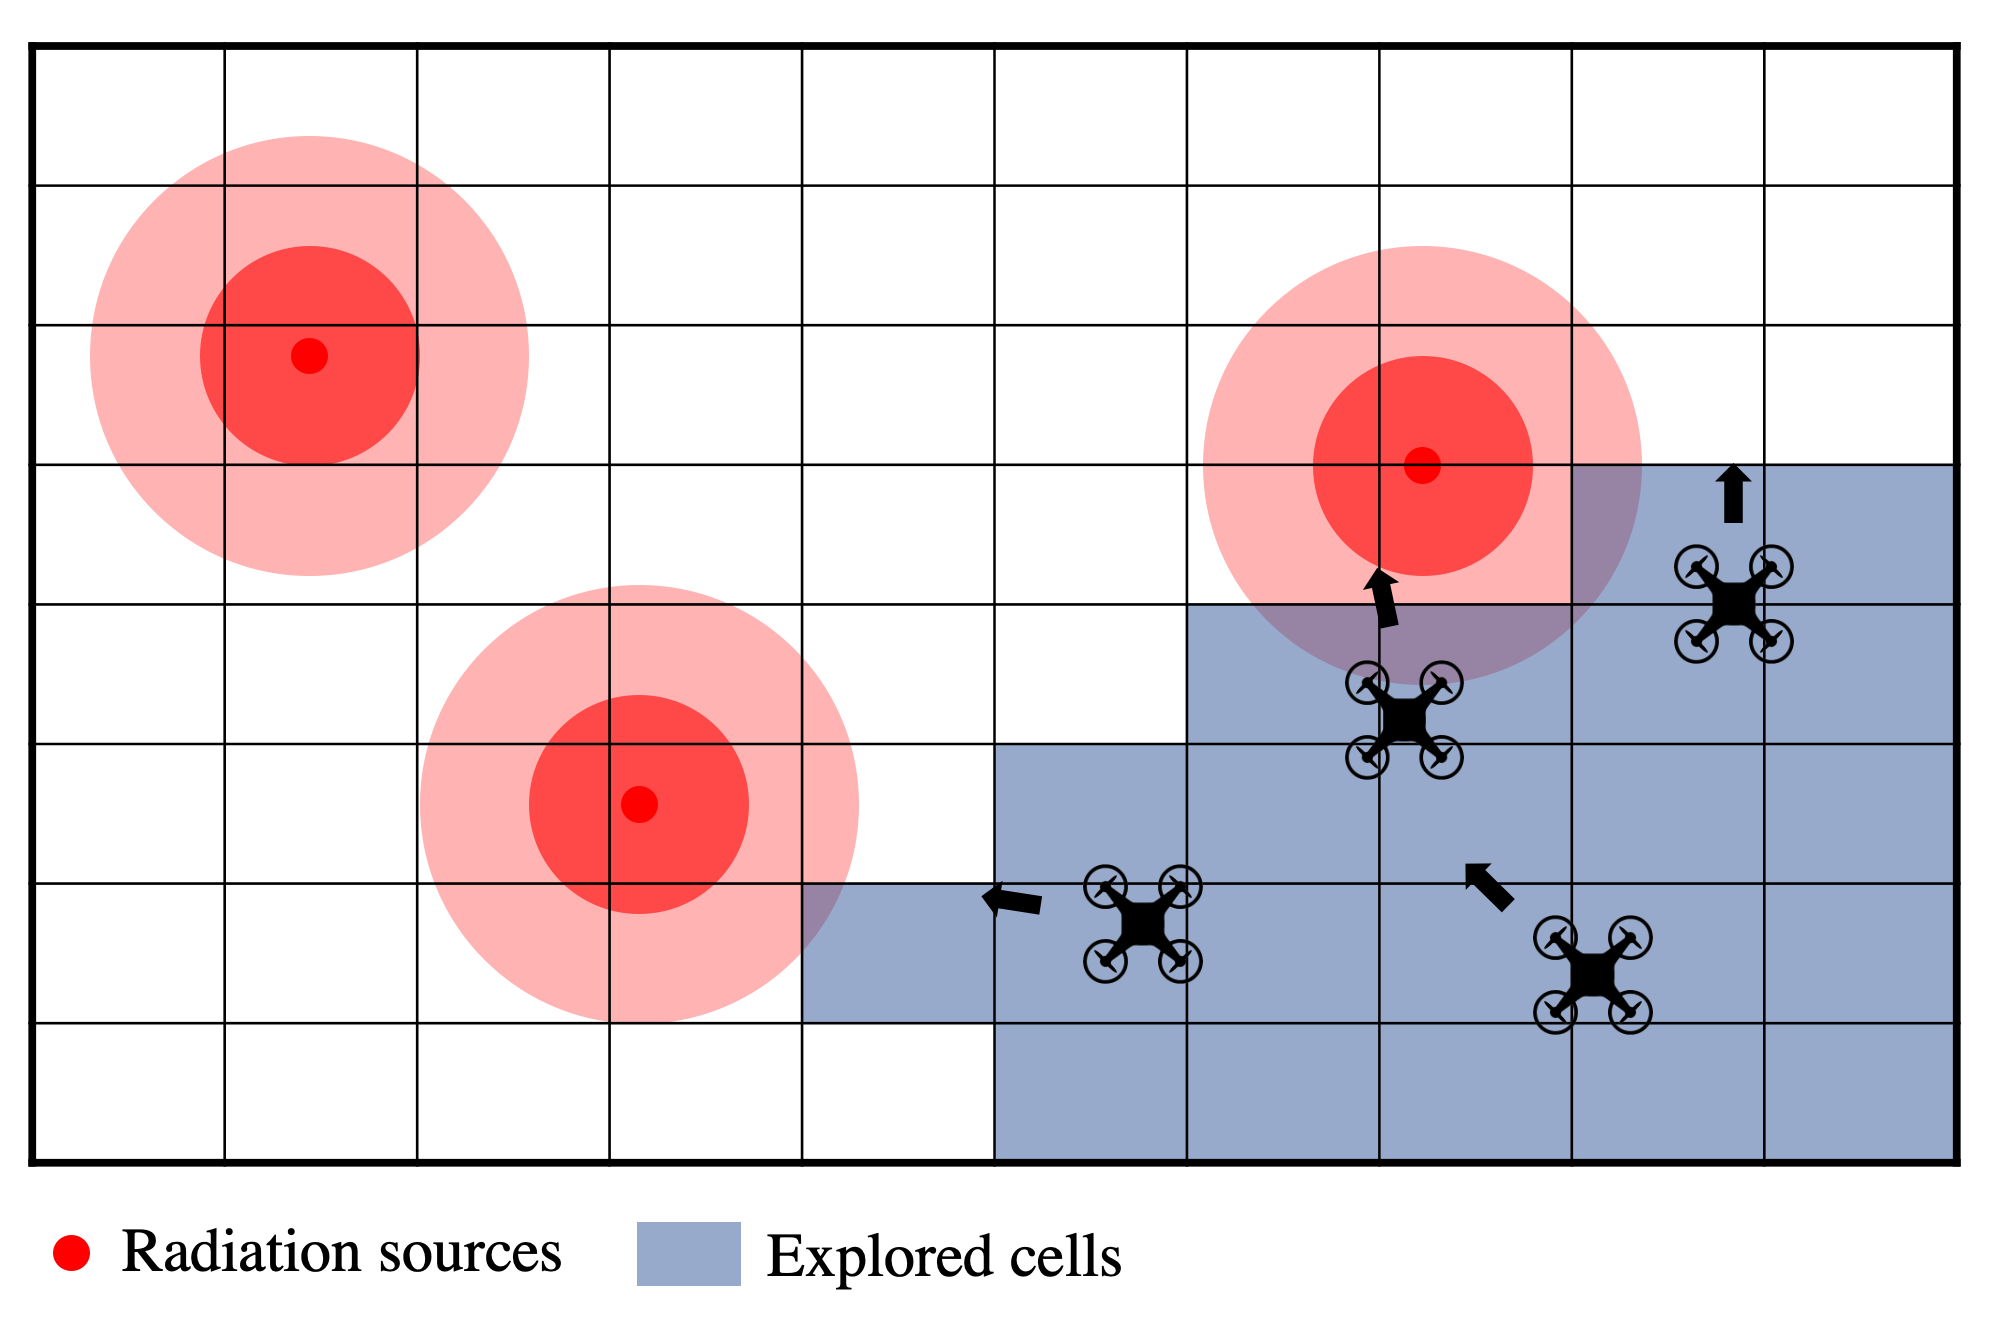
\includegraphics[width=0.70\columnwidth]{images/problemStatement1.png}
    \caption{Exploration of an unknown environment with a team of robots}
    \label{statementDORA1}
\end{figure}

\begin{figure}[H]
	\centering
    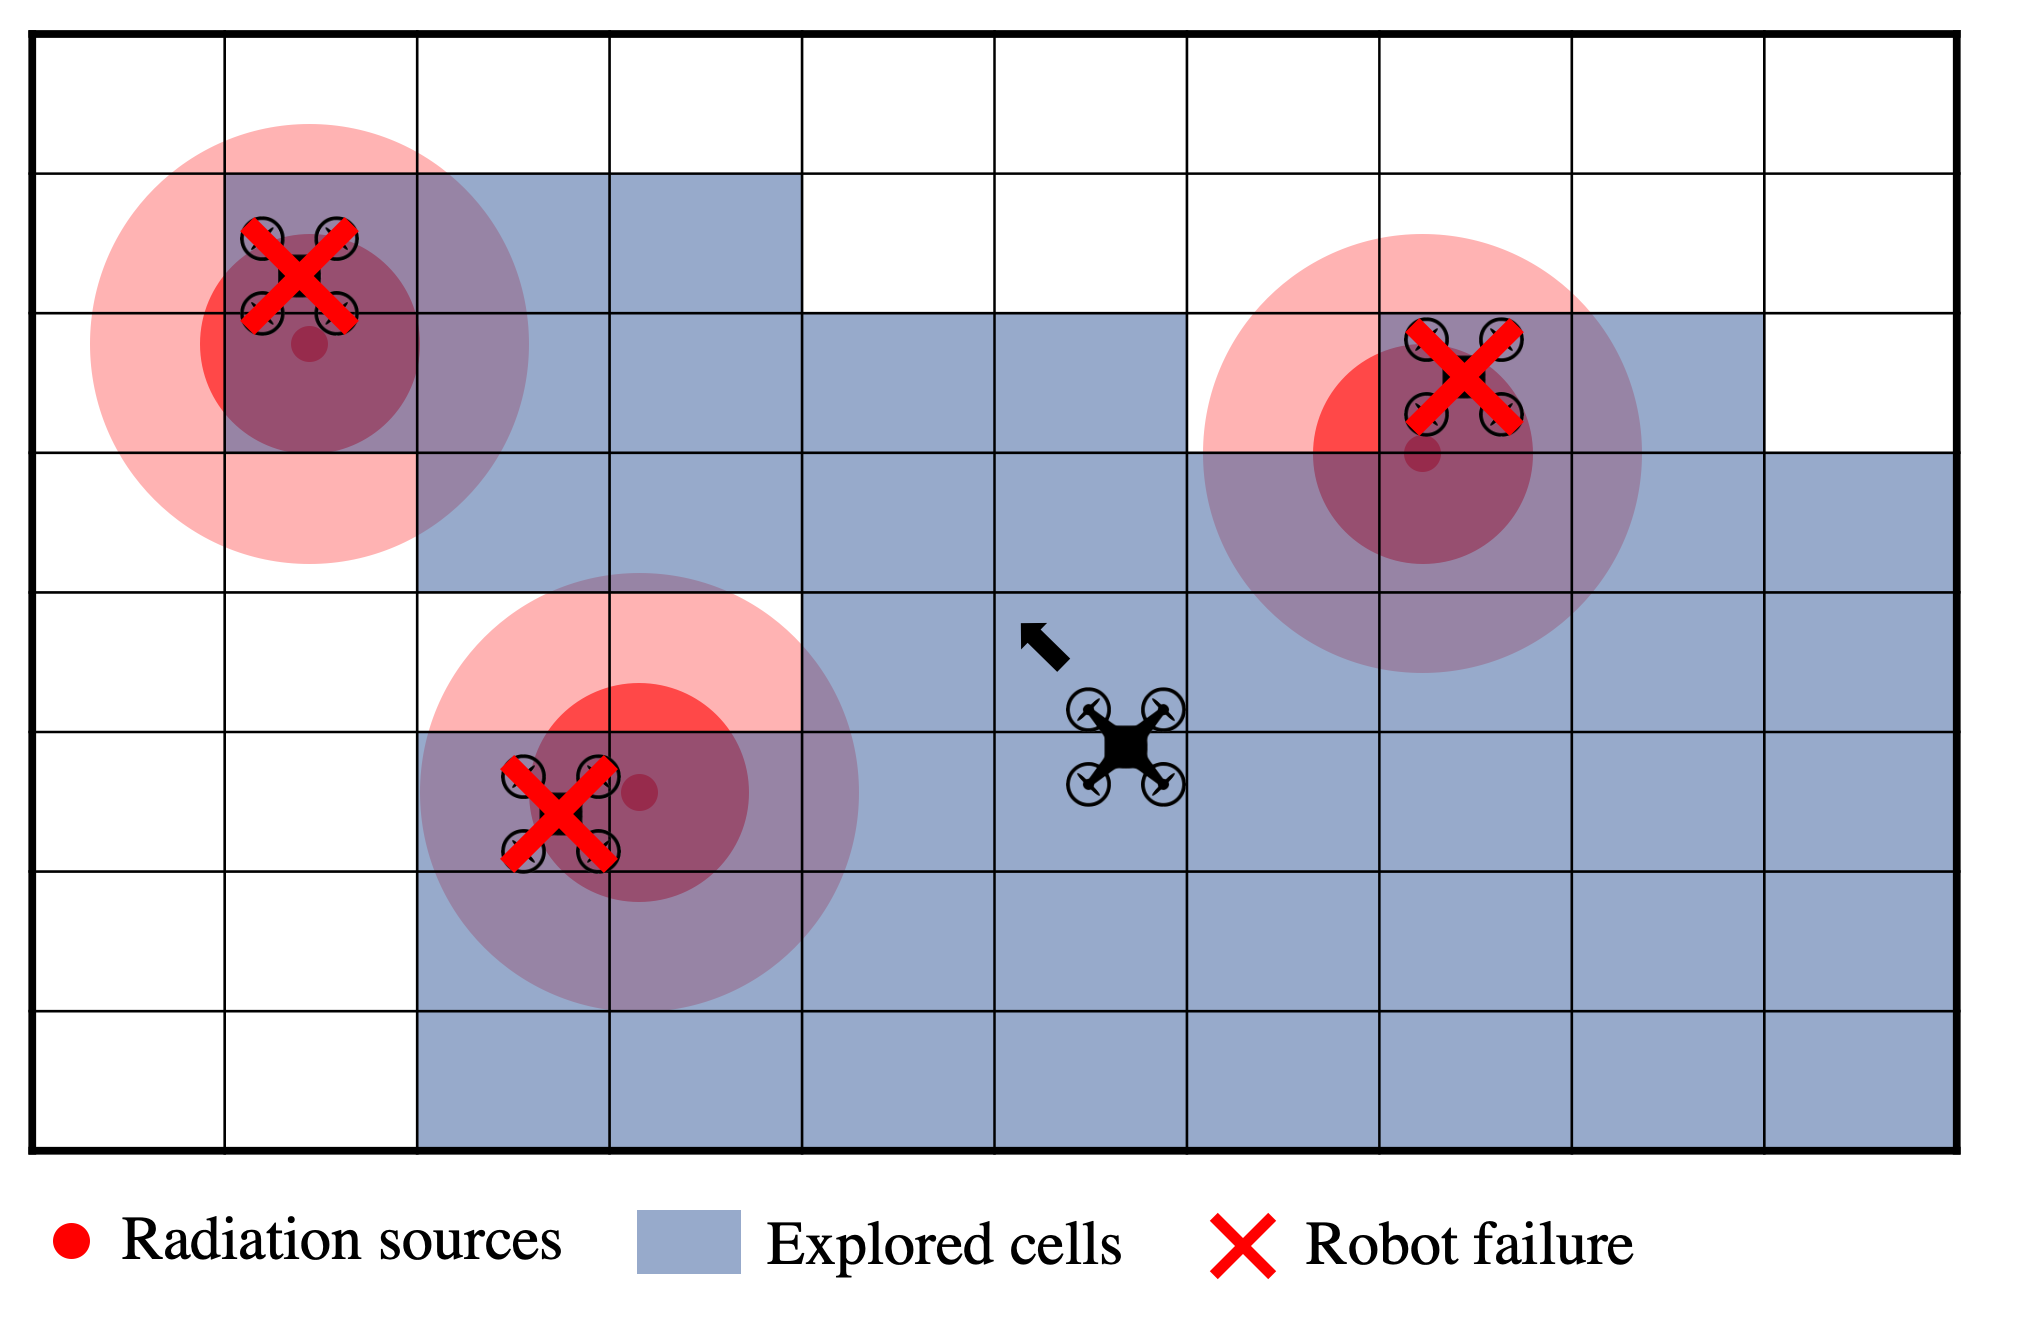
\includegraphics[width=0.70\columnwidth]{images/problemStatement2.png}
    \caption{Exploration of an unknown environment with a team of robots affected by failures.}
    \label{statementDORA2}
\end{figure}


\subsection{Information Gathering}
\label{sec:problemInformation}
Naturally, a similar problem statement can be expressed in terms of information gathering. Again, carrying the mission with numerous robots should result in a faster information gathering. However, if robots collecting information are susceptible to data corruptions, not taking risk into account will lead to inferior data collection performances. This is especially true for robot swarms operating in poorly connected environments, where directly sending the acquired data items to permanent external storage is not always possible. The robots often need to store the information locally and the robotic system acts as a temporary storage infrastructure. Assuming that environmental hazards might compromise some of the robots of the system, determining which ones are the best-suited for storing information becomes essential for reducing the likelihood of data losses. This intuition is presented in Figure \ref{statementRASS}. In figure \ref{statementRASS}, robots are dispatched in an unknown environment with the task of gathering information about it. Because the environment contains dangers, in our case a point radiation source, data items collected by robots may become corrupted if exposed to it. Transiting collected data items through robots located near a radiation source will therefore increase the likelihood of corruption. In figure \ref{statementRASS}, the lower route, although more direct towards the base station, is definitely more dangerous than the upper one. To reduce the likelihood of data losses, robots could use the upper route to reach the base station. This is the problem statement of RASS, the second algorithm of the thesis. RASS solves the problem by avoiding risky nodes of the system in its storage and routing scheme.

\begin{figure}[h]
	\centering
    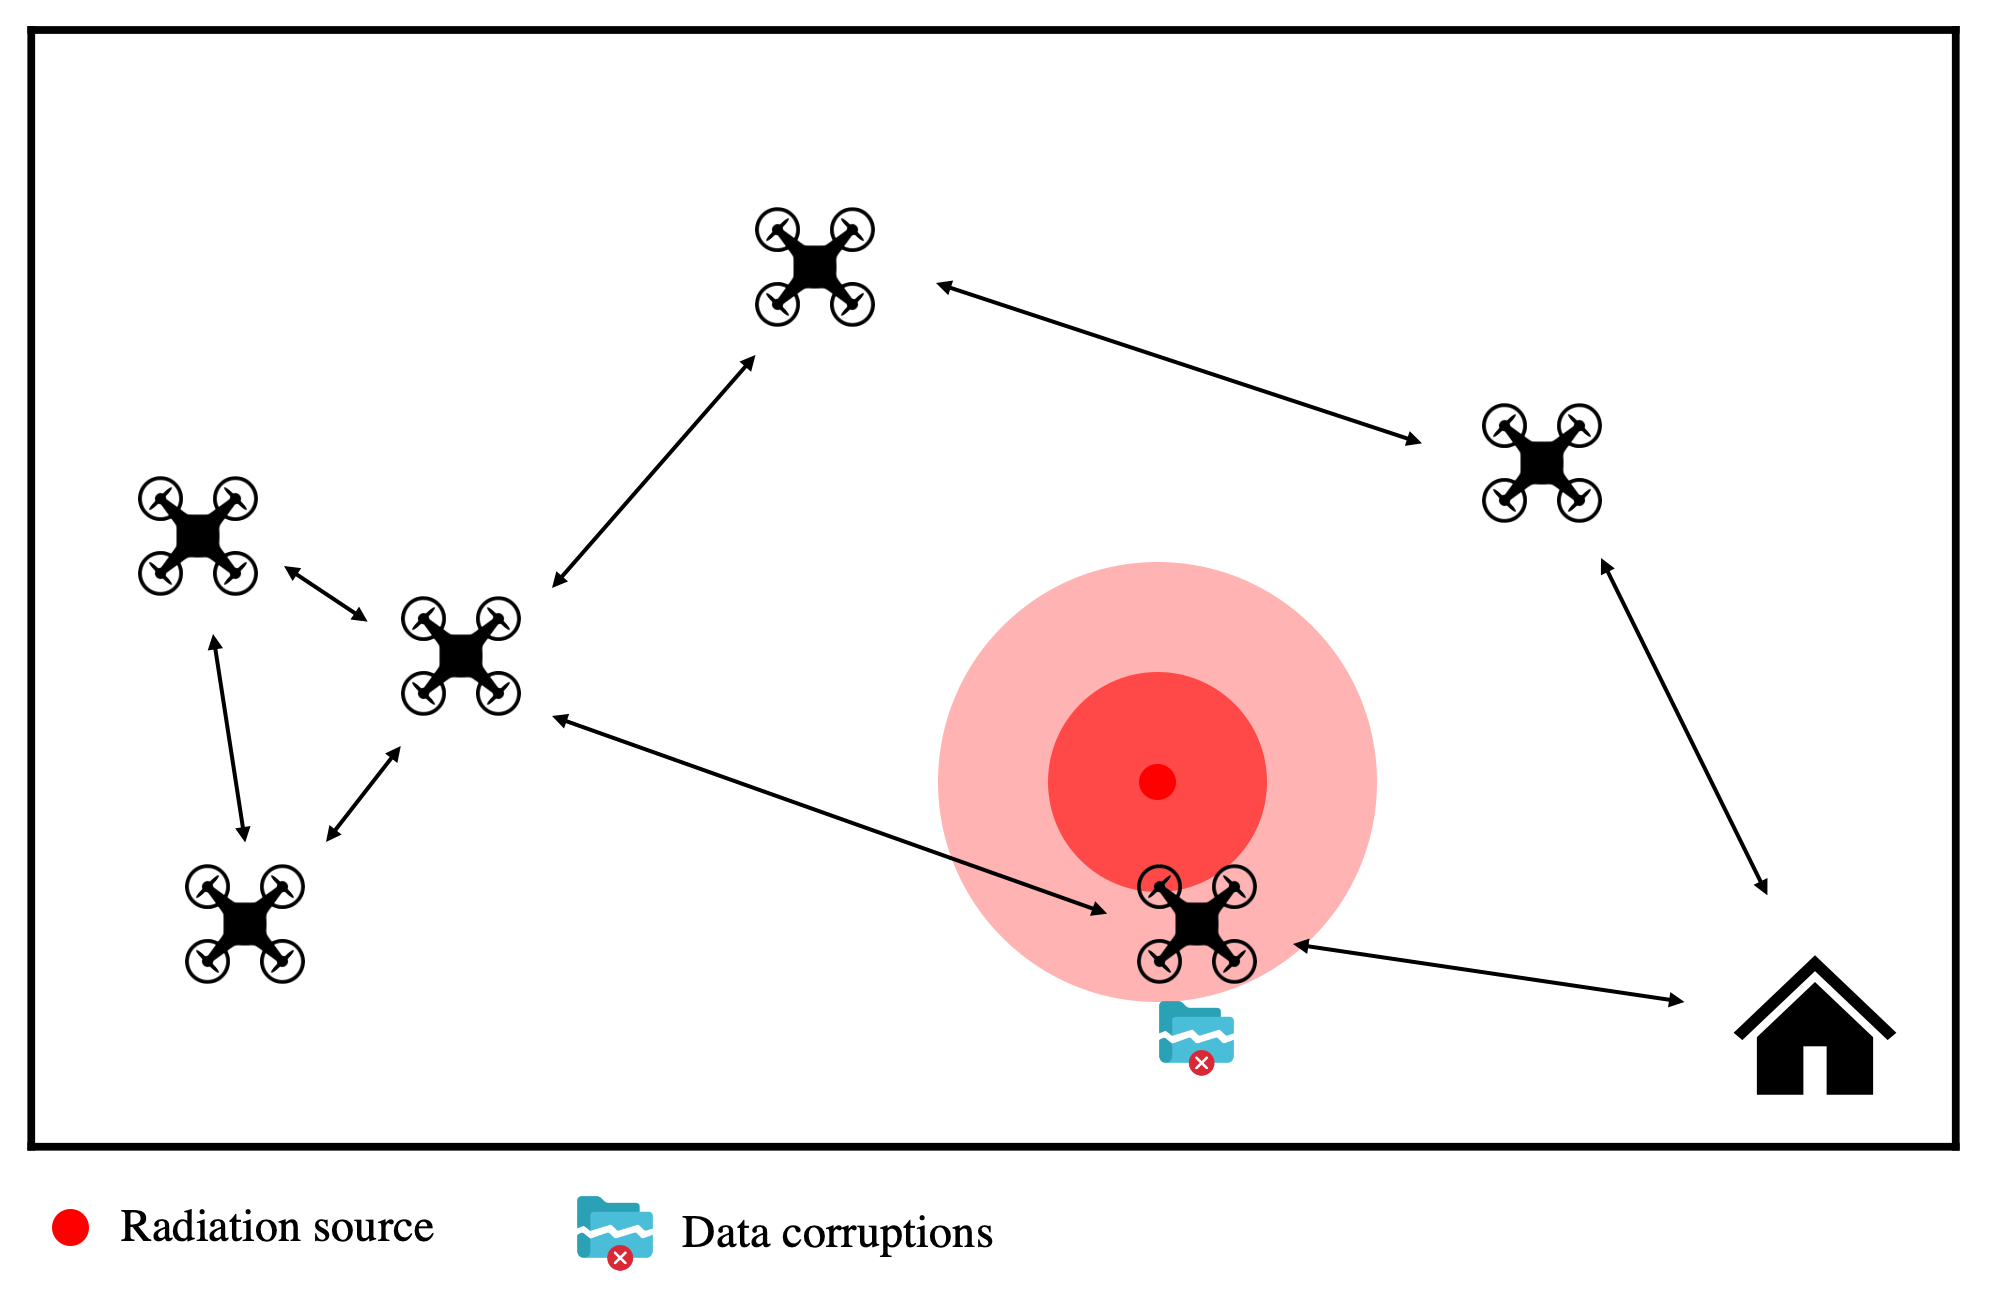
\includegraphics[width=1\columnwidth]{images/statementRASS.png}
    \caption{Information gathering in an hazardous environment}
    \label{statementRASS}
\end{figure}


\section{Research Objectives} 
\label{sec:objectifs}

Developing robot swarm algorithms to perform exploration missions in potentially dangerous environments has been the primary research objective of this master's degree. As mentioned in the previous section, this is of great importance as failures resulting from excessive exposure to risk will inevitably reduce the performance of the swarm. 

\subsection{Risk-aware Coverage}
In this regard, we first focus on bringing risk awareness to a terrain coverage algorithm, something that was lacking in the literature. Explicitly, the developed coverage algorithm should reduce considerably the failure rate of the robots carrying the exploration mission when compared to other state-of-the-art algorithms. Of course, the proposed solution should also achieve comparable terrain coverage performances when compared to these same state-of-the-art algorithms. Because the developed algorithm is intended for robot swarms, it also needs to respect the swarm robotics design principles seen in the previous section. With these objectives in mind, the algorithm should address the problem elements specific to terrain coverage in dangerous environments from section \ref{sec:problemCoverage}. To summarize, the research objectives related to terrain coverage in dangerous environments are listed below:

\begin{enumerate}
    \item Reduce failure rate compared to other state-of-the-art algorithms;
    \item Achieve comparable terrain coverage compared to other state-of-the-art algorithms;
    \item Respect swarm robotics design principles;
    \item Test real-world applicability with experiments on physical robots;
\end{enumerate}


\subsection{Risk-aware Information Gathering}
Second, we focus on risk awareness to the specific problem of information gathering performed in potentially dangerous environments, as seen in section \ref{sec:problemInformation}. The related research objectives are the following: The proposed solution should reduce notably the rate of data items that are lost due to the environmental dangers. Also, the developed solution should provide adequate transfer speeds, defined as the time it takes for data items to reach the base station after creation. Again, it will need to respect the swarm robotics design principles as it is intended to be deploy on robot swarms. To summarize, the research objectives related to information gathering in dangerous environments are listed below:

\begin{enumerate}
    \item Reduce data corruption rate compared to other state-of-the-art algorithms;
    \item Achieve comparable transfer speed compared to other state-of-the-art algorithms;
    \item Respect swarm robotics design principles;
    \item Test real-world applicability with experiments on physical robots;
\end{enumerate}


\section{Thesis outline}
The remainder of the thesis is structured as follows. In chapter \ref{sec:RevLitt}, a literature review of relevant related works is presented. The following topics will be studied in the literature review: swarm robotics, swarm programming, information sharing, routing mechanisms, swarm exploration strategies, risk in swarm robotics and some notable fault detection methods. Following the literature review, in chapter \ref{sec:approach}, the scientific approach used to meet the research objectives will be presented. Then, in chapter \ref{sec:Theme1} the algorithm DORA-Explorer, which uses risk awareness in its exploration strategy, will be presented. Subsequently, chapter \ref{sec:Theme2} will cover RASS, a risk-aware storing and routing mechanism designed for robot swarms carrying exploration missions. A high-level discussion on the results obtained throughout the master's degree in relation with the research objectives will follow in chapter \ref{sec:discussion}. Finally, in chapter \ref{sec:Conclusion}, a conclusion is presented alongside the limitations of the work and interesting future research directions.
       % Introduction au sujet de recherche.
\Chapter{LITERATURE REVIEW}\label{sec:RevLitt}
The following chapter is an overview of the existing works found in the literature in relation with the research fields covered in the thesis. Attention will be brought to swarm programming languages and tools, information sharing in robot swarms, routing mechanisms, swarm exploration strategies, risk in swarm robotics and finally fault detection methods. 

\section{Swarm programming}
Drona \cite{desai2017drona} is a state-machine-based language providing decentralized motion planning for mobile drones. It can be run on the \ac{ROS} \cite{quigley2009ros} and offers real-time collision-free planning even with not perfectly synchronized clocks between robots. This is particularly useful as perfect clock synchronization is hard to achieve, especially in large and dynamic networks \cite{cao2021distributed}. However, Drona does not consider heterogeneous robot swarms.

Koord \cite{ghosh2020koord}, a new programming language for distributed robotic applications draws considerable attention to verification and validation of the distributed algorithm. Koord provides abstraction from the physical robot and enables easy verification of the code. Its modularity and hardware-independence means that each part of the algorithm can be easily tested and validated.

A programming language, specifically designed for large-scale robot swarms, has been proposed in \cite{pinciroliBuzz2016}. Buzz is an extensible programming language for heterogeneous robot swarms offering means of easily defining swarm behaviours both from a bottom-up and top-down perspective. Of course, Buzz respects the design principles of swarm robotic systems and self-organization is assured by the fully distributed run-time platform of the language. In addition to being an accessible swarm robotics programming tool, Buzz contains a large variety of the most common swarm behaviors, such as flocking, shape formation or barriers. It therefore enables fast prototyping and reduces the need for reprogramming these common swarm behaviors. The swarm-oriented programming language has also been integrated to \ac{ROS} \cite{st2017ros}.

ARGoS \cite{Pinciroli:SI2012} is a physics-based multi-robot simulator designed for large-scale experiments of heterogeneous swarms. ARGoS is time efficient thanks to its capability of running robots on separate threads. Experimental results demonstrate that simulation run-time increases linearly with the number of robots. The simulator is highly customizable where the simulated environment can be divided into subspaces with different physics engines. Moreover, Buzz and ARGoS can work together particularly well. Swarm behaviors implemented using the Buzz programming language can be easily tested in the ARGoS simulator, even with large robot swarms. Because of the physics incorporated in the simulator, the behaviors displayed in the ARGoS usually translate well to real-world scenarios. The combination of Buzz and ARGoS provides an accessible and fast swarm robotics development tool. 

\section{Information sharing}
Distributed sensing and information sharing is not trivial, especially considering the challenges of consistency and partial connectivity among the
robotic team~\cite{amigoni2017multirobot,otte2018emergent}. In social insects, pheromone trails are used to build a shared memory structure in the environment. For example, ants that communicate between each other by laying pheromones on the ground to guide peers towards food \cite{bonabeau1999swarm}. Such distributed memory mechanism is called stigmergy \cite{heylighen2016stigmergy1, heylighen2016stigmergy2} and allows agents to interact with each other without the need for direct communication and centralized control. 

The virtual stigmergy presented in \cite{pinciroliTuple2016} and implemented in the Buzz
programming language \cite{pinciroliBuzz2016} achieves consensus among
a group of robots using Conflict-free Replicated Data Types (CRDTs),
represented as key-value pairs shared and replicated among the swarm members. This sort of shared data structure is particularly relevant for belief maps, since it is easy to assign a unique key to each cell based on its location.  In the virtual stigmergy, data is shared on writing and reading the CRDT, with the
additional updates on read improving the robustness to temporary
disconnections and message drops. This solution differs from
distributed hash tables, which require a complete view of the system
at every point in time. Essentially, information updates are propagated throughout the swarm using the stigmergy whenever it is possible. In this sense, it offers high availability while settling for eventual data consistency. However, since the information is fully replicated among the agents of the system, storing large data items can prove challenging. SOUL \cite{varadharajan2020soul}, a file sharing protocol addresses the problem by storing information in the form of (key, blob) pairs. The blob’s metadata is fully replicated across the swarm, but the blobs are decomposed into datagrams stored on specific nodes of the system. Other distributed data storage approaches such as SwarmMesh \cite{majcherczykSwarmmesh2020} store data in different
locations based on a fitness function instead of replicating them on
all robots. This allows the storage of more data with less
communication, but robots are less likely to have access to the latest
values.

Belief maps are a simple yet powerful tool for robotic exploration.
They render a continuous surface into a discrete set of cells which is especially useful for engineering problems. It makes possible highlighting specific regions of the environment and allows the designer of the algorithm to tune the level of precision at which the environment is represented. A finer granularity will provide a more accurate representation of the environment and as a result should offer more precision. However, finer granularity usually results in higher computational costs. The cells of the belief map are used to store information about the corresponding surface they represent. They generally store a probability that indicates the confidence level to which the cell is believed to contain a specific feature. Belief maps are a generalization of occupancy maps: instead of storing only one
bit per cell to indicate the presence of an obstacle/danger, they
store obstacle/danger likelihood and offer significant improvements
for exploration \cite{stachnissMappingExplorationMobile2003}. In the
field of multi-robot exploration, early techniques leveraging belief
maps date back as far as twenty years
\cite{kobayashiSharingExploringInformation2002,kobayashiDeterminationExplorationTarget2003},
but they rely on a fixed grid size and are tested only with two
robots. More recent works also leverage belief maps for multi-robot
exploration. For example,
in~\cite{indelmanCooperativeMultirobotBelief2018}, the robots consider
both the current beliefs and the expected beliefs from future
observations to coordinate their exploration. Grid maps and belief
maps are also widely used to train deep reinforcement learning
exploration policies
\cite{hanGridWiseControlMultiAgent,panovGridPathPlanning2018}, but they often rely on a trial and error process which may select actions leading to failures \cite{garciaSafeExplorationState2012,andersenSafeReinforcementlearningIndustrial2020}.


\section{Routing}
Data storage and routing remains a challenge for robot swarms as the amount of collected data items only increases with the number of robots in the system. Because robot swarms typically suffer from bad connectivity \cite{amigoni2017multirobot}, sending collected data items directly to external storage might not always be possible. Robots often need to store locally the data items until a path towards permanent storage becomes available. Because robots usually have limited communication range, the data items collected during the mission may need to be routed through multiple robots before reaching the external storage infrastructure. The multi-robot system becomes a temporary storage infrastructure and deciding where to store and send the data items become essential.
One of the most popular approaches for routing data items in swarm robotics is to use a gradient-based routing scheme \cite{faruque2005analysis,draves2004comparison,watteyne2009implementation}. In gradient-based routing, a scalar value (also called height) is assigned to each of the nodes of the system. The value is based on a metric that evaluates how fit this node is to be used in the routing scheme. For example, in a simple hop count based routing protocol, the scalar value would increase with the distance with the base station. Then, the nodes through which data items are routed are simply chosen by using the neighbor that displays the lowest height. Probably the most used metric for defining the height of the nodes is hop count \cite{kuruvila2005hop,zhang2014efficient,al2019efficient} as it allows fast and efficient routing of data items. However, other cost functions for determining the height of the nodes are possible.

Recently, many routing strategies have been developed for vehicular ad hoc networks (VANETs). In \cite{tripp2019survey}, a survey on routing protocols for such networks is presented. The survey focuses on routing protocols that use several metrics as they have shown to be effective in dynamic networks. Specifically, protocols based on the nodes' geographic positions are the most adequate as the dynamicity of the network is directly included in the routing scheme \cite{boussoufa2018geographic, fussler2002comparison}.

Other notable routing mechanisms take inspiration from nature. In \cite{li2011slime,jiang2018toward}, path growth routing protocols based on slime molds are presented. In \cite{jiang2018effective,liao2008data}, ant colony optimization-based routing algorithms are presented. The ant colony optimization algorithm tries to reproduce the behavior of ants in their search of the nearest food sources \cite{dorigo1996ant}. In the process, ants lay pheromones on the ground. Hence, the shorter the path between the nest and the food source, the more frequent it will be traversed by ants, thus increasing the pheromone intensity. Ants then follow paths with high pheromone intensities. In \cite{liao2008data} existing approaches are investigated and a hybrid routing mechanism that combines ant colony optimization and hop count into one routing scheme is proposed. However, these approaches are tailored for static topologies and are ill suited for dynamic robotic networks.


\section{Swarm exploration strategies}
Many distributed exploration strategies maximizing the amount of
terrain coverage have been proposed. The first approaches to stand out
in this regard are Voronoi-based coverage control
techniques~\cite{arslan2016voronoi,luo2019voronoi}.
Specific to \cite{luo2019voronoi}, connectivity awareness is included in the Voronoi-based coverage to guarantee that a minimum of connectivity is maintained between the robots of the system. 

A second method covers time-varying domains, in which points in the
covered region can become more or less interesting to explore,
therefore prompting a change in the coverage function
\cite{santos2019decentralized,xu2019multi}. 

Another method to optimize coverage is Frontier-Based Exploration (FBE)
\cite{yamauchi1998frontier} of which many variations have been
developed, such as those based on Particle Swarm Optimization
\cite{wang2011frontier} or the Wavefront Frontier Detector
\cite{topiwala2018frontier}. FBE's key principle is to assign one of three states to the cells constituting the environment:

\begin{itemize}
\item \textbf{Explored:} cells that have already been explored
\item \textbf{Frontier:} cells between explored and unexplored space
\item \textbf{Unexplored:} cells that remain uncovered
\end{itemize}

Using the state of the cells, robots coordinate to explore the regions at the frontier, thereby expanding them and eventually achieving full map coverage.

Other interesting coverage techniques take inspiration from insects and leverage virtual pheromones for encouraging or discouraging robots to explore specific regions of the environment. For example, in ant foraging, negative feedback in the form of pheromones is used to discourage ants from using unprofitable paths \cite{robinson2005no}. In \cite{hunt2019testing}, pheromones are employed to dissuade robots of covering already covered areas of the environment. Authors show that using repellent pheromones can effectively encourage a rapid dispersal of robots even in large swarm systems. In Phormica \cite{salman2020phormica}, robots start exploring the environment in a random fashion. By projecting \ac{UV} light on the ground, the robots are able to convey information to their peers and let them know that the region has already been covered. When the artificial pheromone is detected, robots can change their course of action and move towards unaltered regions of the environment.

However, none of these aforementioned coverage strategies take
risk into account. In
\cite{dames2012decentralized,schwagerMultirobotControlPolicy2017}
an exploration algorithm that maximizes information gain in the presence of unknown hazards is presented. Unfortunately, this optimal algorithm has a
very high computational complexity and could benefit from approximations.



\section{Risk in swarm robotics}
The importance of risk management has dramatically increased over the last few years. Robotic systems are being used more widely and as a result, risk management becomes essential as to not endanger the system itself and the objects and beings in its immediate environment. The importance of enabling distributed situational awareness in robot swarms is raised in \cite{jones2020distributed}. In \cite{hunt2020checklist}, a checklist for robot swarms to be safe for the public, the environment and for itself is presented. The authors draw attention to the lack of proper systematic swarm safety assessment mechanism and propose a checklist, in the form of ten questions, that should be answered when designing such systems. They consider that swarm safety is larger than simply analyzing failure modes. Questions related to ethics, legality, accountability, security are also listed and as a result, should provide a more thorough consideration of all socio-technical risks robot swarms face. 

In \cite{higgins2009threats}, the security challenges of robots swarms are presented. Security is defined as the state of being protected from risks originating from hostile and malicious intentions. The security of new technologies is usually not included in its design process, typically it is with the rise of the technology that security concerns appear. To prevent any unwanted consequences, the paper presents the security challenges robot swarms will face in an attempt of including this component in the design process of the new technology. However, only security threats are considered and risk, as something not malicious, is not examined.

Several path planners based on Markov Decision Processes \cite{undurti2010online,thiebaux2016rao,xiao2020robot} take into account risk and have useful definitions of it. In \cite{xiao2020robot}, risk is categorized into three different groups:

\begin{itemize}
    \item \textbf{Locale-Dependent:} Risk elements not depending on history. The risks associated with this category are usually location-based, in other words, it is the position of the robot in the environment that determines the level of risk. 
    \item \textbf{Action-Dependent:} Risk elements depending on close history, specifically changes of states. For example, the risk associated with an aggressive turn is tied to the last states of the robot.   
    \item \textbf{Traverse-Dependent:} Risk elements depending on the entire history of the robot. Risks associated with this category are tied to all the states traversed by the robot. For example, risk associated with low battery levels are included in the category.  
\end{itemize}

In \cite{hakobyan2019risk}, a risk-aware motion planning and decision-making mechanism is presented. They automatically adjust the "conservativeness" of the motion-planner based on the risk a robot faces. The paper uses a conditional value-at-risk method used in finance to estimate the risk of an investment. They use a safety risk measure from \cite{samuelson2018safety} onto which they apply the conditional value-at-risk method to achieve safe motion planning and control. Unfortunately, risk only includes collisions and does not translate to other types of hazard robots could face. Value-at-risk strategies for robot swarms in hazardous environments were also studied in \cite{hunt2021value}. Again, the method of value-at-risk allows quantifying the foreseen loses over a period of time where the environment contains potentially damaging radiation sources. In detail, agents of the swarm calculate the value-at-risk at every time step and share it with their neighbors when their value-at-risk limit is exceeded. The information helps team members avoid dangerous locations of the environment and overall decreases exposure to risk. Some shortcomings of the method include the determination of the value-at-risk limit and the lack of instantaneous responsiveness of the method as it relies on past observations. Overall, the value-at-risk methods show that financial risk management techniques are an interesting avenue for risk awareness in swarm robotics.

Another interesting idea for risk awareness is proposed in \cite{ono2008efficient,vitus2011feedback}, where a "risk budget" is allocated to their agents, allowing them to optimize a balance between risk and reward to guide robots. However, these systems assume knowledge of the global state of the environment, which is unavailable when exploring unknown environments. Furthermore, most are only applied to single-robot systems. 

In SPIDER \cite{hunt2020spider}, multiple agents are tasked with chain formation in dangerous environments. They adapt to varying levels of risk to be resilient to significant failures and member losses in order to maximize information gathering. They introduce a level of "boldness" which represent the risk appetite of the agents of the swarm. This risk appetite is modulated by the connectivity of the agent, specifically its frequency of interactions of neighbors. When an agent is well connected, its risk appetite grows and, as a result, should be encouraged to explore new parts of the environment. On the other hand, an agent that is isolated and far from any other members of the swarm will increasingly display a shy behavior and go back to safer areas of the environment. SPIDER effectively allows a swarm to trade off the benefits of information gain versus robot failures. However, the problem is only studied for a chain formation scenario and risk is only a measure of how well connected is an agent.  






\section{Fault detection}

A taxonomy of the faults affecting robotic systems is presented in \cite{khalastchi2018fault}. Hardware faults affect physical components of the system. They compromise the sensing and acting abilities of the robots. Software faults affect the behaviour of the robots and are caused by faulty algorithms and/or faulty implementations. Interaction faults affect the dynamics of the robotic system and are caused by exogenous events. Hopefully, fault detection methods have been developed to mitigate the presence of faults in robotic systems. They are divided into three big families: data-driven; model-based; knowledge-based \cite{khalastchi2018fault}. 

\begin{itemize}
\item \textbf{Data-driven} approaches use sensor data and compare it to known faults, to past normal/abnormal behaviors or to the behavior of neighbour agents. Using statistical tools, data-driven approaches compute the deviation of the data and classify it as normal/abnormal depending on the extent of this deviation.
\item \textbf{Model-based} approaches use an \textit{a priori} explicit model of the system to identify faults. The model is a set of analytical equations or logical formulas. When an irregularity is identified between what is observed and the theoretical model, a fault is presumed. The main drawback of these approaches is the work needed in constructing the theoretical model. 
\item \textbf{Knowledge-based} approaches are similar to the way a human would perform fault detection. A fault is quickly associated with its cause. Faults are typically represented in a tree structure where the fault can be linked backwards to where it originated. It is particularly useful for fault isolation.
\end{itemize}

Outlier detection methodologies have been widely used for identifying anomalies that could be the result of a fault. A definition of “outlier” was proposed by Grubbs (Grubbs, 1969): 

\begin{center}
\textit{An outlying observation, or outlier, is one that appears to deviate
markedly from other members of the sample in which it occurs.}
\end{center} 

Outlier detection is used for classifying data as normal or abnormal. Applying it to fault detection is to suppose that the abnormality observed is the result of a fault. Outlier detection is part of the data-driven family of the fault detection approaches. From \cite{hodge2004survey}, outlier detection can be divided into 3 types: 

\begin{itemize}
    \item \textbf{Unsupervised clustering:} The outlier detection does not need any prior knowledge of the data. Using the distribution of the data, the most isolated points are classified as outliers.
    \item \textbf{Supervised classification:} The outlier detection needs a prior knowledge of normality and abnormality. Using pre-labelled normal/abnormal data, new incoming data can be classified in either of these classes based on its distance. 
    \item \textbf{Semi-supervised recognition:} The outlier detection needs prior knowledge of normality. Using pre-labelled normal data, new incoming data can be classified as normal or abnormal. It resembles type 2 outlier detection but without the need for labelled abnormal data.
\end{itemize}


Additionally, two strategies can be used for fault detection: endogenous fault detection and exogenous fault detection \cite{christensen2008fault, lau2012error, Miller2021modern}. Endogenous fault detection refers to the actions taken by an individual to perform fault detection on itself and on its own. While this approach is well suited for single robots, in the context of multi-robot systems, opting for this approach does not take advantage of the multiple entities close to one another forming the swarm. On the other hand, exogenous fault detection refers to the actions taken by neighbour robots on a central entity. This approach relies on the observations of multiple robots and is, as a result, better suited for swarm robotics. Exogenous data-driven fault detection methods are the best suited for robot swarms. Exogenous strategies leverage the power of swarms through collaboration of all team members. Data-driven methods allows the detection of previously unseen faults and, as a result, enable the deployment of the swarm in unknown and dynamic environments.


A fault detection method inspired by the human immune system has been proposed in \cite{ tarapore2015err, tarapore2017generic}. The method uses the mathematical formulation of the cross-regulation model to distinguish between normal and abnormal behaviors in a swarm of robots. Abnormality is the indication of a fault, the abnormality being the result of it. The fault detection method is divided into three main phases: (i) observing the behaviors of the agents; (ii) based on the observed behaviors, perform anomaly detection using the cross-regulation model; (iii) voting to decide if the agent’s behavior is normal or abnormal. The first phase of the method (i) uses feature vectors to characterize the behavior of an agent. The feature vector contains six features $(F_1, F_2, F_3, F_4, F_5, F_6)$, each indicating the presence $(Fi=1)$ or absence $(Fi=0)$ of a particular behavior. Then, the method uses these informative binary feature vectors for running the cross-regulation model (ii). In this fault detection method, if at the end of the cross-regulation cycle, the \ac{APC} (modelled as a feature vector) is considered a foreign pathogen, an abnormality is inferred. Finally, in the last phase of the methods (iii) the agents consolidate their individual decisions and vote on the normal/faulty behavior of the neighboring agents. Agents that receive more than five “foreign pathogen” votes are considered faulty. The method was tested on a swarm of seven physical robots and results showed that the method was able to reliably identify the faults injected in the system \cite{tarapore2019fault}. The efficiency of the method actually surpassed the ones of other traditional outlier detection methods, namely \ac{KNN} and  \ac{LOF}. However, for both \ac{KNN} and \ac{LOF} binary feature vectors were used, however, these methods could benefit from using non-binary feature vectors \cite{tarapore2019fault}. The advantage of this method is that it does not require any prior knowledge of the fault to identify it. Indeed, being an outlier detection method, the presence of faults is only inferred on the presence of an abnormal behavior. This is particularly important in swarm of robots where it is very difficult to know in advance the potential fault that the system will encounter. It is also easier to implement. However, because the method identifies anomalies and not faults, it is very hard to perform diagnosis and recovery procedures. It is difficult to assess the correct plan of action when the nature of the problem remains unknown. In \cite{okeefe2018adaptive}, the problem is solved by introducing a fault diagnosis layer after the fault detection one. 

The \ac{LOF} \cite{breunig2000lof} is a measure of how much a data point can be considered an outlier. The \ac{LOF} represents the density of a point compared to the density of its neighbors. A \ac{LOF} of around 1 means that the point is not an outlier. A \ac{LOF} much higher than 1 indicates that the density of the data point is smaller the density of the neighboring points. The data point is isolated and is, as a result, most likely to be an outlier. In summary, the higher the \ac{LOF}, the most likely the data point is an outlier. 

A neural network fault detection approach was proposed in \cite{christensen2008faultDetection}. The approach assumes that the occurrence of a fault in the robotic system will cause the flow of sensory data to change. By monitoring it and feeding it to a neural network, the method is capable of detecting faults in the system with manageable latency using s-bots robots \cite{mondada2005cooperation}. For every control cycle, sensory data is given as an input to the neural network which, in turn, outputs the state of the system (0 or 1), with 0 corresponding to not faulty and 1 to faulty. Again, this falls into the anomaly detection category and more specifically under the data-driven group. One of the drawback of the method is the need for training runs to train the neural network.

In recent years, deep learning anomaly detection methods have been developed and have shown to generally outperform the traditional anomaly detection methods \cite{pang2021deep}. They are especially effective when working with complex and large data flows where traditional methods tend to struggle.



  % Revue de littérature.
\Chapter{RESEARCH APPROACH AND THESIS ORGANIZATION}
\label{sec:approach}

This chapter will present the research approach used to meet the objectives detailed in \ref{sec:objectifs}. The link between the two works DORA-Explorer and RASS will follow and finally the document structure will be presented.

\section{Research approach}
Bringing risk-awareness and increasing robustness of swarm algorithms has been the primary focus of the master's work. Because the laboratory into which the master's degree was carried, the Mistlab, focuses on space technologies the approach chosen to meet the identified objectives was to develop meaningful algorithms for the exploration of space. In this regard, an exploration algorithm DORA-Explorer was built and enables efficient exploration of an unknown environment while avoiding its hazardous locations. Then, with a satisfactory exploration algorithm, focus switched towards building an efficient storing and routing algorithm: RASS. This algorithm is meant to be used by robot swarm carrying the exploration task and collecting information in the process. The two algorithms are linked by their contribution to space exploration in the presence of risk. They are meant to be used side by side when exploring and gathering information about a new environment and should provide increased robustness to the swarm carrying the mission.

\section{Document structure}
The document's structure follows the one prescribed for thesis with articles. Because I am first author only for the article on DORA-Explorer, this one will be directly included in the body of the thesis under its original article format whereas the second work, RASS, will be summarized. The document is structured as follows:

\begin{itemize}
    \item Chapter 1 gives an introduction on the research subject and presents the basic concepts upon which the work done in the course of the master's degree has been built. 
    \item Chapter 2 provides relevant contributions to the master's thesis found in the literature.
    \item Chapter 3 presents the common thread between the two research project carried in the course of the master's degree
    \item Chapter 4 presents a fully decentralized and risk-aware exploration algorithm called DORA-Explorer. This work will be published in the IEEE International Conference on Robotics and Automation (ICRA) in May 2022.
    \item Chapter 5 presents a fully decentralized and risk-aware routing algorithm called RASS. This work will be published at the International Conference on Autonomous Agents and Multiagent Systems (AAMAS) as an extended abstract in May 2022. 
    \item Chapter 6 discusses about the results obtained by the two algorithms and to what extent they satisfied the objectives of the master's degree. 
    \item Chapter 7 provides a summary of the works as well as some limitations of the algorithms presented and some interesting future research directions.
\end{itemize}



 
\Chapter{DORA: Distributed Online Risk-Aware Explorer}\label{sec:Theme1}
 

\section{Abstract}
    Exploration of unknown environments is an important challenge in the
    field of robotics. While a single robot can achieve this task alone,
    evidence suggests it could be accomplished more efficiently by
    groups of robots, with advantages in terms of terrain coverage as
    well as robustness to failures. Exploration can be guided through
    belief maps, which provide probabilistic information about which
    part of the terrain is interesting to explore (either based on risk
    management or reward). This process can be centrally coordinated by
    building a collective belief map on a common server. However,
    relying on a central processing station creates a communication
    bottleneck and single point of failure for the system. In this
    paper, we present Distributed Online Risk-Aware (DORA) Explorer, an
    exploration system that leverages decentralized information sharing
    to update a common risk belief map. DORA-Explorer allows a group of
    robots to explore an unknown environment discretized as a 2D grid
    with obstacles, with high coverage while minimizing exposure to
    risk, effectively reducing robot failures.


\section{Introduction}
The exploration of unknown environments is at the core of numerous
robotic applications from search-and-rescue operations
\cite{matos2016multiple} to space
missions~\cite{fong2005interaction}. The problem has been mostly
studied in single robot setups, but the ability to perform exploration
with teams of robots opens the door to even more ambitious
applications, because with proper coordination, the time required to
explore a given environment should decrease proportionally to the
number of robots~\cite{burgard2005coordinated}. Therefore, multi-robot
exploration is an attractive solution to many time-critical
applications such as search-and-rescue operations or planetary
exploration. Moreover, multi-robot teams are usually resilient to some
amount of robot
failures~\cite{ramachandran2019resilience,wehbe2021probabilistic,winfield2006safety}. However,
robot failures are still undesirable as they can affect team
performance and should therefore be avoided, which is the main
motivation for this work, in which we present a risk-aware exploration
algorithm for multi-robot systems: Distributed Online Risk-Aware
(DORA) Explorer.

Multi-robot systems come with their own sets of constraints and
challenges: among those, coordination and communication are the most
relevant to the exploration problem. Without coordination, the robots
will inevitably explore overlapping parts of the environment, leading
to little gains in terms of efficiency compared to single-robot
solutions. While the coordination could be optimally orchestrated from
a central computing station, such a solution would require a perfect
connectivity maintenance with each robot and a high communication
bandwidth since the robots would need to send their observations and
receive their commands. This motivates the need for a decentralized
exploration algorithm relying only on local computation onboard the
robots and communication with their neighbours. To the best of our knowledge, there exists no risk-aware collaborative
exploration algorithm that relies solely on local or shared
information. Therefore, in this paper, we make the following
contribution to the field of multi-robot exploration: \textit{A
  decentralized exploration algorithm leveraging distributed belief
  maps (DBMs) to maximize coverage and decrease robot failure
  probability using risk-awareness.} To
evaluate this system, we test it on the specific problem of
\emph{hazard mapping} in a 2D world discretized as a grid, in which a
multi-robot team simultaneously explores a dangerous environment and
collaborates to avoid hazardous locations as well as obstacles. We validate our approach in a physics-based simulator, ARGoS
\cite{Pinciroli:SI2012}, in which we define a grid-based environment
with multiple radiation sources. We then test it on physical
robots and obtain convincing results. 

\section{Related Work and Background}
Distributed sensing and information sharing is not trivial, especially considering
the challenges of consistency and partial connectivity among the
robotic teams~\cite{amigoni2017multirobot,otte2018emergent}. The virtual stigmergy
presented in \cite{pinciroliTuple2016} and implemented in the Buzz
programming language \cite{pinciroliBuzz2016} achieves consensus among
a group of robots using Conflict-free Replicated Data Types (CRDTs),
represented as key-value pairs shared and replicated among the swarm members. This sort of shared data structure is
particularly relevant for belief maps, since it is easy to assign a
unique key to each cell based on its location.  In the virtual
stigmergy, data is shared on writing and reading the CRDT, with the
additional updates on read improving the robustness to temporary
disconnections and message drops. This solution differs from
distributed hash tables, which require a complete view of the system
at every point in time. Essentially, information updates are propagated throughout the swarm using the stigmergy whenever it is possible. In this sense, it offers high availability while settling for eventual data consistency. Other distributed data storage approaches such
as SwarmMesh \cite{majcherczykSwarmmesh2020} store data in different
locations based on a fitness function instead of replicating them on
all robots. This allows the storage of more data with less
communication, but robots are less likely to have access to the latest
values.

Belief maps are a simple yet powerful tool for robotic exploration
because they can represent an environment with a 2D cell grid. They
are a generalization of occupancy maps: instead of storing only one
bit per cell to indicate the presence of an obstacle/danger, they
store obstacle/danger likelihoods and offer significant improvements
for exploration \cite{stachnissMappingExplorationMobile2003}. In the
field of multi-robot exploration, early techniques leveraging belief
maps date back as far as twenty years
\cite{kobayashiSharingExploringInformation2002,kobayashiDeterminationExplorationTarget2003},
but they rely on a fixed grid size and are tested only with two
robots. More recent works also leverage belief maps for multi-robot
exploration. For example,
in~\cite{indelmanCooperativeMultirobotBelief2018}, the robots consider
both the current beliefs and the expected beliefs from future
observations to coordinate their exploration. Grid maps and belief
maps are also widely used to train deep reinforcement learning
exploration policies
\cite{hanGridWiseControlMultiAgent,panovGridPathPlanning2018}, but they often rely on a trial and error process which may select actions leading to failures \cite{garciaSafeExplorationState2012,andersenSafeReinforcementlearningIndustrial2020}.

To provide more insight into our claim that there are no risk-aware collaborative exploration strategies in  the literature, it should be noted that risk-awareness has indeed been used in some swarm systems to improve robustness. For example, several path planners based on Markov Decision Processes \cite{undurti2010online,thiebaux2016rao,xiao2020robot} take into account risk and have useful definitions of it. Another interesting idea for risk awareness is proposed in \cite{ono2008efficient,vitus2011feedback}, where a "risk budget" is allocated to their agents, allowing them to optimize a balance between risk and reward to guide robots. However, these systems assume a knowledge of the global state of the environment, which is unavailable when exploring unknown environments. Furthermore, most are only applied to single-robot systems. In SPIDER \cite{hunt2020spider}, multiple agents are tasked with chain formation in dangerous environments. They adapt to varying levels of risk to be resilient to significant failures and member losses. However, their task is significantly different from DORA Explorer's objectives.

Many distributed exploration strategies maximizing the amount of
covered terrain have been proposed. The first approaches to stand out
in this regard are Voronoi-based coverage control
techniques~\cite{luo2019voronoi,santos2019decentralized}. A second
method covers time-varying domains, in which points in the
covered region can become more or less interesting to explore,
therefore prompting a change in the coverage function
\cite{santos2019decentralized,xu2019multi}. Another method to optimize
coverage is Frontier-Based Exploration (FBE)
\cite{yamauchi1998frontier} of which many variations have been
developed, such as those based on Particle Swarm Optimization
\cite{wang2011frontier} or the Wavefront Frontier Detector
\cite{topiwala2018frontier}. However, none of these strategies take
risk into account. Therefore, the
exploration strategy implemented in this paper takes inspiration of
the multi-robot control algorithm presented in
\cite{dames2012decentralized,schwagerMultirobotControlPolicy2017}
which maximizes the information gain during exploration in the
presence of unknown hazards. However, this optimal algorithm has a
very high computational complexity and could benefit from approximations.

% We build on those approaches and address some their shortcomings by
% implementing a risk-aware exploration algorithm leveraging a DBM of
% the environment which is not constrained to a fixed size.


\section{System Model}
DORA-Explorer builds on the previously mentioned approaches and addresses some of their shortcomings, namely by leveraging risk awareness to provide better efficiency when exploring hazardous environments. Reducing the
likelihood of robot failures is of high importance as they lead to poor exploration performance. Indeed, if robots experiencing complete
failures are not replaced, individual failures lead to lower numbers
of robots carrying the exploration task resulting in a decrease of the exploration rate. We model the 2D environment as cells forming a grid
represented as $E \subset \mathbb{Z}^2$. The team of robots is denoted
as the collection of agents $a_i \in A$.

% \begin{figure*}[h]
%     \centering
%     % \begin{subfigure}{0.40\textwidth}
%     %      \centering
%     %      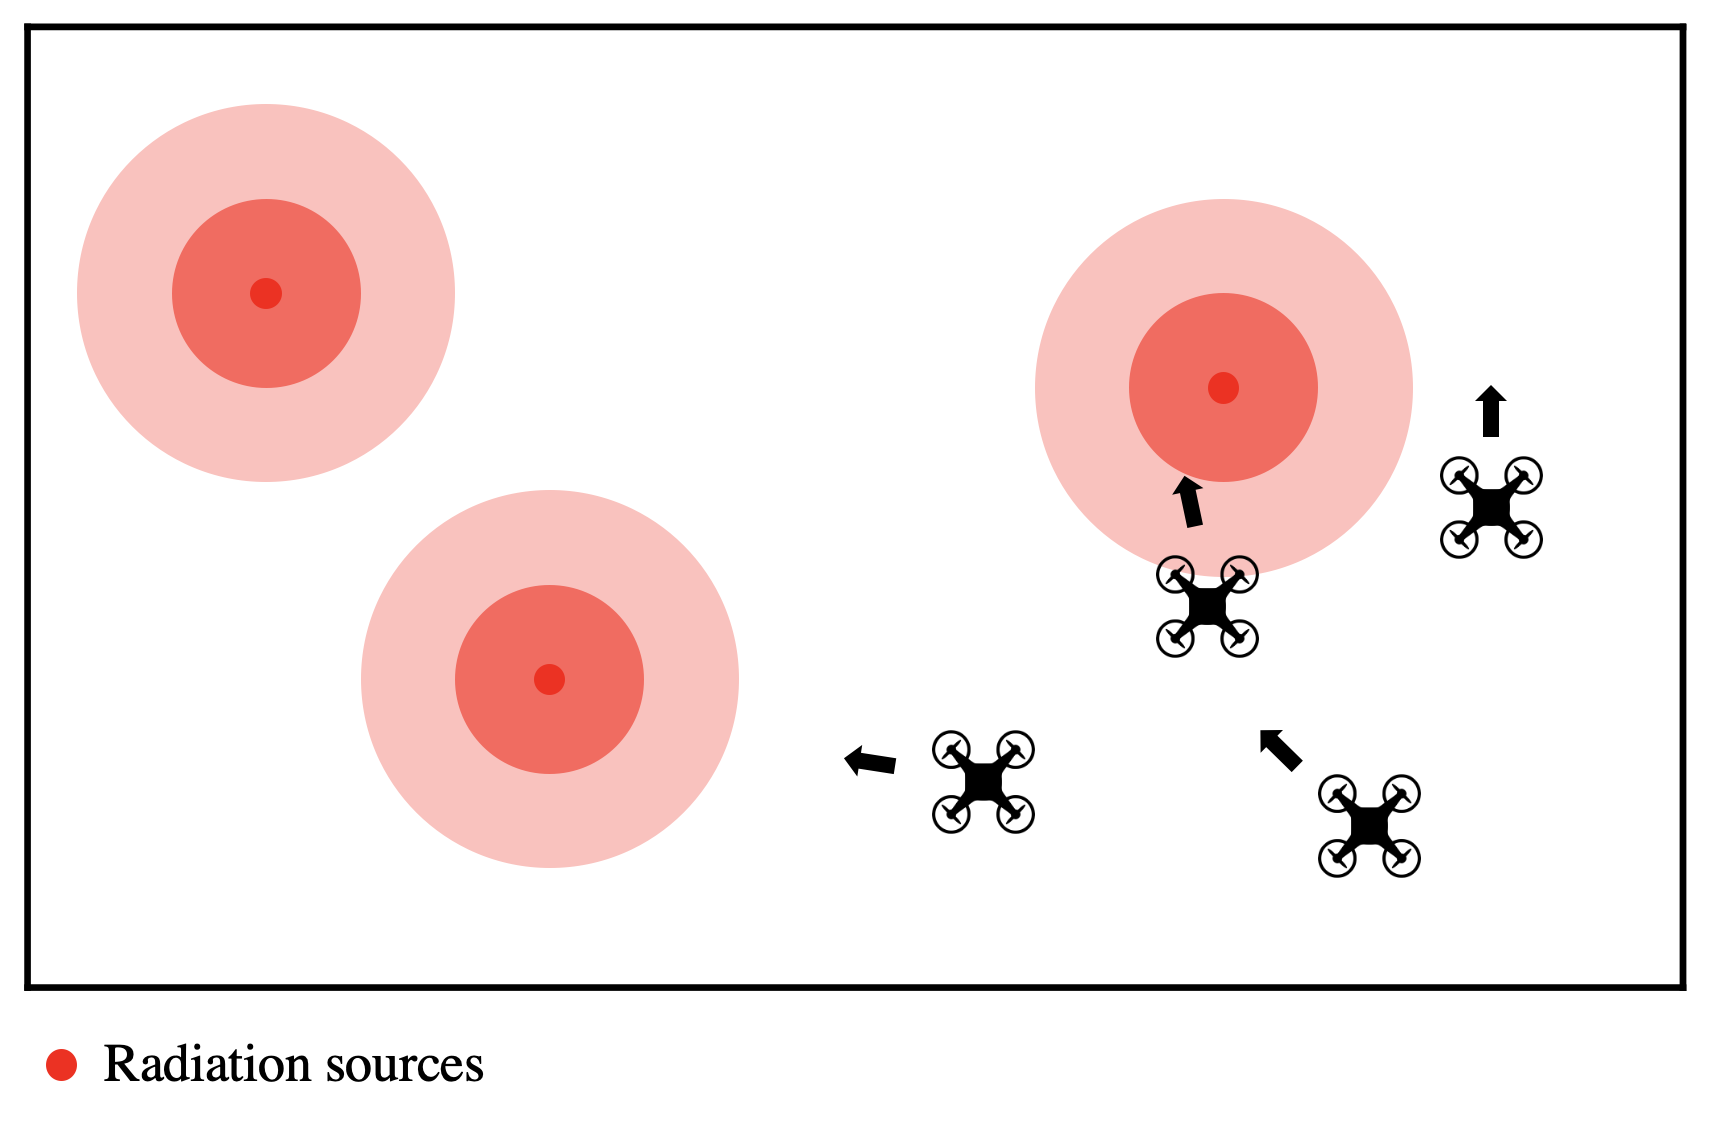
\includegraphics[width=\textwidth]{images/risk_aware_a.png}
%     %      \caption{}
%     %      \label{risk_aware_a}
%     % \end{subfigure}
%     % \hfill
    
    
%     \begin{subfigure}{0.30\textwidth}
%          \centering
%          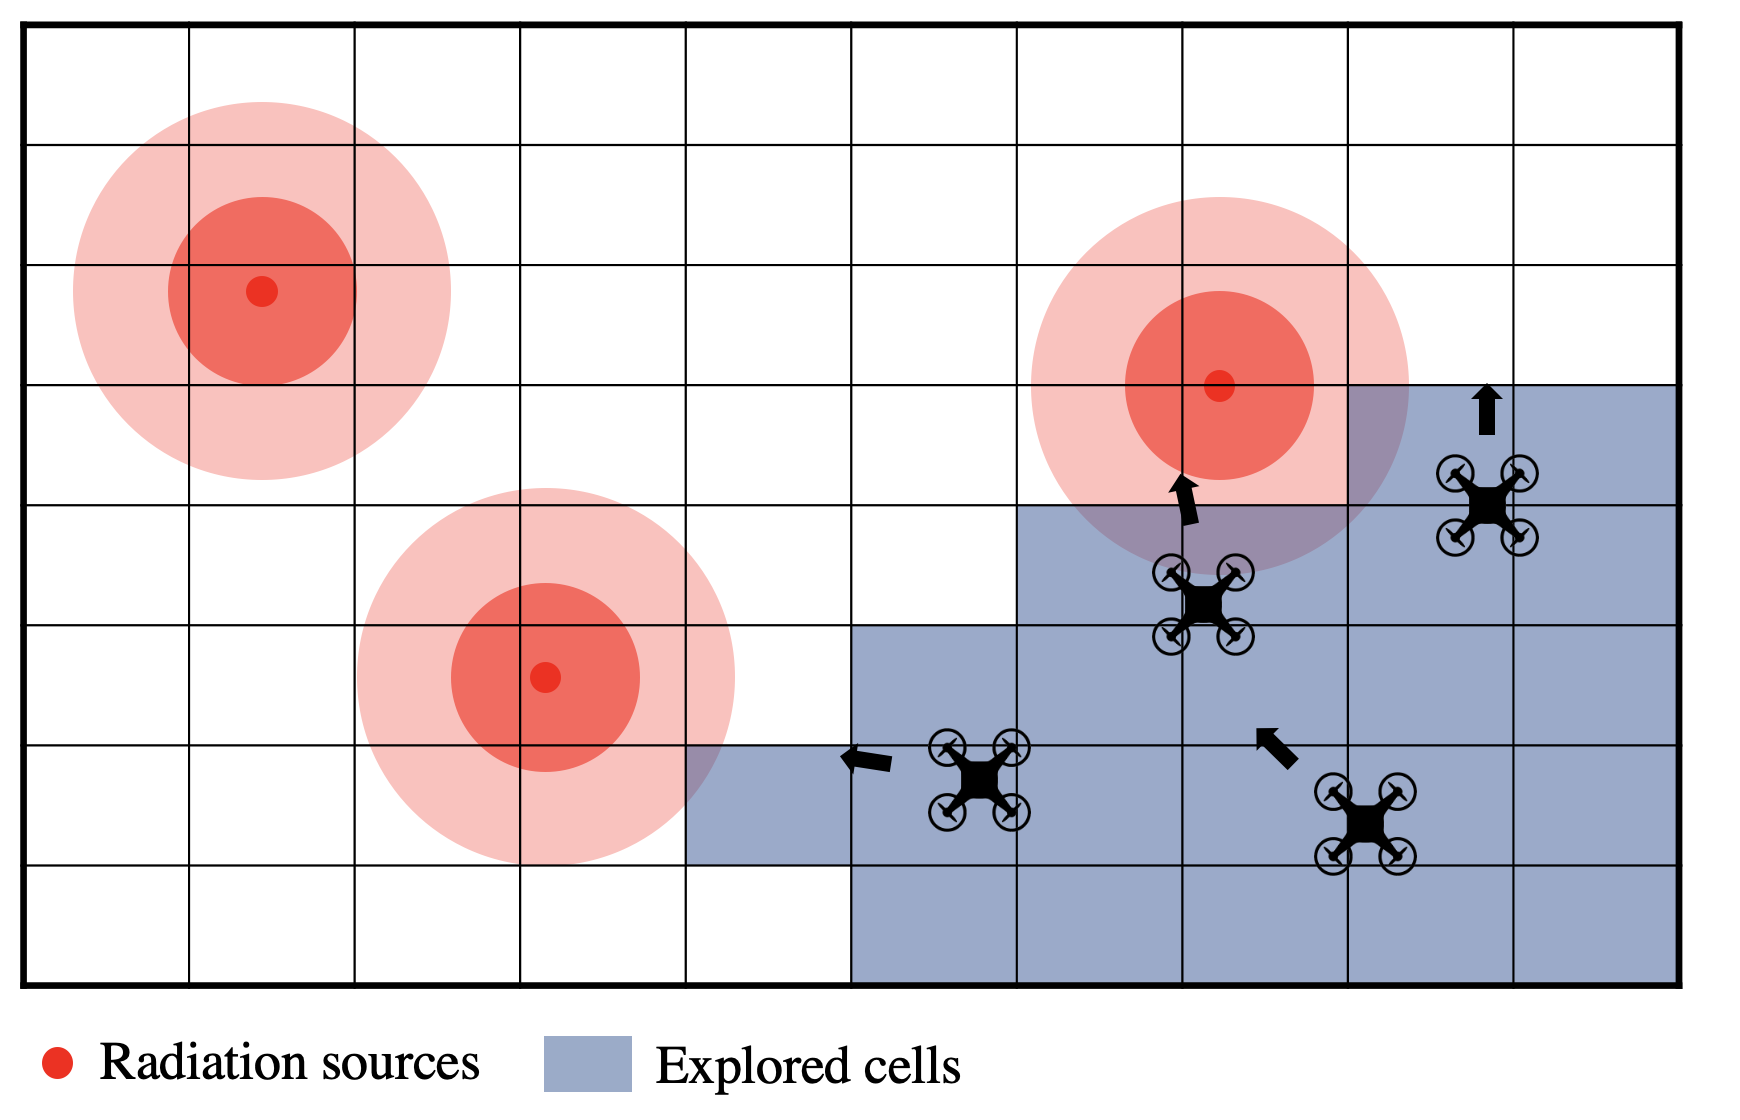
\includegraphics[width=\textwidth]{images/risk_aware_b.png}
%          \caption{}
%          \label{risk_aware_b}
%     \end{subfigure}
%     \hfill
%     \begin{subfigure}{0.30\textwidth}
%          \centering
%          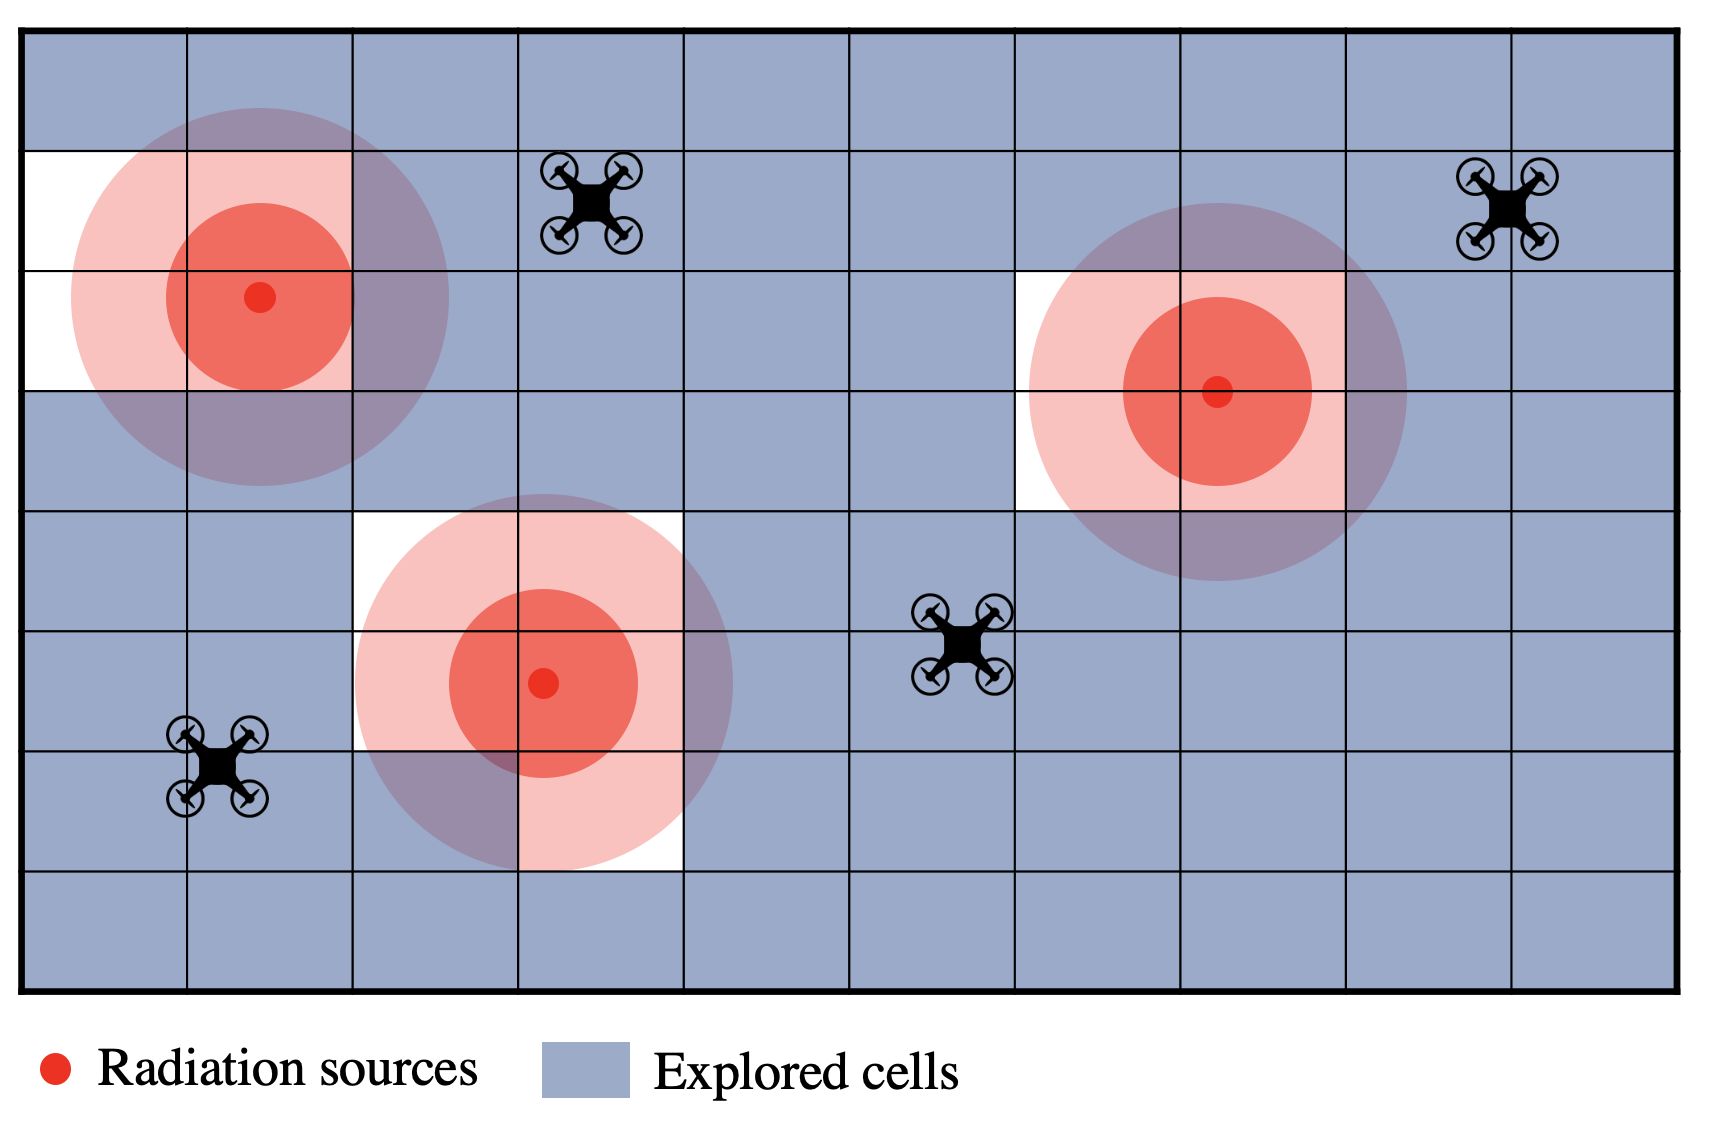
\includegraphics[width=\textwidth]{images/risk_aware_c.png}
%          \caption{}
%          \label{risk_aware_c}
%     \end{subfigure}
%     \hfill
%     \begin{subfigure}{0.30\textwidth}
%          \centering
%          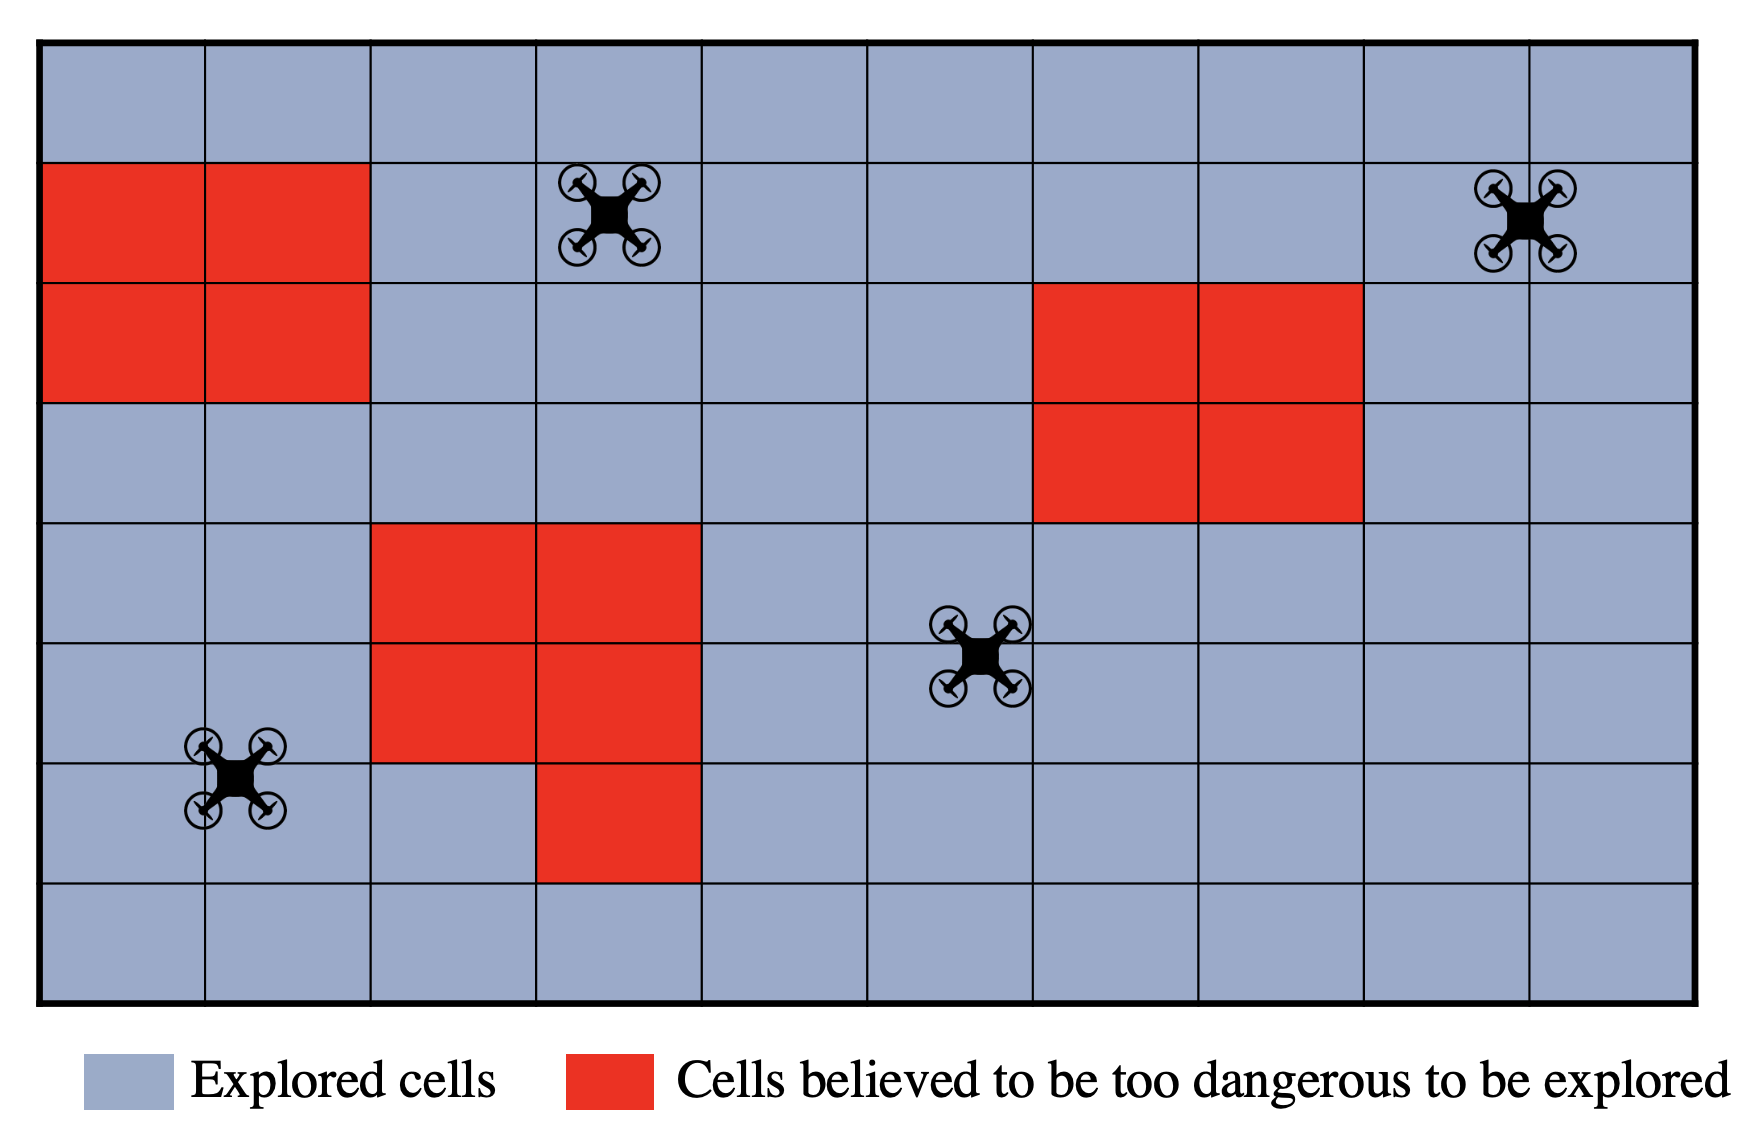
\includegraphics[width=\textwidth]{images/risk_aware_d.png}
%          \caption{}
%          \label{risk_aware_d}
%     \end{subfigure}
%         \caption{Risk aware exploration intuition. Fig. \ref{risk_aware_b}: Robots start exploring a hazardous environment. When a new cell is explored, the sensed radiation is used to update the DBM. Fig. \ref{risk_aware_c}: The cells have been mostly covered by the robots. Fig. \ref{risk_aware_d}: Only cells believed to be too dangerous remain unexplored.}
%     \label{risk_aware}
% \end{figure*}


\subsection{Risk Modelling}
Without loss of generality, we model risk considering point radiation
sources, denoted by the set $S$. The intensity of each radiation
source is given by $I_j\sim\mathcal{U}(0, 1)$. Each source's position
is denoted by $\bm{s}_j \in E$. Given a robot $a_i$'s discrete
position $\bm{x}_i \in E$, the perceived radiation level by that robot coming from radiation source $\bm{s}_j$ is given by:

\begin{equation}
    r_{\bm{s}_j}(\bm{x}_i) = \frac{I_j}{1 + \lambda\rho^2}
    \label{eq:radiation}
\end{equation}

which decays as the distance $\rho$ between $\bm{s}_j$ and $\bm{x}_i$
increases, and $\lambda$ is a decay constant. Measurement noise is
accounted for in the form of a Gaussian background radiation
$b \sim \mathcal{N}(0, 0.05)$. The total radiation perceived by a robot is:

\begin{equation}
    r(\bm{x}_i) = b + \sum_{\bm{s}_j \in S} r_{\bm{s}_j}(\bm{x}_i)
\end{equation}

Robots are only able to sense the radiation level associated with
their current position using an onboard sensor. They do not hold any
knowledge of where the radiations sources are located in the
environment. For the following definitions, it should be noted that
$r_{s_j}: E \rightarrow [0, 1]$.  Let
the event of robot $a_i$ failing be $f_i=1$, the probability of such a
failure due to an individual source of radiation follows a Bernoulli
distribution:
$\mathbb{P}(f_i = 1 | \bm{s}_j) \sim
\mathcal{B}(r_{\bm{s}_j}(\bm{x}_i))$. We assume that the sources of
radiation affect the robots independently, consequently the probability of a
robot failing due to the combined effect of all radiation sources is:

\begin{equation}
    \mathbb{P}(f_i = 1 | S) = 1 - \prod_{\bm{s_j} \in S} (1 - \mathbb{P}(f_i = 1 | \bm{s}_j))
    \label{eq:failure}
\end{equation}

\subsection{Information Modelling}
The objective of exploring an unknown dynamic environment is to gain
information about it. Moreover, this information should be as up to
date as possible. Therefore, it is unlikely that visiting a recently
explored cell will yield any significant gain as the information
should not have changed drastically. Conversely, exploring areas
visited long ago should yield a greater information gain, and
unvisited areas should provide the highest information gain. The last
time of exploration $t_\epsilon$ by robot $a_i$ of a cell at position
$\bm{x}_i$ can be represented by the scalar field
$\epsilon(\bm{x}_i) = t_\epsilon$. Let $u_i=1$ be the event of robot
$a_i$ finding useful information in a cell and
$\Delta t = t-t_\epsilon$ the time elapsed since the cell was last
visited, with $t$ being the current time. Then, the probability of
\textit{not} finding useful information
$\mathbb{P}(u_i=0 | f_i=0, \Delta t)$ can be modelled as an
exponential distribution with the following probability density
function:

\begin{equation}
    f(\Delta t;\omega) = \omega e^{-\omega\Delta t}
    \label{eq:information}
\end{equation}

where $\omega$ is the rate parameter of the distribution. In words,
the longer the cell has not been visited, the higher the chance
something has changed and consequently the lower the chance of not
finding useful information. Intuitively, no information can be acquired by failed robots.

\subsection{Distributed Belief Map}
To implement a DBM, we use the virtual
stigmergy~\cite{pinciroliTuple2016} from the
Buzz~\cite{pinciroliBuzz2016} programming language. Because
$r(\bm{x}_i)$ and $\epsilon(\bm{x}_i)$ are both scalar fields, they
lend themselves particularly well to being stored in a CRDT at a low
cost. At each time step, the robots store their values of
$r(\bm{x}_i)$ and $\epsilon(\bm{x}_i)$ in their respective
stigmergies.  The inputs to both fields are used as keys in the distributed belief map (more precisely, a concatenation of $\bm{x}_{i;x}$ and $\bm{x}_{i;y}$). This
means that the cost of storing the information for a given time step
is very low, especially as the keys consist of a few characters and
the values are floating point numbers. Storing the information into
the DBM via the virtual stigmergy allows robots to share their
observations as it is accessible by every robot in the system. Thus, a
robot visiting a cell for the first time could still have information from
which to compute a good control policy if this cell was previously
visited by another robot. In the event of a collision in the stigmergy
(when robots write to the same key in the same $t$), the robot making the latest observation updates the table. When a robot writes to a key already present
in the stigmergy (from a previous time step), the new data is merged
with an average and the result is propagated. A running average was used to update the belief map because of the noisy readings. 

\subsection{Control Law}
We assume that robots can be controlled through a position-based
control law. The best control policy should attempt to minimize
probability of failure and to maximize information gain. While the
directions achieving these individual objectives might be at odds in
the short term, they are in fact complementary in the long term
because no information can be gained if a robot failed, which means that avoiding danger
implicitly leads to more opportunities of gaining information
\cite{schwagerMultirobotControlPolicy2017}.

\begin{figure}[h]
	\centering
    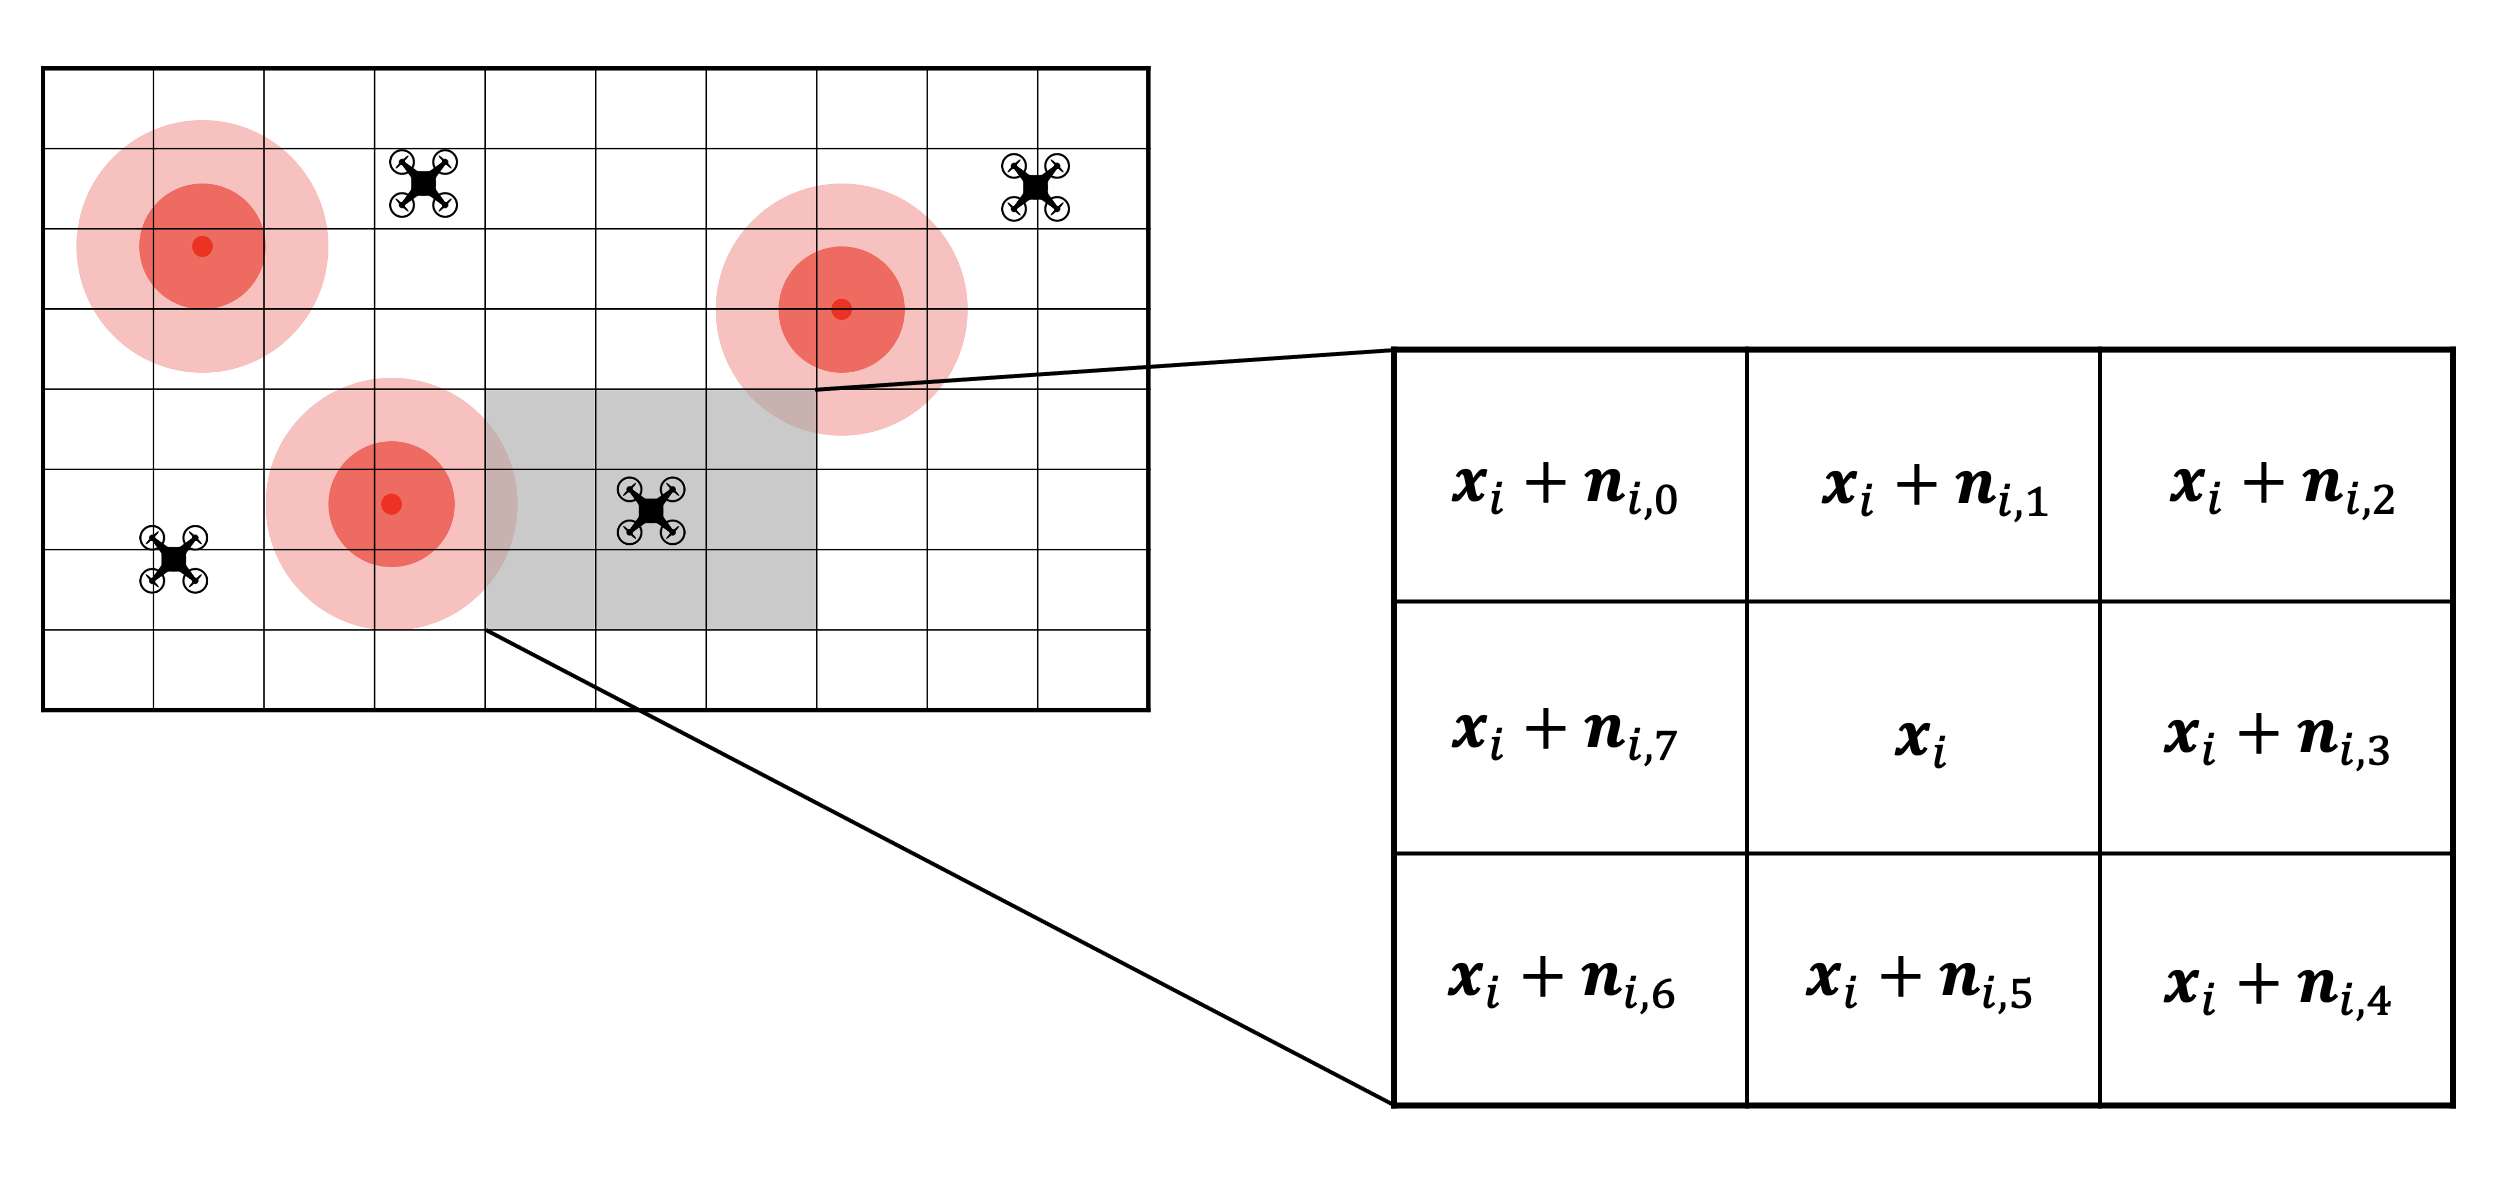
\includegraphics[width=0.95\columnwidth]{images/Moore.png}
    \caption{$\bm{x}_i$'s neighborhood. $\bm{n}_{i,0} = (-1, 1)$ is neighbor 0's offset from $\bm{x}_i$.}
    \label{neighborhood}
\end{figure}

For a robot at a given position $\bm{x}_i$, the directions where the
risk is minimized and the information gain is maximized are
respectively $\bm{\nabla}r(\bm{x}_i)$ and
$\bm{\nabla}\epsilon(\bm{x}_i)$, also denoted as $\bm{\nabla}_{r;i}$
and $\bm{\nabla}_{\epsilon;i}$. Calculating these globally at every
time step is too computationally expensive
\cite{dames2012decentralized,schwagerMultirobotControlPolicy2017}. Instead,
we compute them locally in a Moore neighborhood $\nu$ centered on
$\bm{x}_i$ as shown in Fig. \ref{neighborhood} where each neighboring
cell $\bm{n}_{i,j} \in \nu$ is a vector in $\mathbb{Z}^2$ representing
an offset from $\bm{x}_i$. We then have:

\begin{equation}
    \bm{\nabla}_{r;i} = \sum_{\bm{n}_j \in \nu}\frac{\partial r}{\partial \bm{n}_{i,j}} \bm{\hat{n}}_{i,j} \text{ , with } \frac{\partial r}{\partial \bm{n}_{i,j}} = r(\bm{x}_i) - r(\bm{n}_{i,j})
    \label{eq:gradient_risk}
\end{equation}

\begin{equation}
    \bm{\nabla}_{\epsilon;i} = \sum_{\bm{n}_j \in \nu}\frac{\partial \epsilon}{\partial \bm{n}_{i,j}} \bm{\hat{n}}_{i,j} \text{ , with } \frac{\partial \epsilon}{\partial \bm{n}_{i,j}} = \epsilon(\bm{x}_i) - \epsilon(\bm{n}_{i,j})
    \label{eq:gradient_exploration}
\end{equation}

% \begin{equation}
%     \frac{\partial r}{\partial \bm{n}_{i,j}} = r(\bm{x}_i) - r(\bm{n}_{i,j})
%     \label{eq:neighbor}
% \end{equation}

% \begin{equation}
%     \bm{\nabla}_{r;i} = \sum_{\bm{n}_j \in \nu}\frac{\partial r}{\partial \bm{n}_{i,j}} \bm{\hat{n}}_{i,j}
%     \label{eq:gradient}
% \end{equation}

% \begin{equation}
%     \frac{\partial \epsilon}{\partial \bm{n}_{i,j}} = \epsilon(\bm{x}_i) - \epsilon(\bm{n}_{i,j})
%     \label{eq:neighbor}
% \end{equation}

% \begin{equation}
%     \bm{\nabla}_{\epsilon;i} = \sum_{\bm{n}_j \in \nu}\frac{\partial \epsilon}{\partial \bm{n}_{i,j}} \bm{\hat{n}}_{i,j}
%     \label{eq:gradient}
% \end{equation}

where $\bm{\hat{n}}$ is the unit form of $\bm{n}$. Neighboring cells that have never been visited before are simply ignored when determining the gradients. If none of the neighboring cells have been explored yet, or if the computed direction is null, the robot simply moves forward until it's able to compute a meaningful direction. The movement vector $\bm{m}_i \in \mathbb{R}^2$ for the next time step
gives a good approximation for short term trajectory planning and is given by:

\begin{equation}
    \bm{m}_i = \alpha\bm{\nabla}_{r;i} + \beta\bm{\nabla}_{\epsilon;i} + \gamma\bm{o}_i
    \label{eq:movement}
\end{equation}

where $\alpha, \beta, \gamma$ are respectively the risk avoidance,
exploration and obstacle avoidance control gains. The parameters can
be adjusted arbitrarily; setting them to zero removes the effect
of the corresponding control law. The obstacle avoidance vector was
included to insure robustness and is taken from
\cite{shahriari2018lightweight}. With $\bm{\hat{m}_i}$ being the
normalized vector movement and $k$ a speed constant, the control law
for an agent $a_i$ at time step $t$ is expressed as:

\begin{equation}
    \bm{x}_i^{t+1} = \bm{x}_i^t + k \bm{\hat{m}}_i^t
    \label{eq:control}
\end{equation}

A constant search speed enables a fair comparison with the baselines detailed in section \ref{experimentSetup} as the exploration capabilities of the robots remain the same across the algorithms.

% \subsection{Implementation}
% The DBMs and the control law previously described are combined to create the behavior of an agent. At every
% time step, the information from the DBMs is used to determine the
% agent's next movement. The DBMs are then updated with the new
% information gained. Global exploration efficiency emerges through the
% exchange of information through the stigmergies, but no explicit
% coordination is required otherwise. Unlike FBE algorithms, DORA-Explorer never
% stops exploring the environment even if all cells are covered, as
% information could be gained by visiting "old" cells. If
% $\|\bm{\hat{m}}_i\|$ is too small, the agents move forward to avoid
% stagnation.

% \begin{algorithm}[h]
% \small
% \SetAlgoLined
% \DontPrintSemicolon
%  $\bm{x} \leftarrow random\_coordinates$\;
%  \While{True}{
%   $\nabla_r, \nabla_e \longleftarrow (0, 0), (0, 0)$\;
%   \;
%   \For{$n \in \nu$}{
%     $\nabla_r \leftarrow \nabla_r + (r\_stig[\bm{x}] - r\_stig[\bm{n}]) \cdot normalize(\bm{n})$\;
%     $\nabla_e \leftarrow \nabla_e + (e\_stig[\bm{x}] - e\_stig[\bm{n}]) \cdot normalize(\bm{n})$\;
%   }
%   \;
%   $\bm{m} \leftarrow \alpha \cdot \nabla_r + \beta \cdot \nabla_e + \gamma \cdot compute\_avoidance(sensors)$\;
%   $\bm{x} \leftarrow \bm{x} + k \cdot normalize(\bm{m})$\;
%   $r\_stig[\bm{x}], e\_stig[\bm{x}] \leftarrow get\_radiation(), time()$\;
%  }
%  \caption{DORA-Explorer Execution Loop}
%  \label{alg:dora}
% \end{algorithm}


% \begin{figure*}
%      \centering
%      \begin{subfigure}{0.30\textwidth}
%          \centering
%          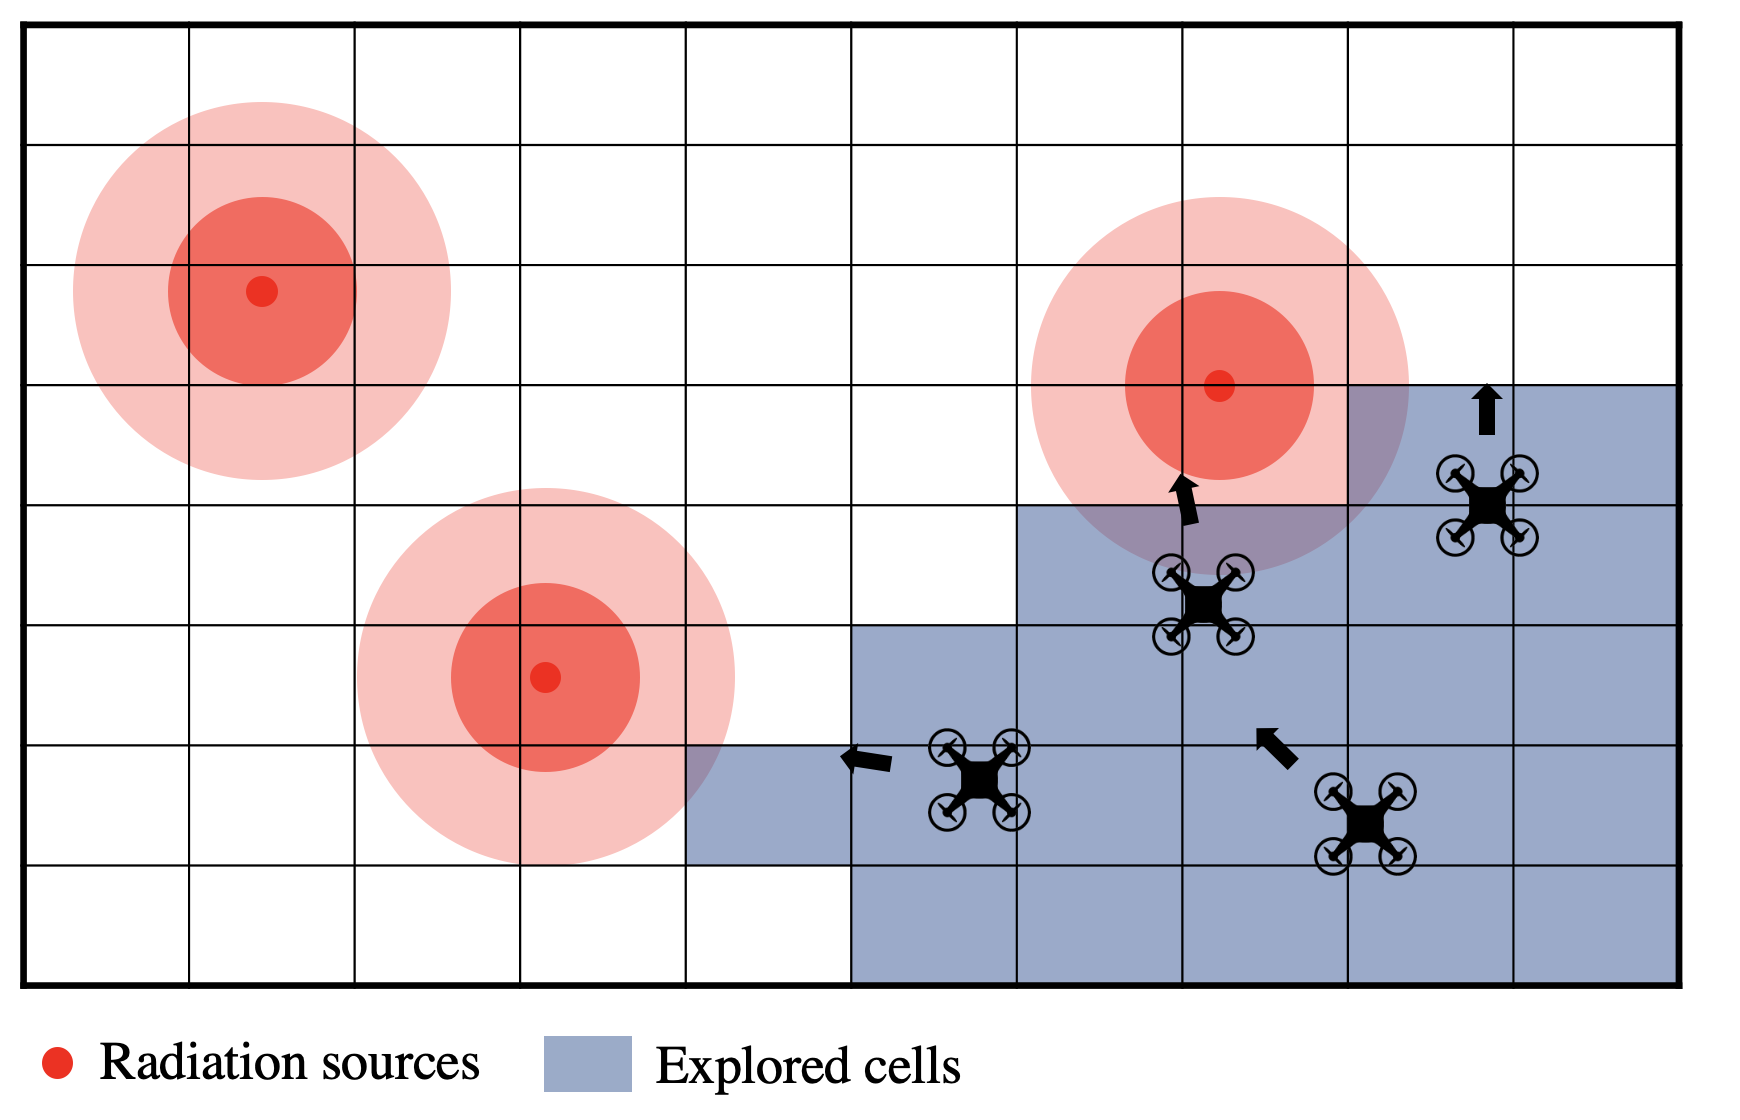
\includegraphics[width=\textwidth]{images/risk_aware_b.png}
%          \caption{}
%          \label{risk_unaware_a}
%      \end{subfigure}
%      \begin{subfigure}{0.30\textwidth}
%          \centering
%          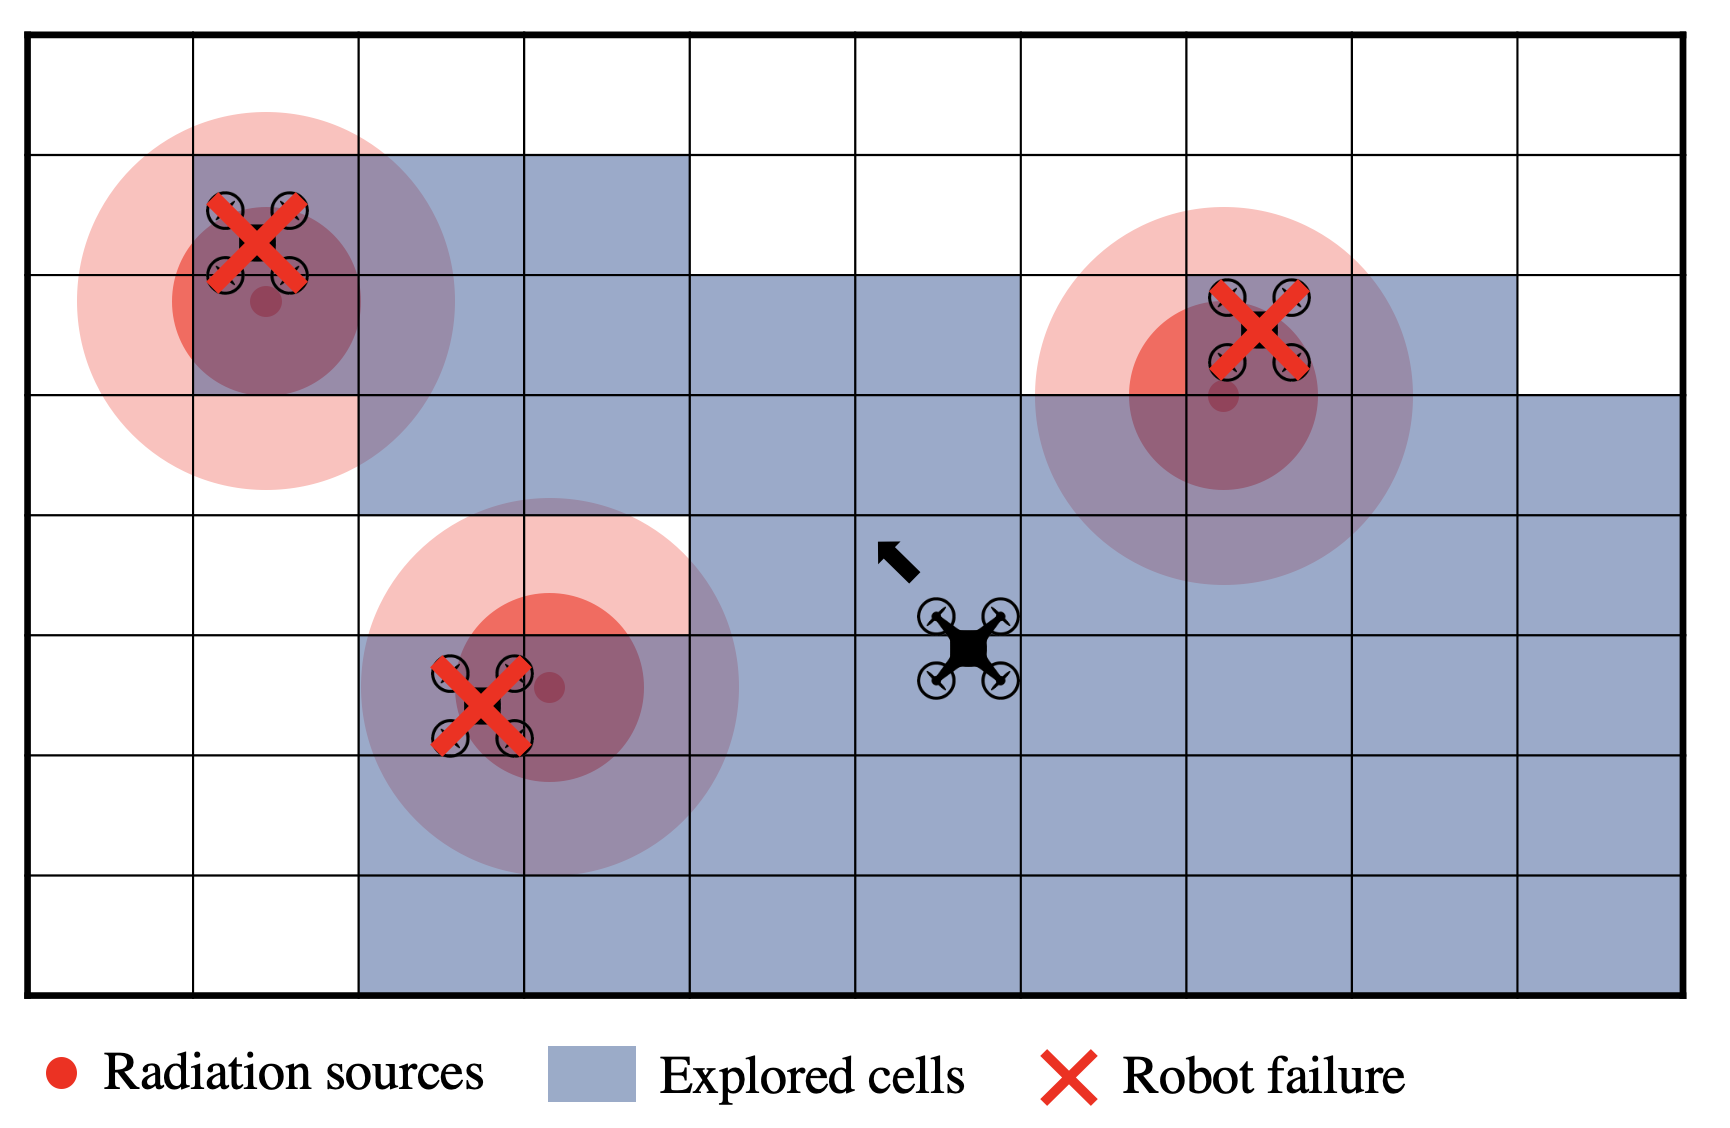
\includegraphics[width=\textwidth]{images/risk_unaware_a.png}
%          \caption{}
%          \label{risk_unaware_b}
%      \end{subfigure}
%         \caption{Exploration without risk awareness. Fig. \ref{risk_unaware_a}: Robots start exploring but are unable to sense environmental radiation. The only driving force of the algorithm is exploring new cells. Fig. \ref{risk_unaware_b}: Robots fail because they do not discriminate between safe and dangerous cells. Exploration is carried out fewer robots. Exploration efficiency drastically decreases and large areas of the environment remain uncovered.}
%         \label{risk_unaware}
% \end{figure*}

% \begin{figure*}[h]
%     \centering
%     % \begin{subfigure}{0.40\textwidth}
%     %      \centering
%     %      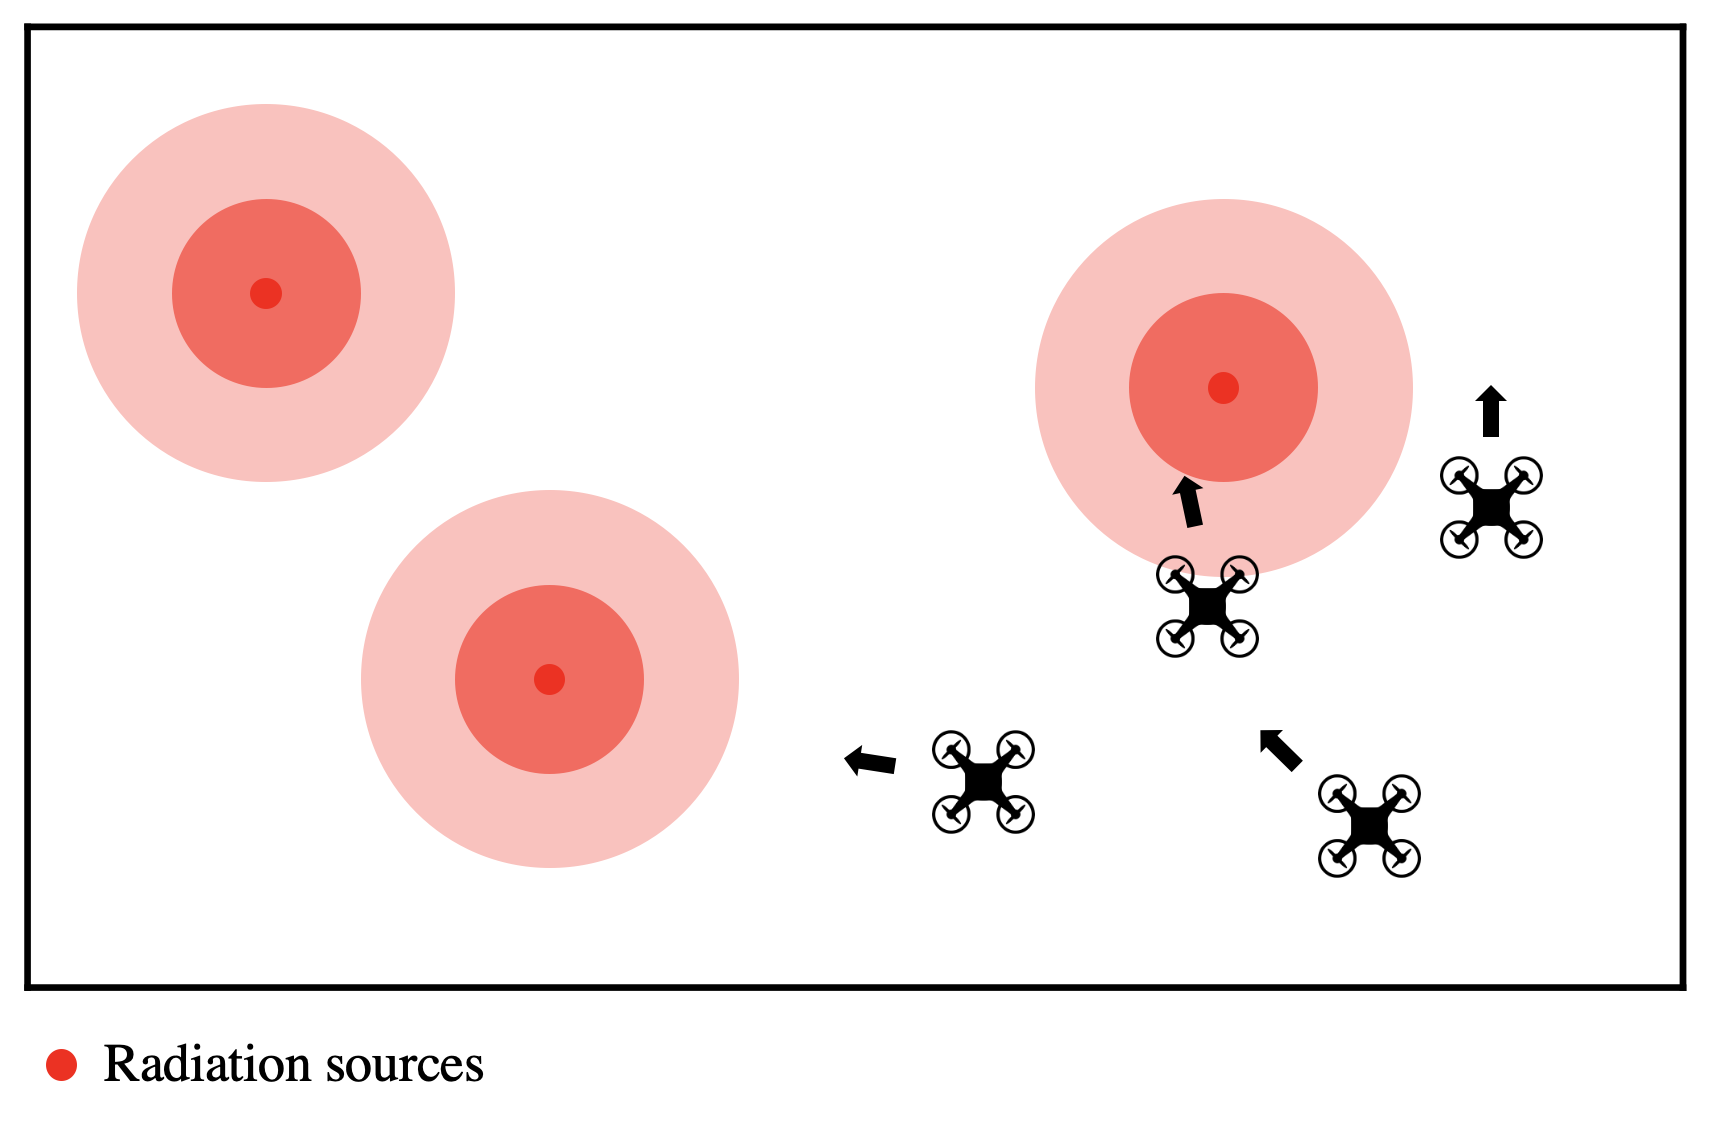
\includegraphics[width=\textwidth]{images/risk_aware_a.png}
%     %      \caption{}
%     %      \label{risk_aware_a}
%     % \end{subfigure}
%     % \hfill
%     \begin{subfigure}{0.30\textwidth}
%          \centering
%          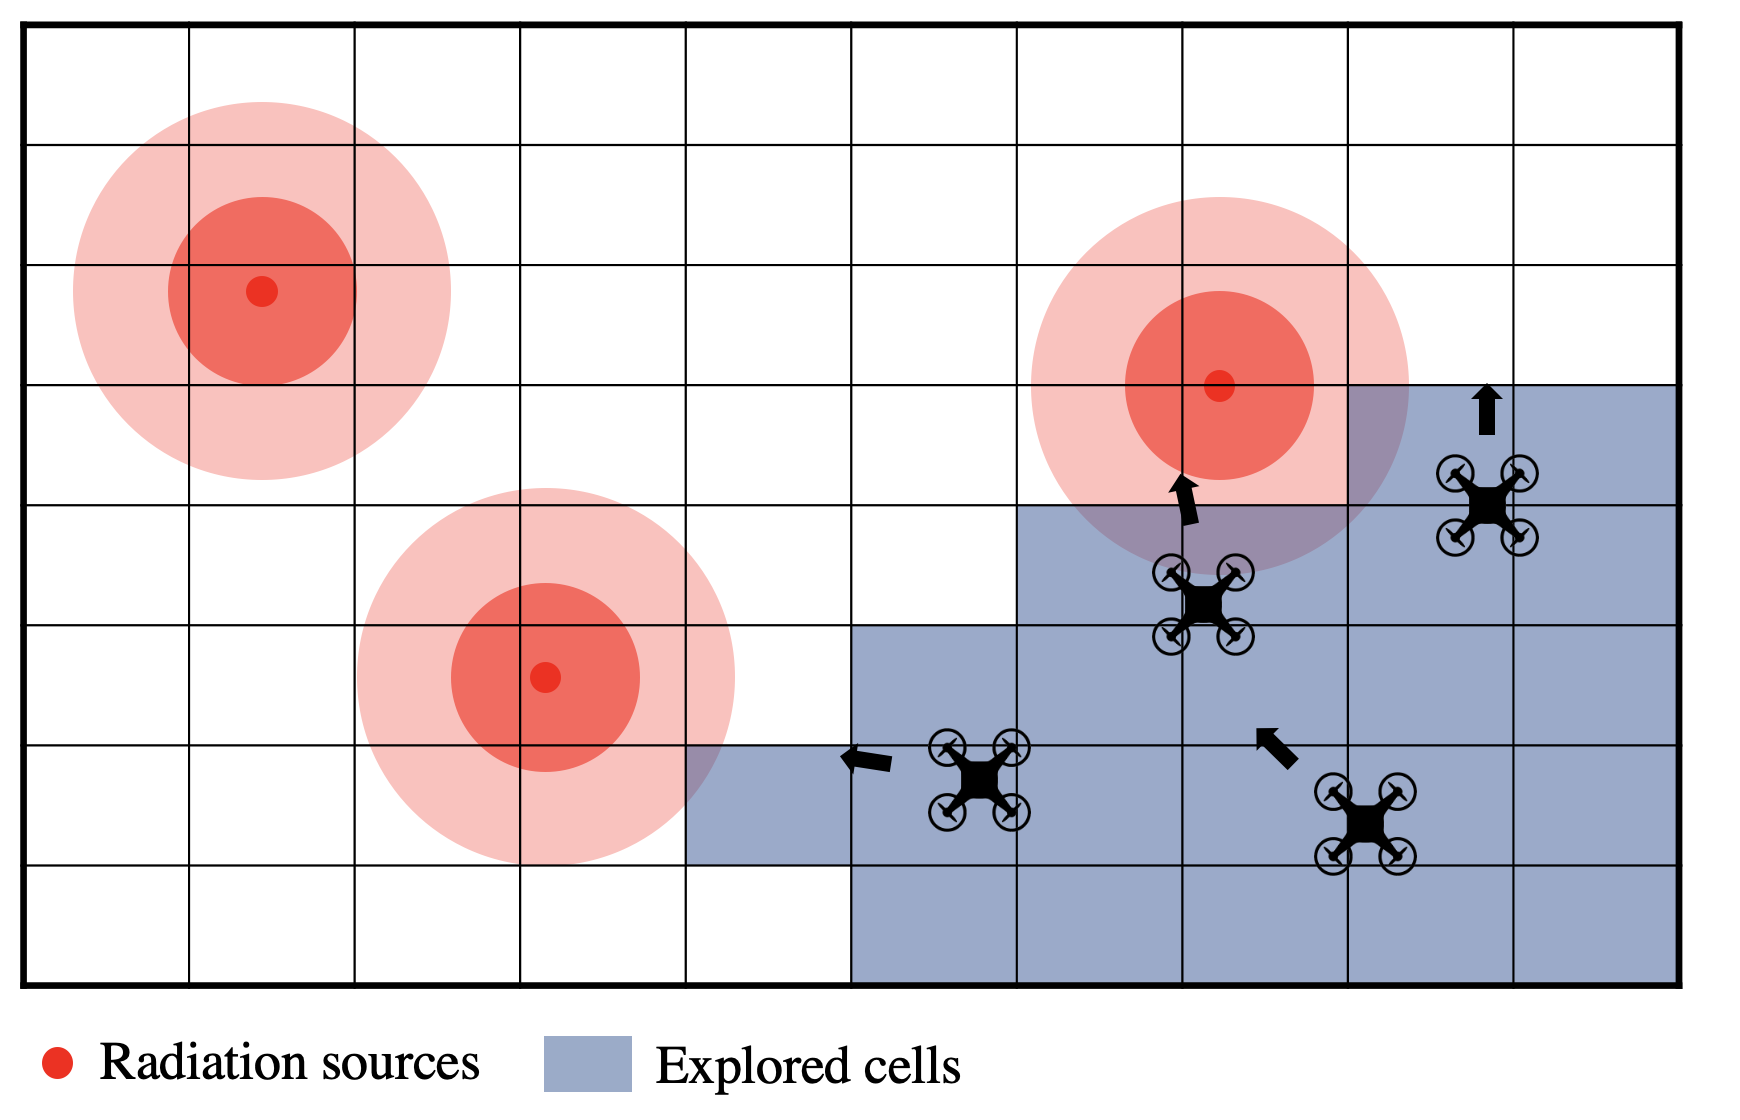
\includegraphics[width=\textwidth]{images/risk_aware_b.png}
%          \caption{}
%          \label{risk_aware_b}
%     \end{subfigure}
%     \hfill
%     \begin{subfigure}{0.30\textwidth}
%          \centering
%          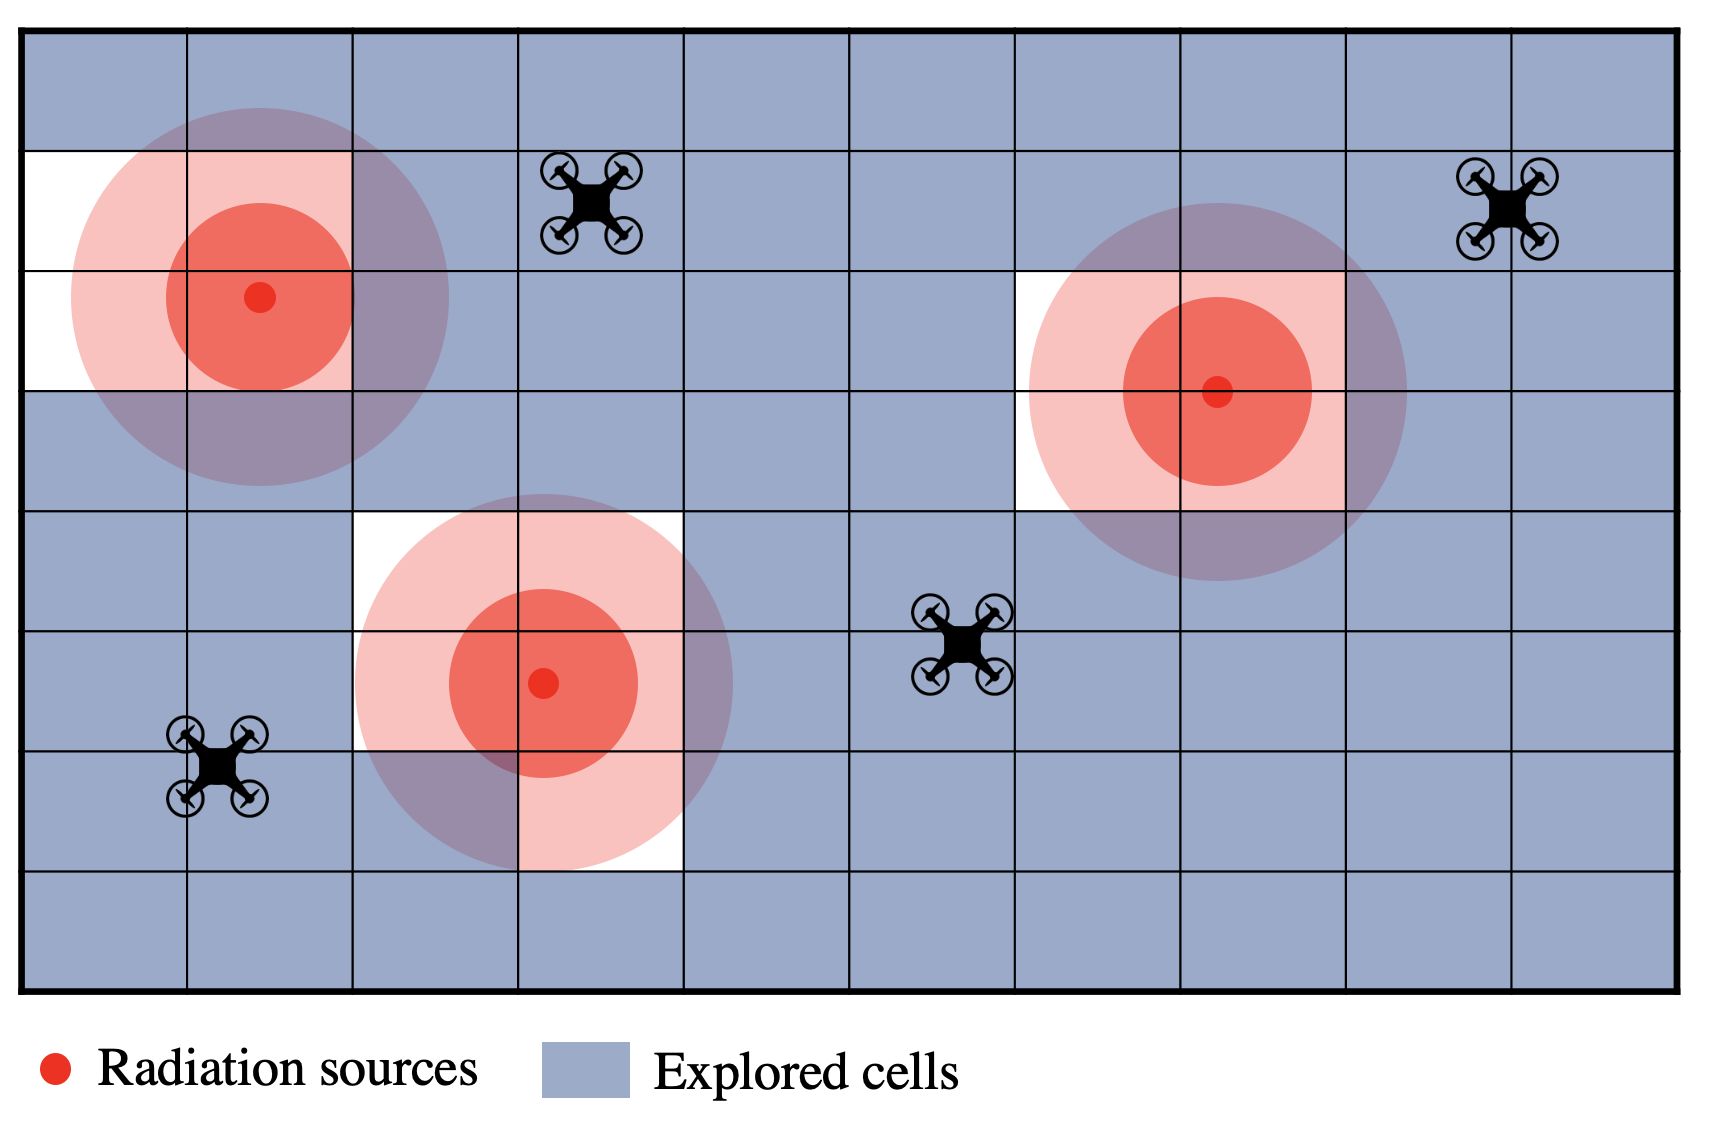
\includegraphics[width=\textwidth]{images/risk_aware_c.png}
%          \caption{}
%          \label{risk_aware_c}
%     \end{subfigure}
%     \hfill
%     \begin{subfigure}{0.30\textwidth}
%          \centering
%          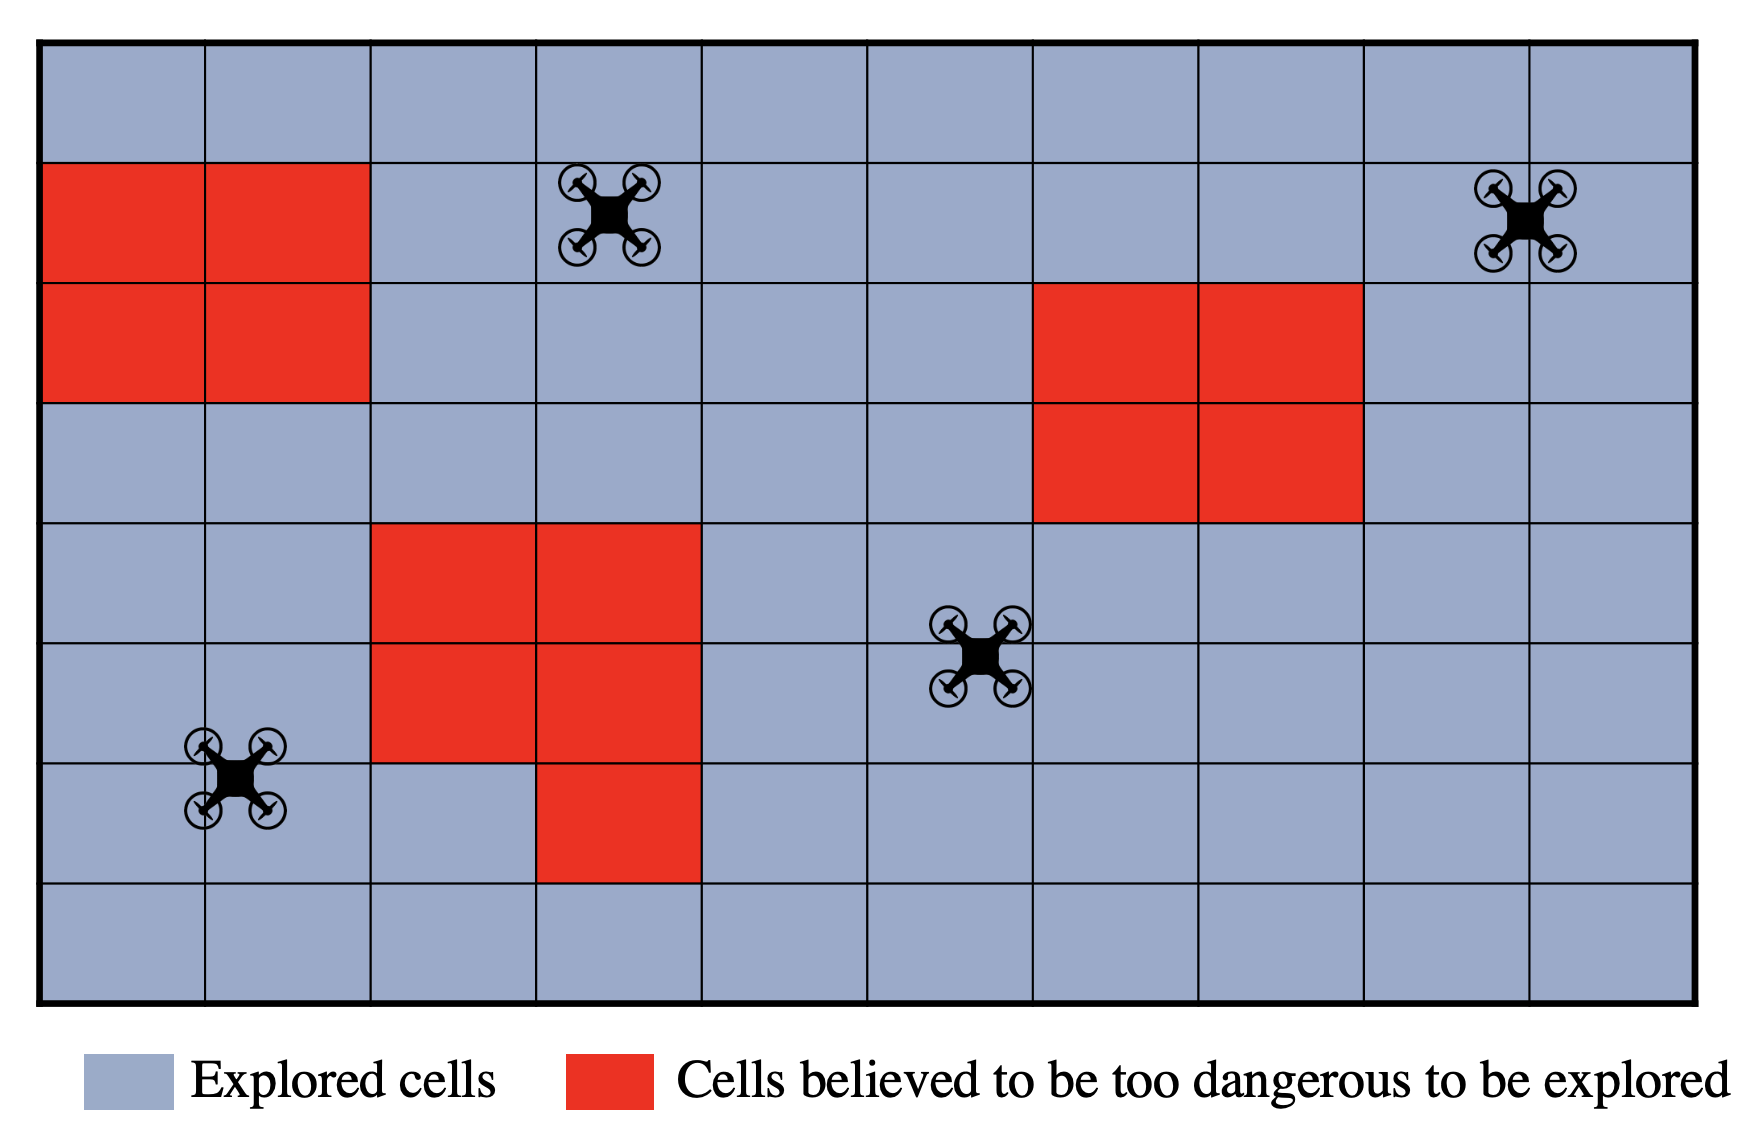
\includegraphics[width=\textwidth]{images/risk_aware_d.png}
%          \caption{}
%          \label{risk_aware_d}
%     \end{subfigure}
%         \caption{Risk aware exploration intuition. Fig. \ref{risk_aware_b}: Robots are dispatched in a hazardous environment and start exploring. When a new cell is explored by a robot, the sensed radiation is used to update the DBM. Fig. \ref{risk_aware_c}: The environment has been largely covered by the robots. Fig. \ref{risk_aware_d}: Only the cells believed to be too dangerous remain unexplored.}
%     \label{risk_aware}
% \end{figure*}

\subsection{Scalability}
\label{subsec:scalability}
To achieve scalability to a high number of agents and to large
environments, DORA-Explorer must have low communication and computational costs. Lowering the communication costs associated
with sharing the DBM can be done by using the virtual
stigmergy, which is designed to limit information exchange to read or
write operations only on the requested data. Because DORA-Explorer relies
solely on local information, the data transfer cost $D(A, \nu, E)$ for
an agent at a given time step is independent from the total number of
agents in $A$ and from the size of the environment $E$. For a
neighboring cell $\bm{n}_{i,j} \in \nu$, 2 stigmergy read operations
are needed per time step: one each to read $r(\bm{n}_{i,j})$ and
$\epsilon(\bm{n}_{i,j})$. In the same time step, the agent updates
$r(\bm{x}_i)$ and $\epsilon(\bm{x}_i)$ after it has moved to a new
location, which requires 2 stigmergy write operations. Each stigmergy
access requires only a few tens of bytes of data transfer for the key
and value. This mostly constant data quantity is represented as $d$,
we have $D(A, \nu, E) = 2d(|\nu| + 1)$. Similarly, the computational
cost $C(A, \nu, E)$ for the same agent at the same time step is kept
very low because of the reliance on local information only. Each time
step requires to compute 2 gradients, and referring to
\eqref{eq:gradient_risk}, \eqref{eq:gradient_exploration}, \eqref{eq:movement} and
\eqref{eq:control} we have that $C(A, \nu, E) = 12|\nu|+7$. The costs
related to $\bm{o}_i$ have been excluded from this analysis as
obstacle avoidance is not a critical part of DORA-Explorer. The step-wise communication
and computational costs for an agent are thus
both bounded by:

\begin{equation}
    D(A, \nu, E) \text{ and } C(A, \nu, E) \in \Theta(|\nu|)
    \label{eq:costs}
\end{equation}

Such low costs mean that DORA-Explorer should scale well to a large number of
robots and should enable real time computation on even very limited computational platforms.


\section{Simulations}
\subsection{Experimental setup}
\label{experimentSetup}

We tested our system through simulations in ARGoS
\cite{Pinciroli:SI2012}, which is an open-source physics-based
simulation environment designed for robotic swarms. The agents we used
in the simulation are KheperaIV robots 
\cite{kteam2021kheperaiv} programmed in Buzz \cite{pinciroliBuzz2016} to facilitate swarm
management and interaction. 

% These are small round robots (140mm of
% diameter) equipped with 8 infrared proximity sensors spread evenly
% around their frame to perform obstacle avoidance. The
% agents are programmed in Buzz to facilitate swarm
% management and interaction.

% \begin{figure}[h]
% 	\centering
%     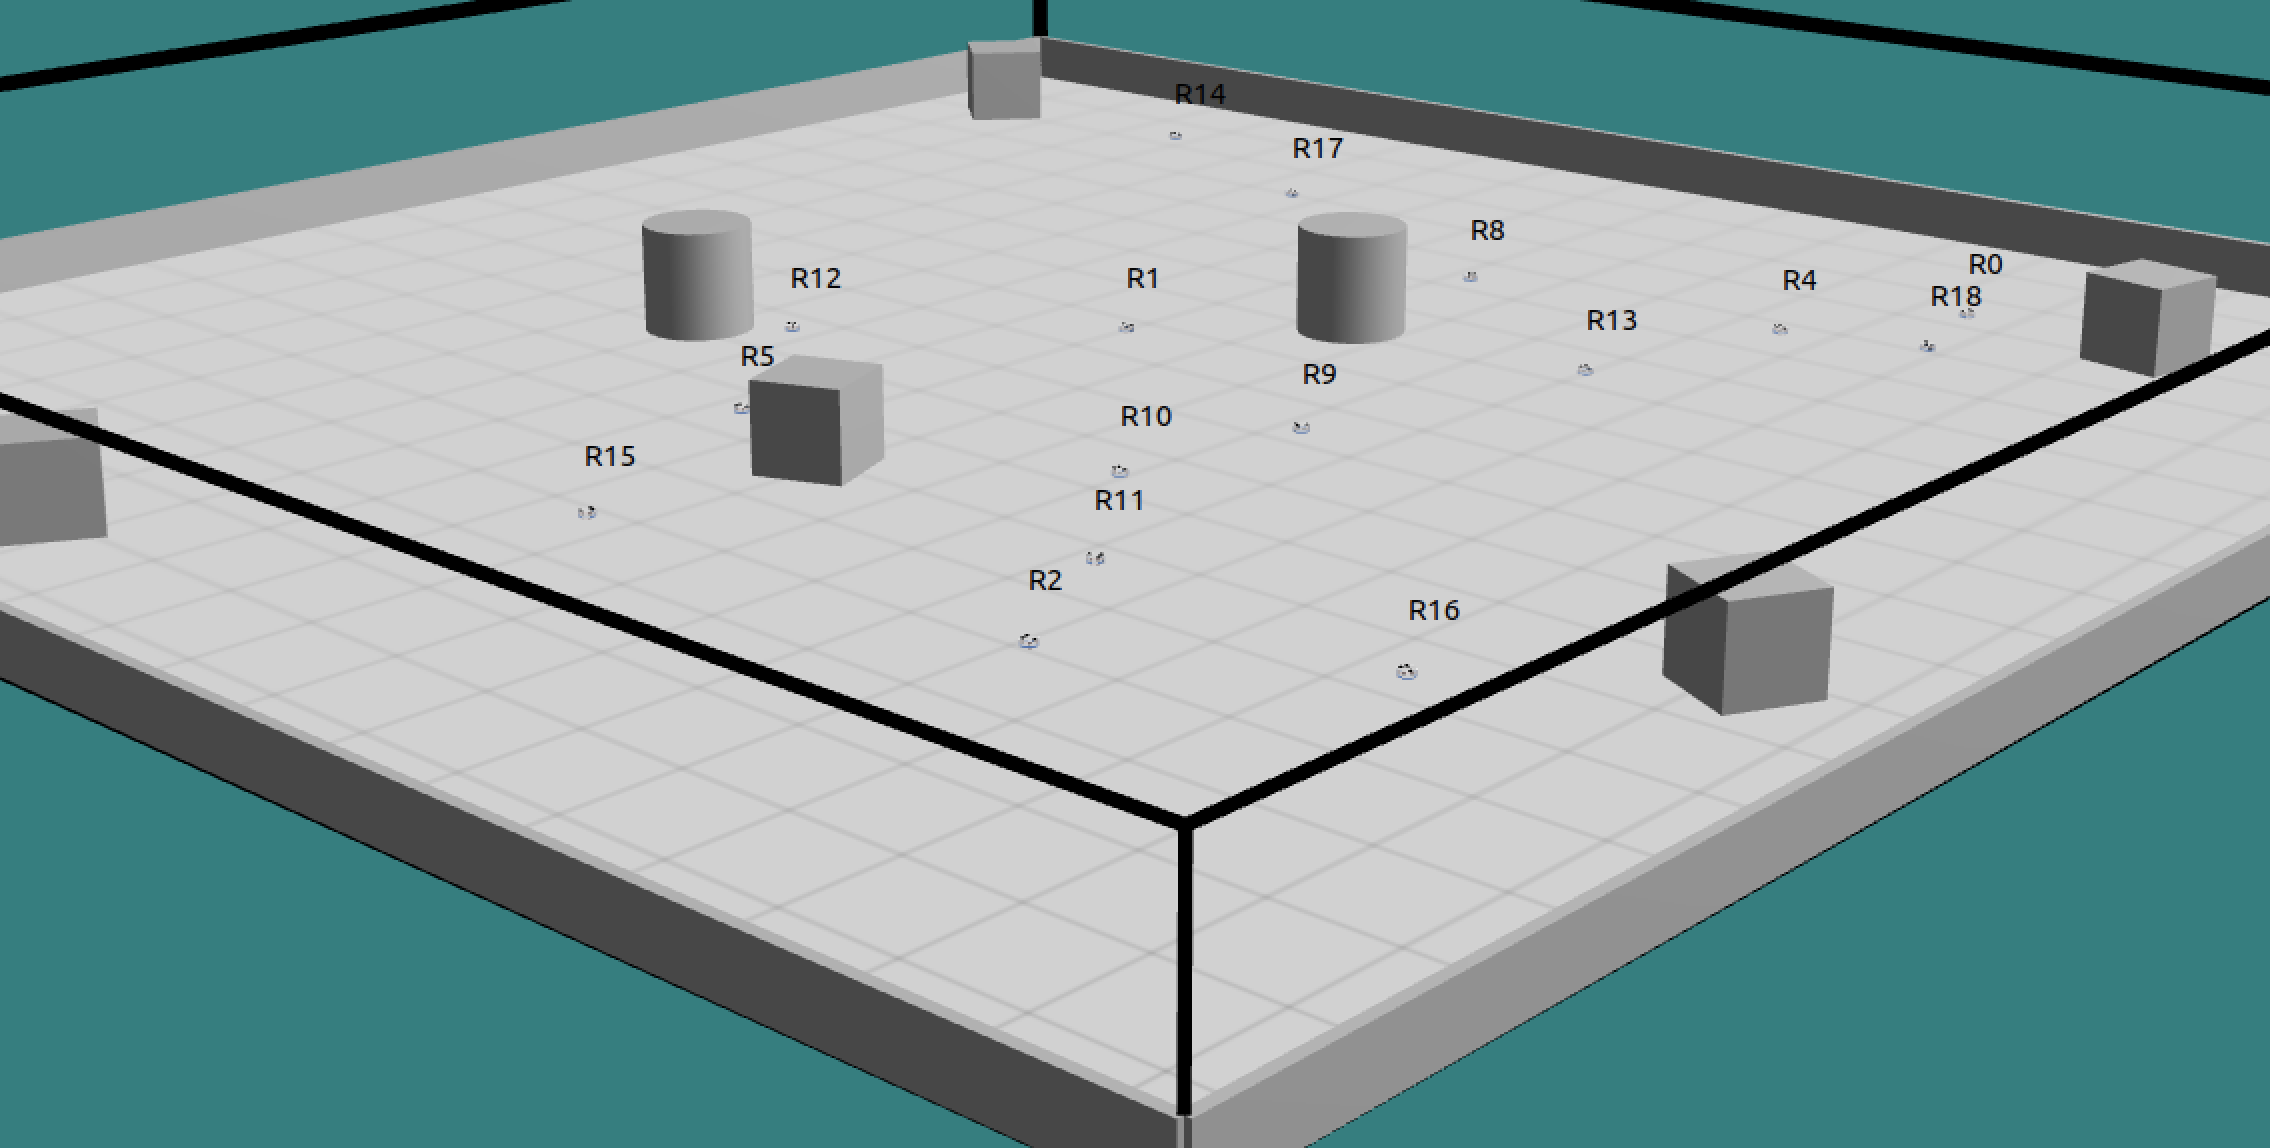
\includegraphics[width=0.95\columnwidth]{images/argos.png}
%     \caption{$400 \text{m}^2$ environment in the ARGoS simulator with 20 KheperaIV robots. Cylinders are radiation sources and boxes are random obstacles.}
%     \label{argos}
% \end{figure}

We deployed a set of N = \{10, 15, 20\} robots in a simulated
environment of 20x20m with set of 2 radiation sources. The environment is discretized into 400 cells, where each cell of the grid is 1x1m large. The robots'
initial positions are chosen randomly. We arbitrarily set $\lambda$ from
\eqref{eq:radiation} to be 5 as it was providing an adequate decay speed in relation with the size of our environment: The robots would generally fail in a 3m radius around the radiation sources. The speed constant $k$ from \eqref{eq:control} is set to
$20$ to match the maximal speed of the KheperaIV robots. Because no information gain can be achieved by a failed robot, failure must be avoided. This
leads to choosing $\alpha >= \beta$ in \eqref{eq:control}. For our
experiments, we set $\alpha=2, \beta=1$ and $\gamma=1$. The robots are
all given a random initial orientation. Radiation sensing is emulated
by an ARGoS controller reading the randomly generated radiation
sources. Failures are randomly triggered by using \eqref{eq:failure}:
if $f_i=1$, the robot stops exploring. We added 5 randomly distributed
0.8m x 0.8m obstacles to verify the robot's ability to
perform exploration even in cluttered environments.

% \begin{figure*}
%     \centering
%     \begin{subfigure}{0.32\textwidth}
%         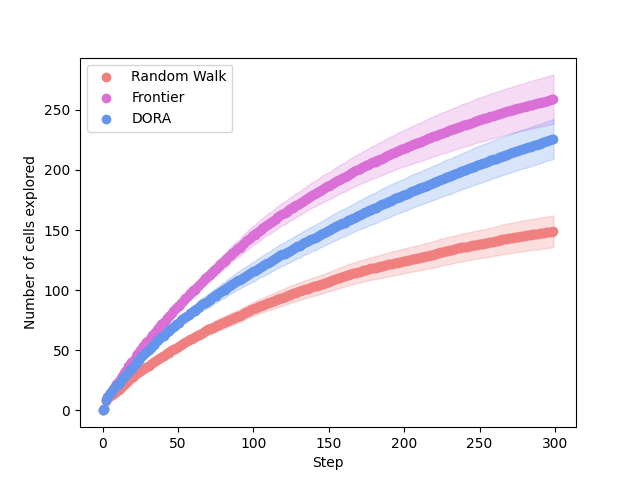
\includegraphics[width=\textwidth]{images/explored_10.png}
%         \caption{N=10 robots}
%         \label{results:explored10}
%     \end{subfigure}
%     \begin{subfigure}{0.32\textwidth}
%         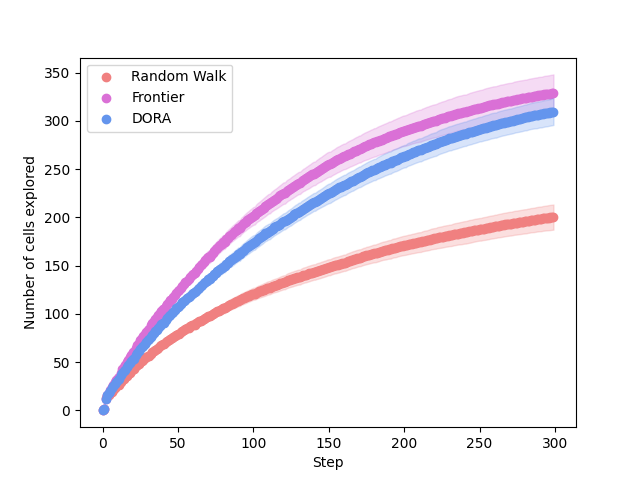
\includegraphics[width=\textwidth]{images/explored_15.png}
%         \caption{N=15 robots}
%         \label{results:explored15}
%     \end{subfigure}
%     \begin{subfigure}{0.32\textwidth}
%         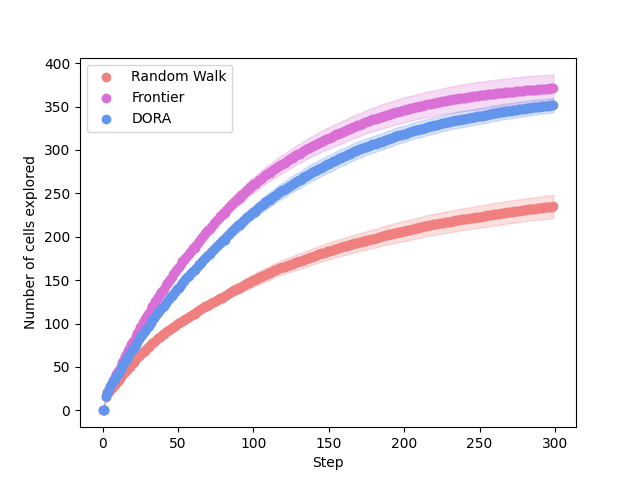
\includegraphics[width=\textwidth]{images/explored_20.png}
%         \caption{N=20 robots}
%         \label{results:explored20}
%     \end{subfigure}
%     \caption{Performance comparison of DORA-Explorer, FBE and random walk for number of explored cells over time.}
    
% \end{figure*}

% \begin{figure*}
%     \centering
%     \begin{subfigure}{0.32\textwidth}
%         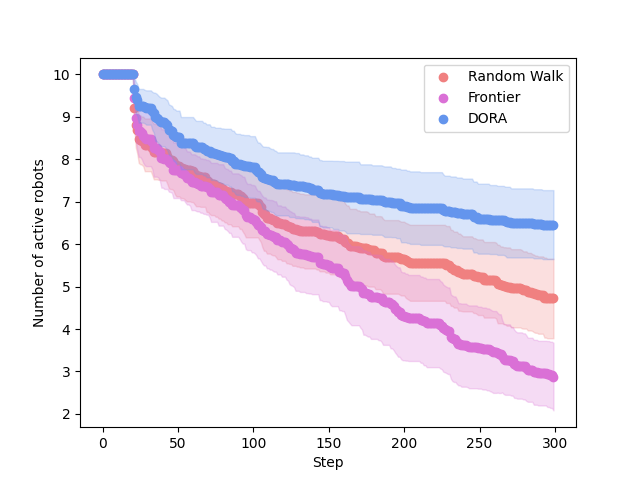
\includegraphics[width=\textwidth]{images/activerobots_10.png}
%         \caption{N=10 robots}
%         \label{results:failures10}
%     \end{subfigure}
%     \begin{subfigure}{0.32\textwidth}
%         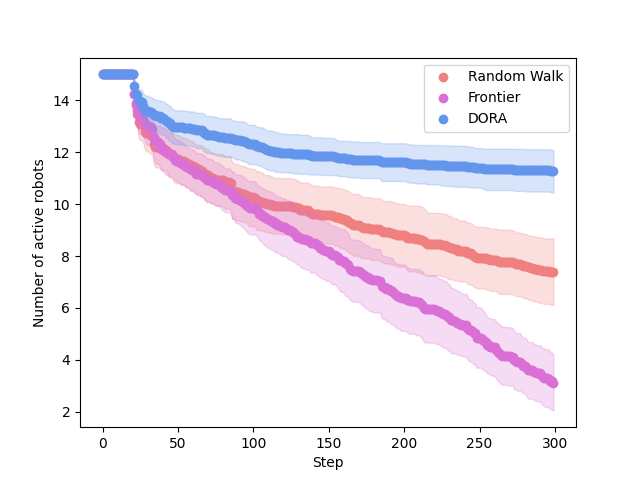
\includegraphics[width=\textwidth]{images/activerobots_15.png}
%         \caption{N=15 robots}
%         \label{results:failures15}
%     \end{subfigure}
%     \begin{subfigure}{0.32\textwidth}
%         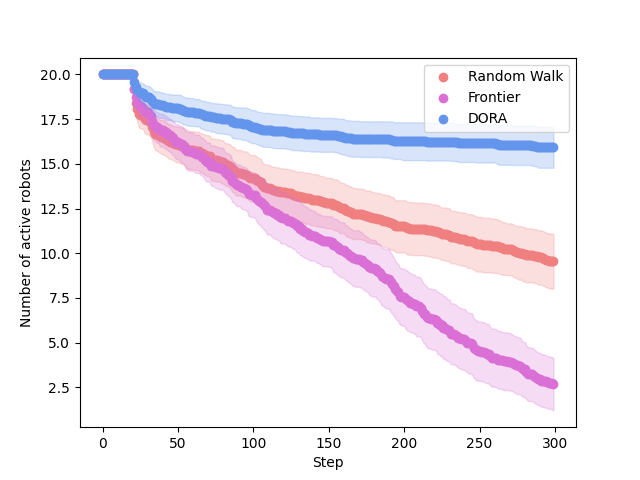
\includegraphics[width=\textwidth]{images/activerobots_20.png}
%         \caption{N=20 robots}
%         \label{results:failures20}
%     \end{subfigure}
%     \caption{Performance comparison of DORA-Explorer, FBE and random walk for number of active robots over time.}
% \end{figure*}



We performed 50 simulation runs over 300 steps of the DORA-Explorer
algorithm. Each time step lasts 0.8s. To assess DORA-Explorer's performance, we compare it to the results
obtained by a random walk algorithm and by a FBE algorithm. The
latter's key principle is to assign one of three states (explored,
frontier, unexplored) to the cells constituting the environment and to
coordinate the robots to explore the regions near the frontier. To
implement it, we adapted the algorithm from
\cite{yamauchi1998frontier} by having the robots share an exploration
map through a virtual stigmergy. The comparison with frontier exploration is
particularly relevant because it allows us to gain insights on our
algorithm performance in terms of terrain coverage compared to an
algorithm which was specifically designed to maximize this
objective. We also compare DORA-Explorer with a random walk algorithm as a
baseline it absolutely needs to outperform. These two baselines are
commonly used for the exploration of unknown environments in the field
of swarm robotics. They do not take risk into account, but to the best
of our knowledge, no other existing swarm exploration strategy does. To address this issue, we could have modified the baselines to take risk into account, but chose against it. Adding risk thresholds for movement could be considered. However, if the robots find themselves in radiation hotspots, they might remain stuck in these locations because all surrounding cells will a have similar/equal risk which is too high to allow movement, resulting in fatal stagnation. 

% Obstacle avoidance algorithms could have also been adapted to a risk avoidance context and serve as a baseline for DORA-Explorer. However, taking account of varying levels of risk would have been challenging. Again, it is hard to determine the threshold on risk level after which a cell should be considered as containing an obstacle.

% For the FBE method, a possibility would have been to treat radiation sources as obstacles and use an obstacle avoidance mechanism to stay away from them.
% However, there are two issues with this. First, these algorithms mostly focus on avoiding one obstacle at a time (the closest one), and therefore do not consider the effect of combined obstacles. This would not make sense anyway: two obstacles cannot be at the same location, while radiation sources can have a combined effect in one location. Second, these algorithms usually detect the presence of an obstacle in a binary way and are thus ill-suited for the presence of a gradual risk.

The first metric used to assess the validity of our approach is the
number of robots which remain active (not failed) over time. This is
perhaps the most important metric because it shows how well DORA-Explorer
performs in terms of risk avoidance, i.e. its main objective. The
second metric used to evaluate the algorithms is the total number of
cells explored by the swarm. This allows us to evaluate how well our
algorithm performs in its objective of maximizing information gain and
to verify that avoiding risk does not impact too much the exploration
performance. The third metric we studied is the communication costs of
the algorithms, measured in KB of data transmitted per robot at
each time step. We included this in our analysis to examine if
the algorithms can scale to large number of robots. We also ran simulations to study the impact of the parameters $\alpha$ and $\beta$ from (\ref{eq:movement}). 


\subsection{Results}

The following results are an average of the 50 simulation runs of each algorithm. 

\begin{figure}[]
    \centering
    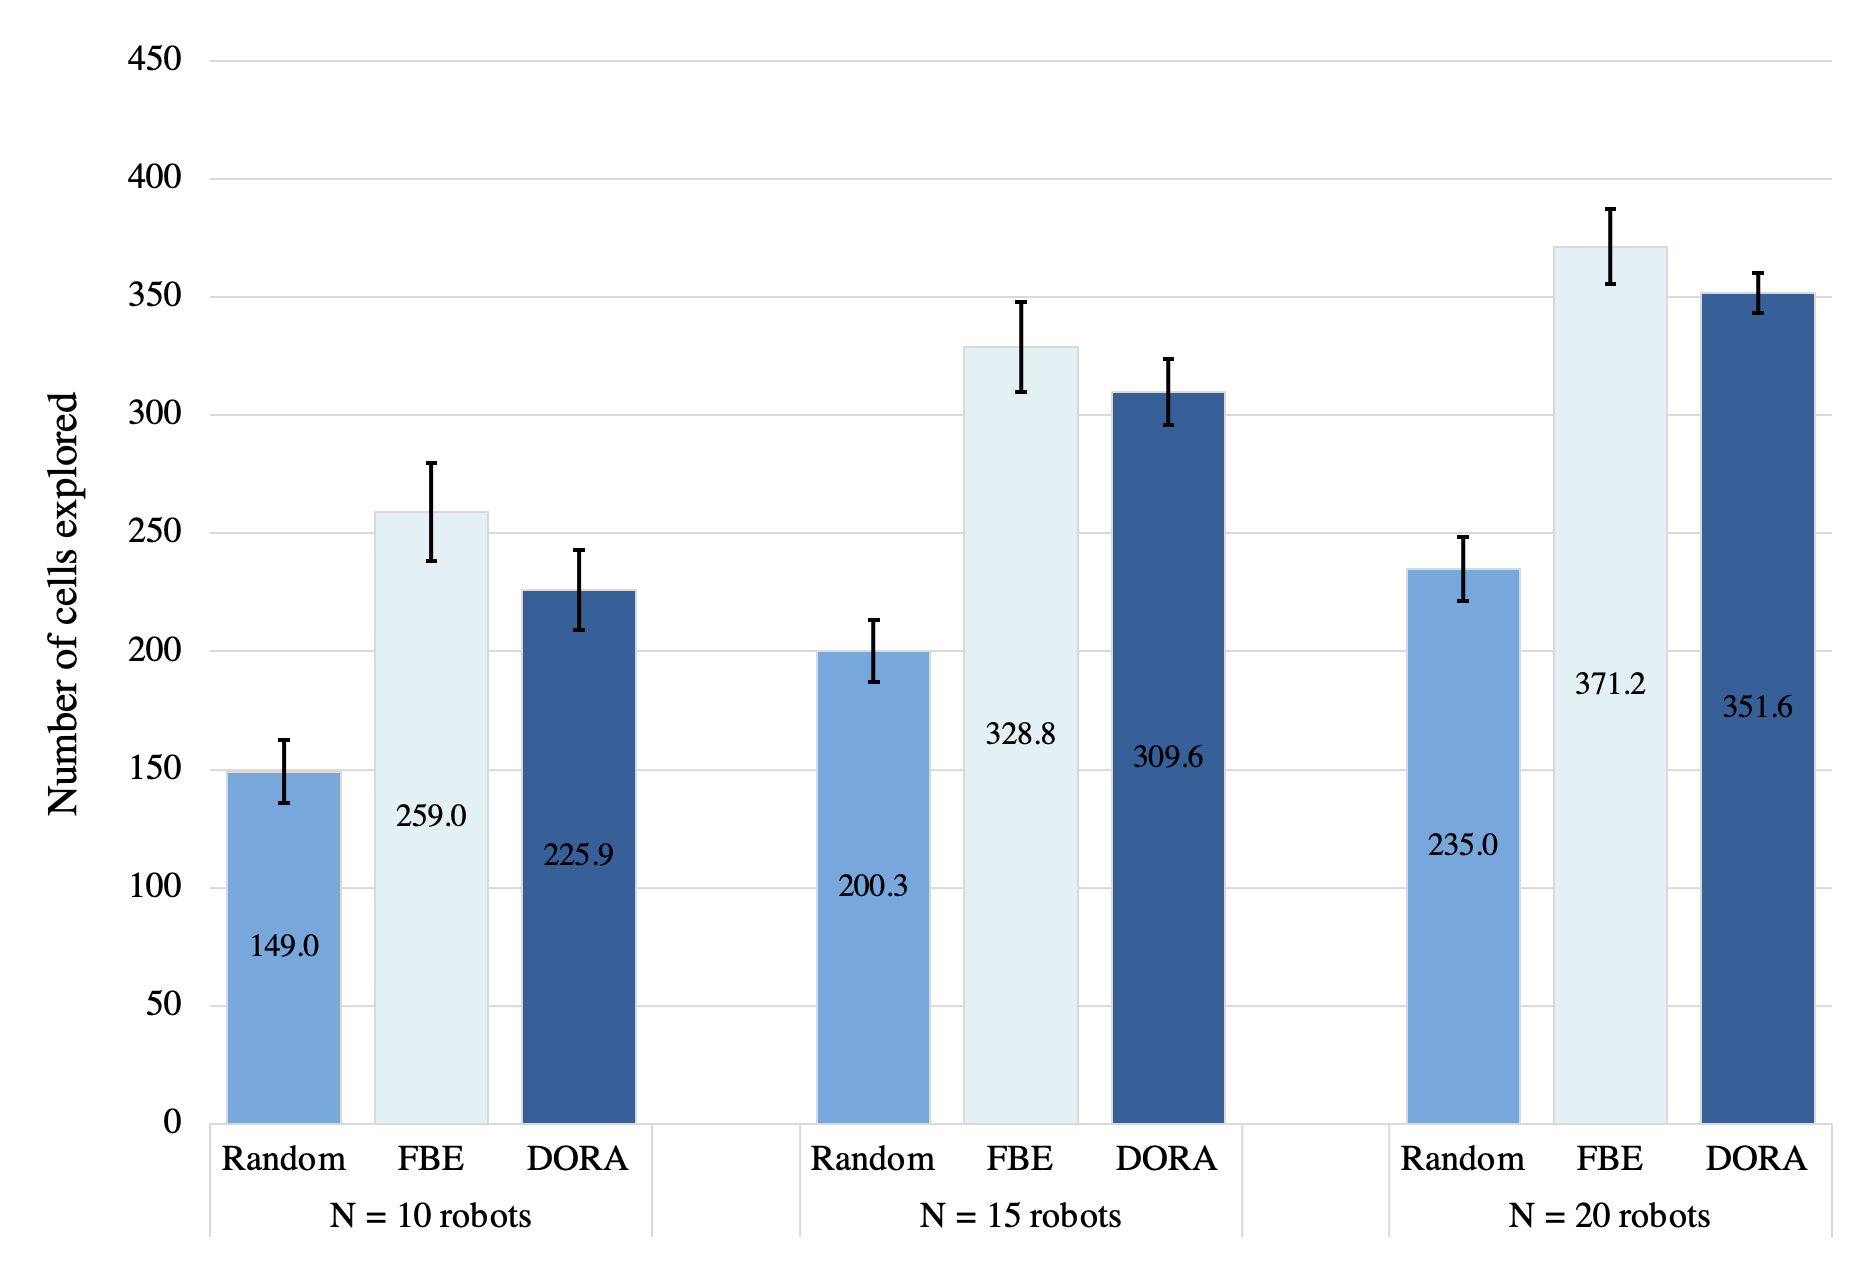
\includegraphics[width=1\columnwidth]{images/cell_explored.png}
    \caption{Performance comparison of DORA-Explorer, FBE and random walk for number of explored cells at the end of the simulation.}
    \label{results:exploration}
\end{figure}

\begin{figure}[]
    \centering
    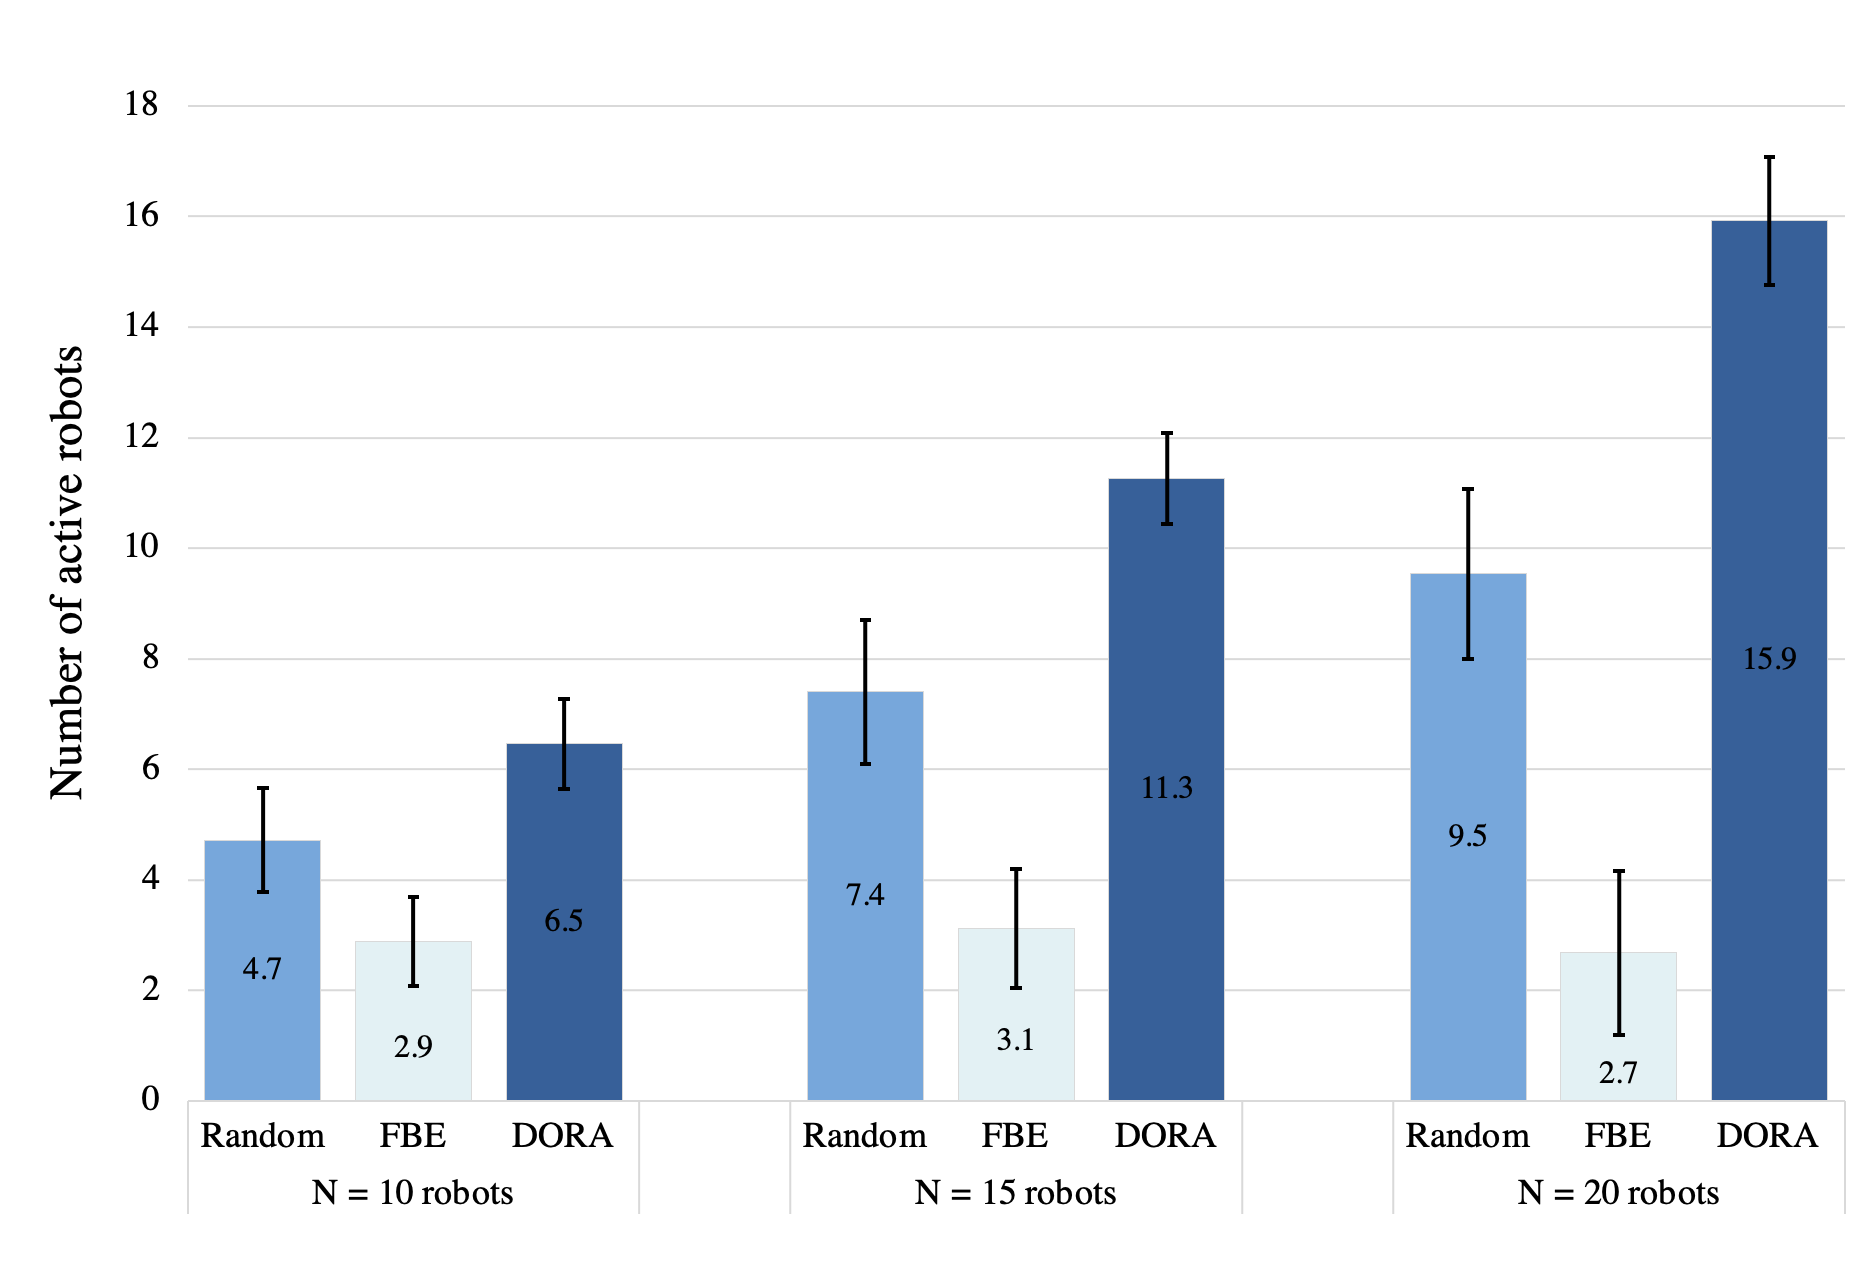
\includegraphics[width=1\columnwidth]{images/active_robot.png}
    \caption{Performance comparison of DORA-Explorer, FBE and random walk for number of active robots at the end of the simulation.}
    \label{results:active}
\end{figure}


Results from Fig. \ref{results:exploration} show that FBE
achieves slightly higher exploration coverage than DORA-Explorer, but this
gap in performance decreases as the number of robots increases. This
is an expected result, because DORA-Explorer's main goal is not to achieve
maximal coverage at all costs, unlike FBE. Both FBE and DORA-Explorer clearly
outperform the random walk algorithm. The other trend is that adding
more robots to the swarm results in a higher
number of cells being explored for all three algorithms after 300
steps. This shows that DORA-Explorer scales well to large number of robots, and even gains in performance when swarm size increases, which is in line
with the benefits associated with swarm algorithms. In terms of avoiding failures, DORA-Explorer unsurprisingly outperforms both
FBE and the random walk, as it is its main purpose. This is shown in
Fig. \ref{results:active}, where DORA-Explorer exhibits a higher level of active
robots at the end of the simulation runs, with this difference only increasing with larger
swarm sizes. For all values of N, there are few
survivors for FBE, and random walks perform only slightly better, while DORA-Explorer keeps most robots alive, achieving its objective.


Fig. \ref{results:belief} shows the DBMs obtained at the end of an
arbitrarily selected simulation where N = 20 for each algorithm.  In
other words, it represents which cells were explored by each algorithm
and the sensed radiation intensity associated with them for one specific run. 

\begin{figure}[h]
    \centering
    \begin{subfigure}{0.49\textwidth}
        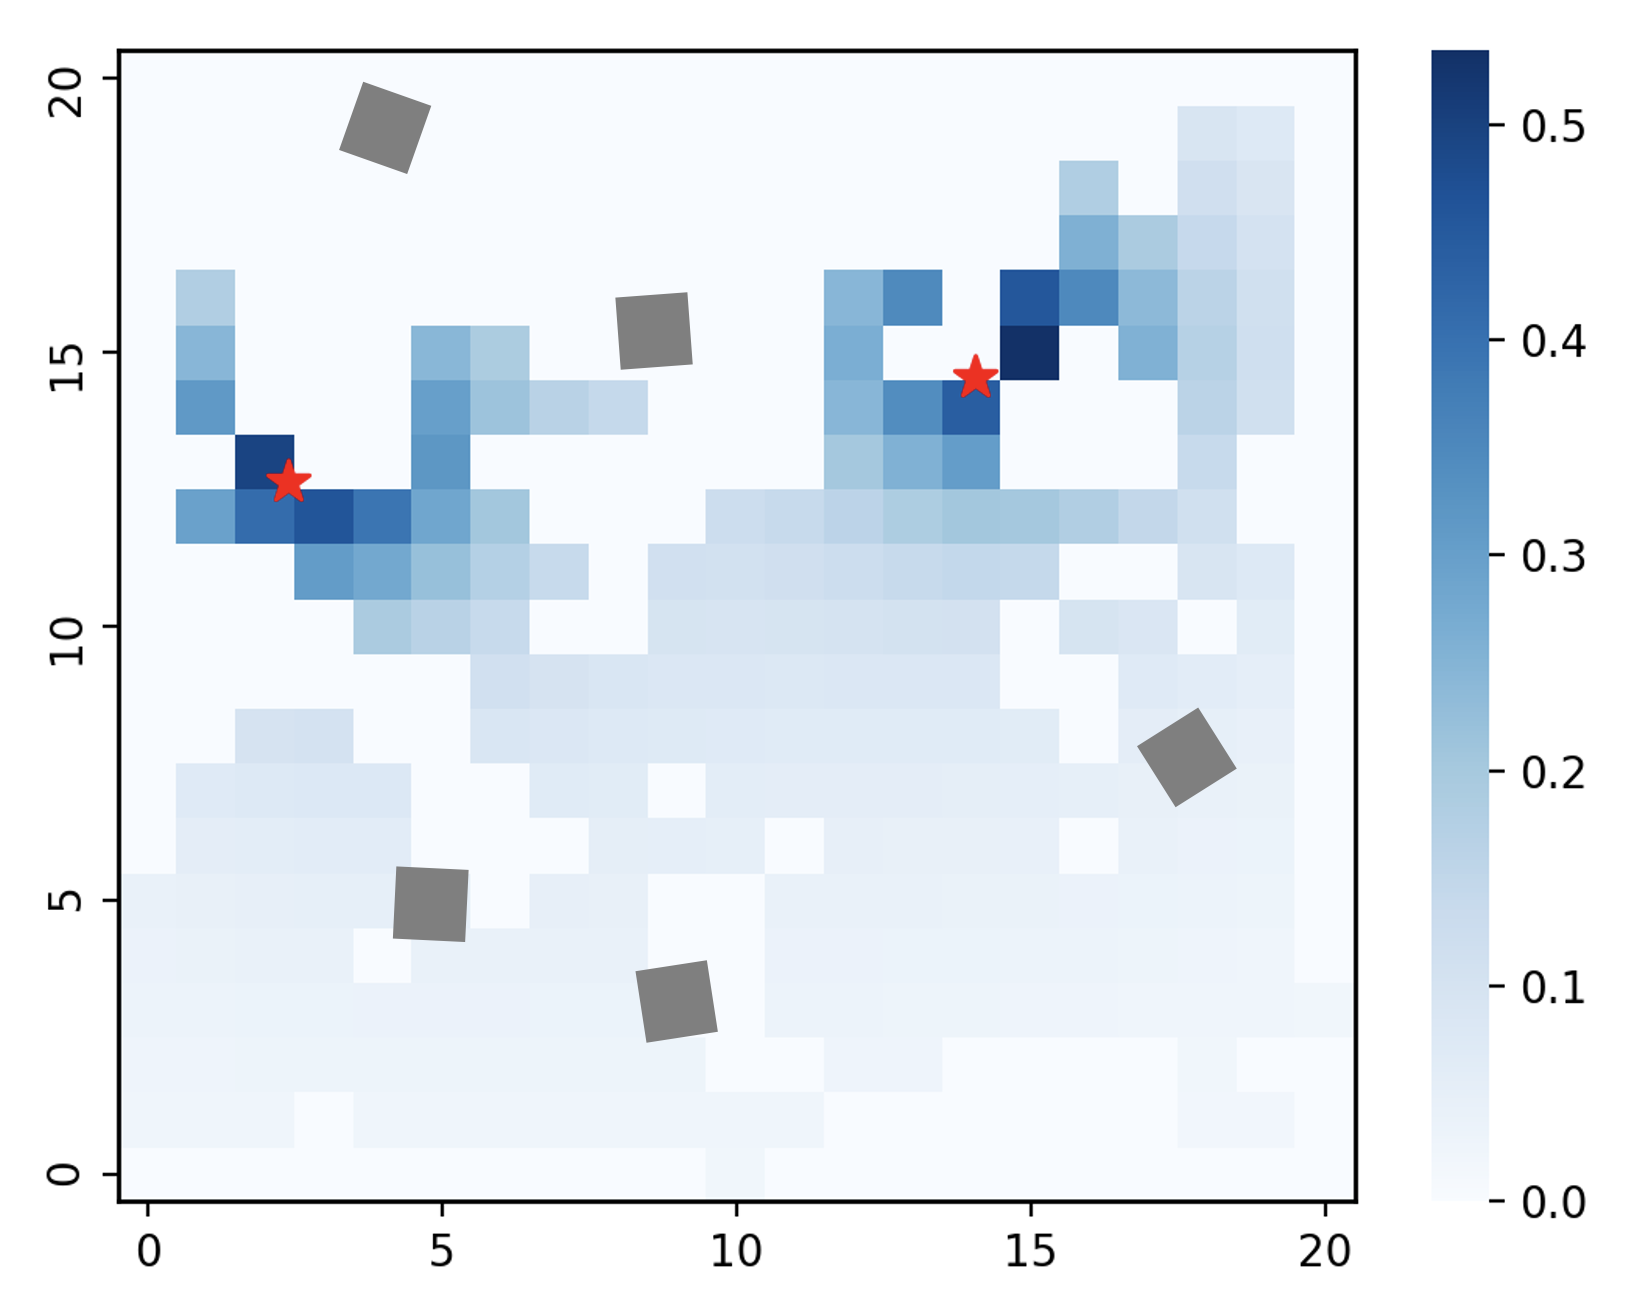
\includegraphics[width=\textwidth]{images/heatmap_random.png}
        \caption{Random walk}
        \label{results:beliefrandom}
    \end{subfigure}
    \begin{subfigure}{0.49\textwidth}
        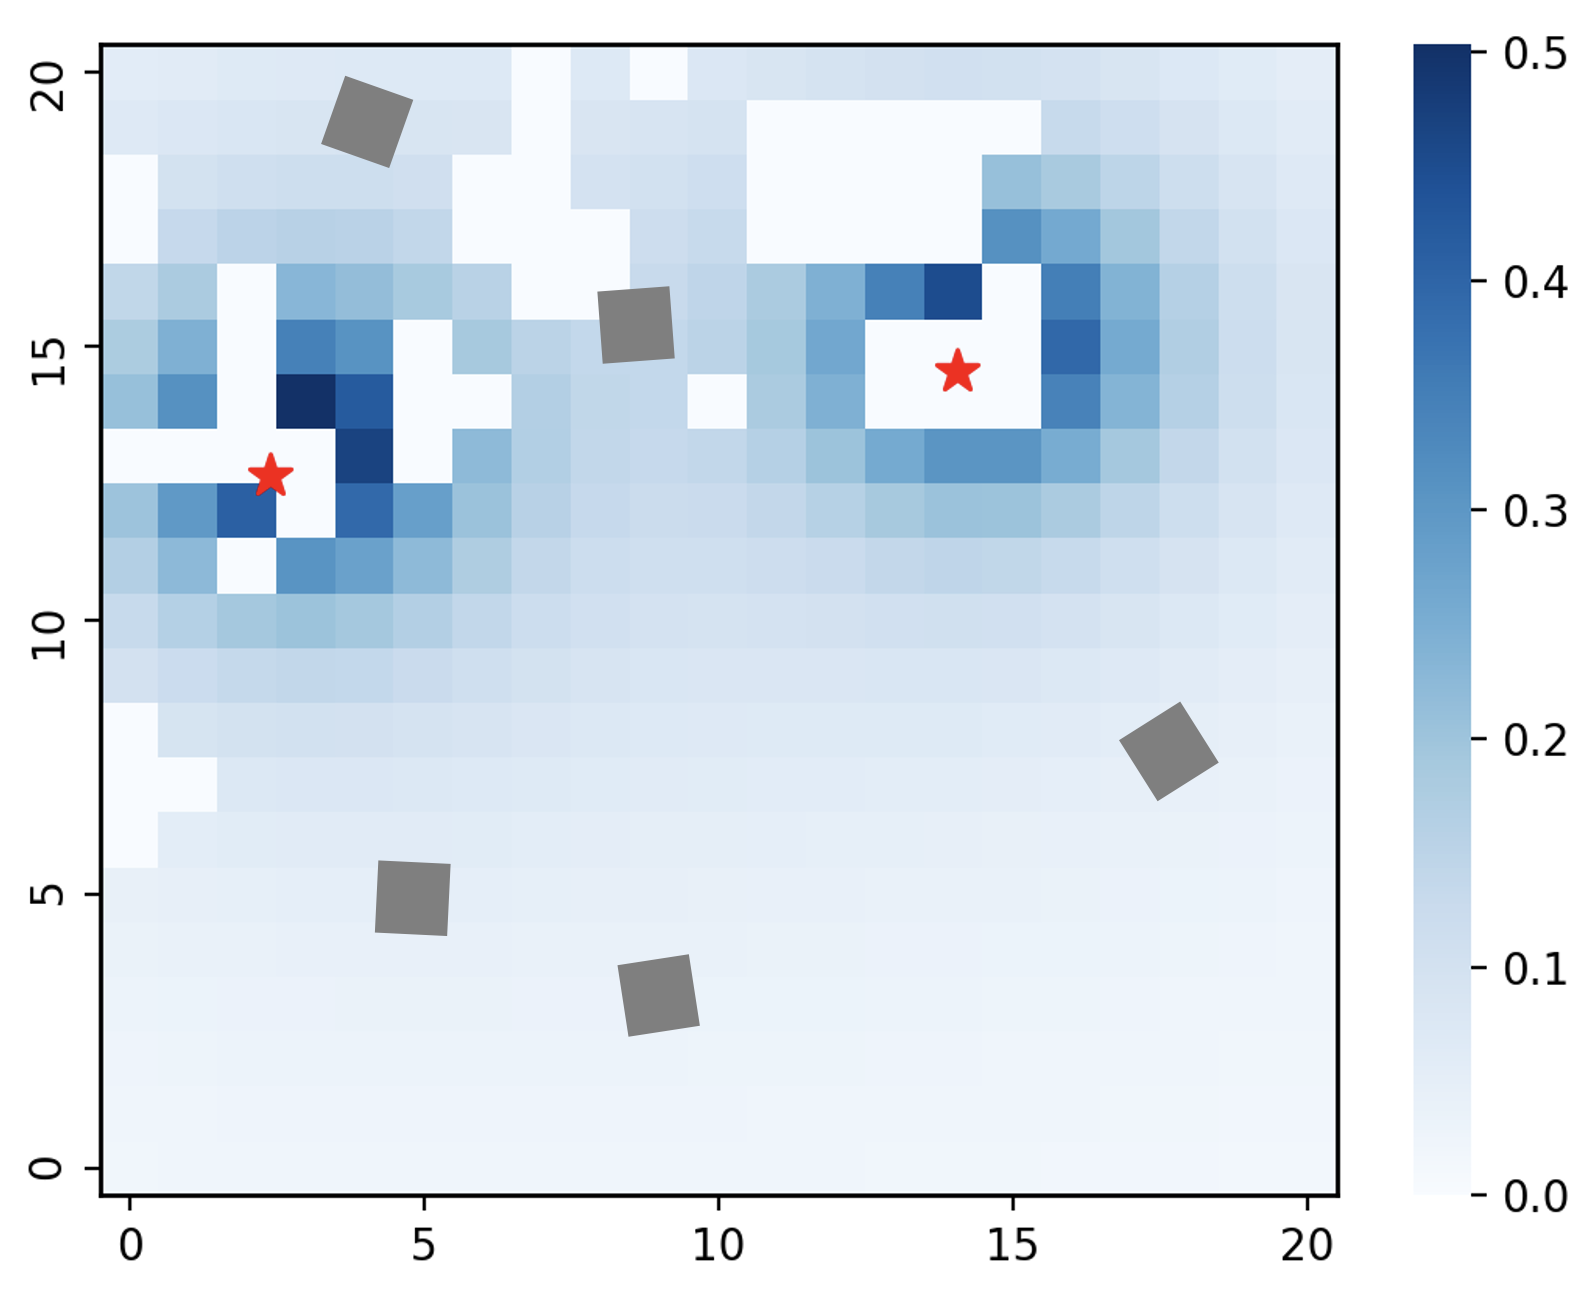
\includegraphics[width=\textwidth]{images/heatmap_frontier.png}
        \caption{FBE}
        \label{results:belieffrontier}
    \end{subfigure}
    \begin{subfigure}{0.49\textwidth}
        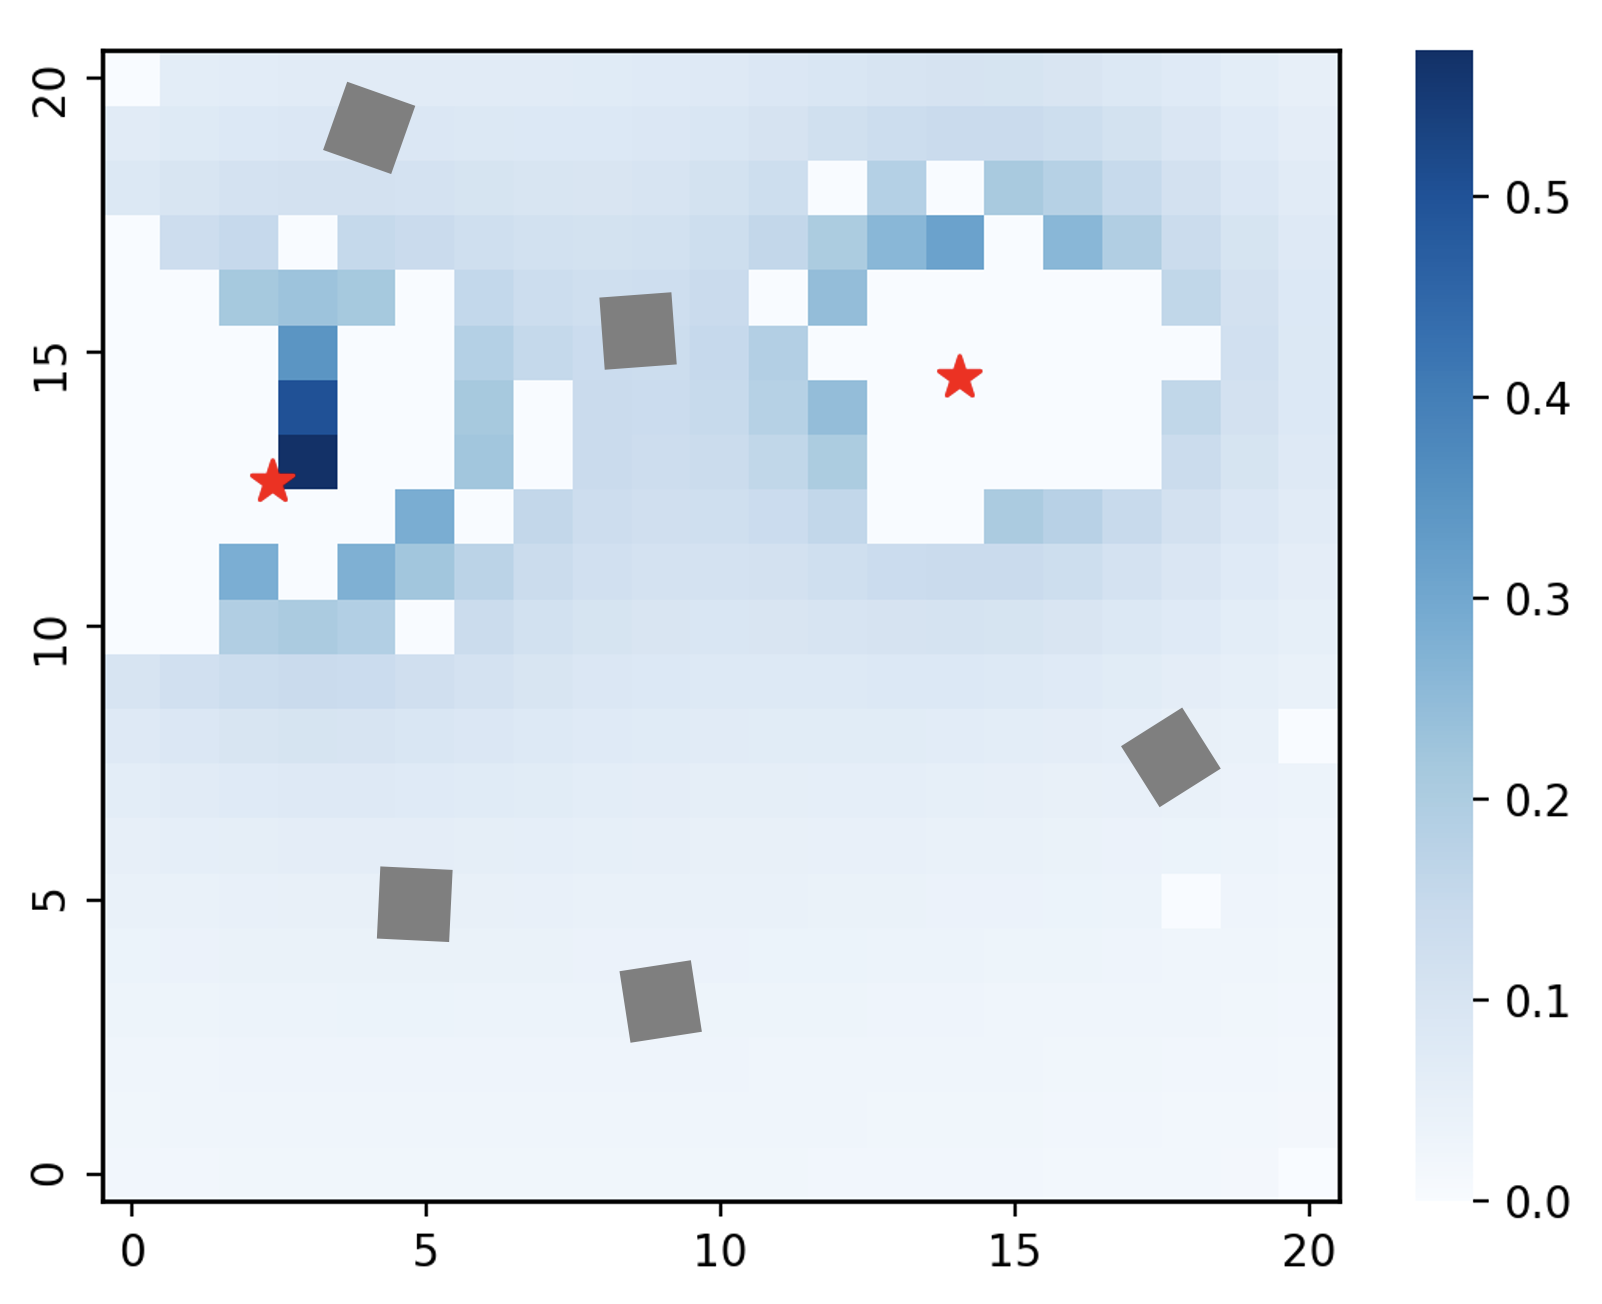
\includegraphics[width=\textwidth]{images/heatmap_dora.png}
        \caption{DORA-Explorer}
        \label{results:beliefdora}
    \end{subfigure}
    \caption{Radiation belief maps of the 20m x 20m environment for each exploration algorithm of one specific simulation. Blank cells are unvisited areas, red stars are the point radiation sources and grey squares are the randomly generated obstacles.}
    \label{results:belief}
\end{figure}

The random walk covered much fewer cells than DORA-Explorer and FBE, which both covered
roughly the same areas of the map, with the same sections remaining
unexplored. However, these areas remained unvisited for different
reasons. For FBE, the parts of the environment close to the radiation
sources remained uncovered because its agents failed when approaching
them. In contrast, DORA-Explorer did not explore these cells because it
\textit{avoided them}. Again, DORA-Explorer achieves very similar coverage than
FBE but does so with less robot failures. In this particular
simulation, DORA-Explorer finished with 18 active robots, random walk finished
with 7, and FBE with none. 


The results from Fig. \ref{results:communicationCosts} show the amount
of data transferred by individual agents at each time step by both
algorithms. We excluded the random walk algorithm from this figure as
it does not require any coordination or communication between its
agents. DORA-Explorer transmits more data than FBE, which was expected because
the former shares information through two DBMs, while the latter uses
only one. In section \ref{subsec:scalability}, we predicted that the
amount of data transmitted at each time step would only depend on the
size of the neighborhood used, and this is confirmed by
Fig. \ref{results:communicationCosts}, where it remains roughly
constant for different number of agents. The small increase in data
transmission with increasing number of robots can be attributed to
packet collision. 

\begin{figure}[h]
    \centering
    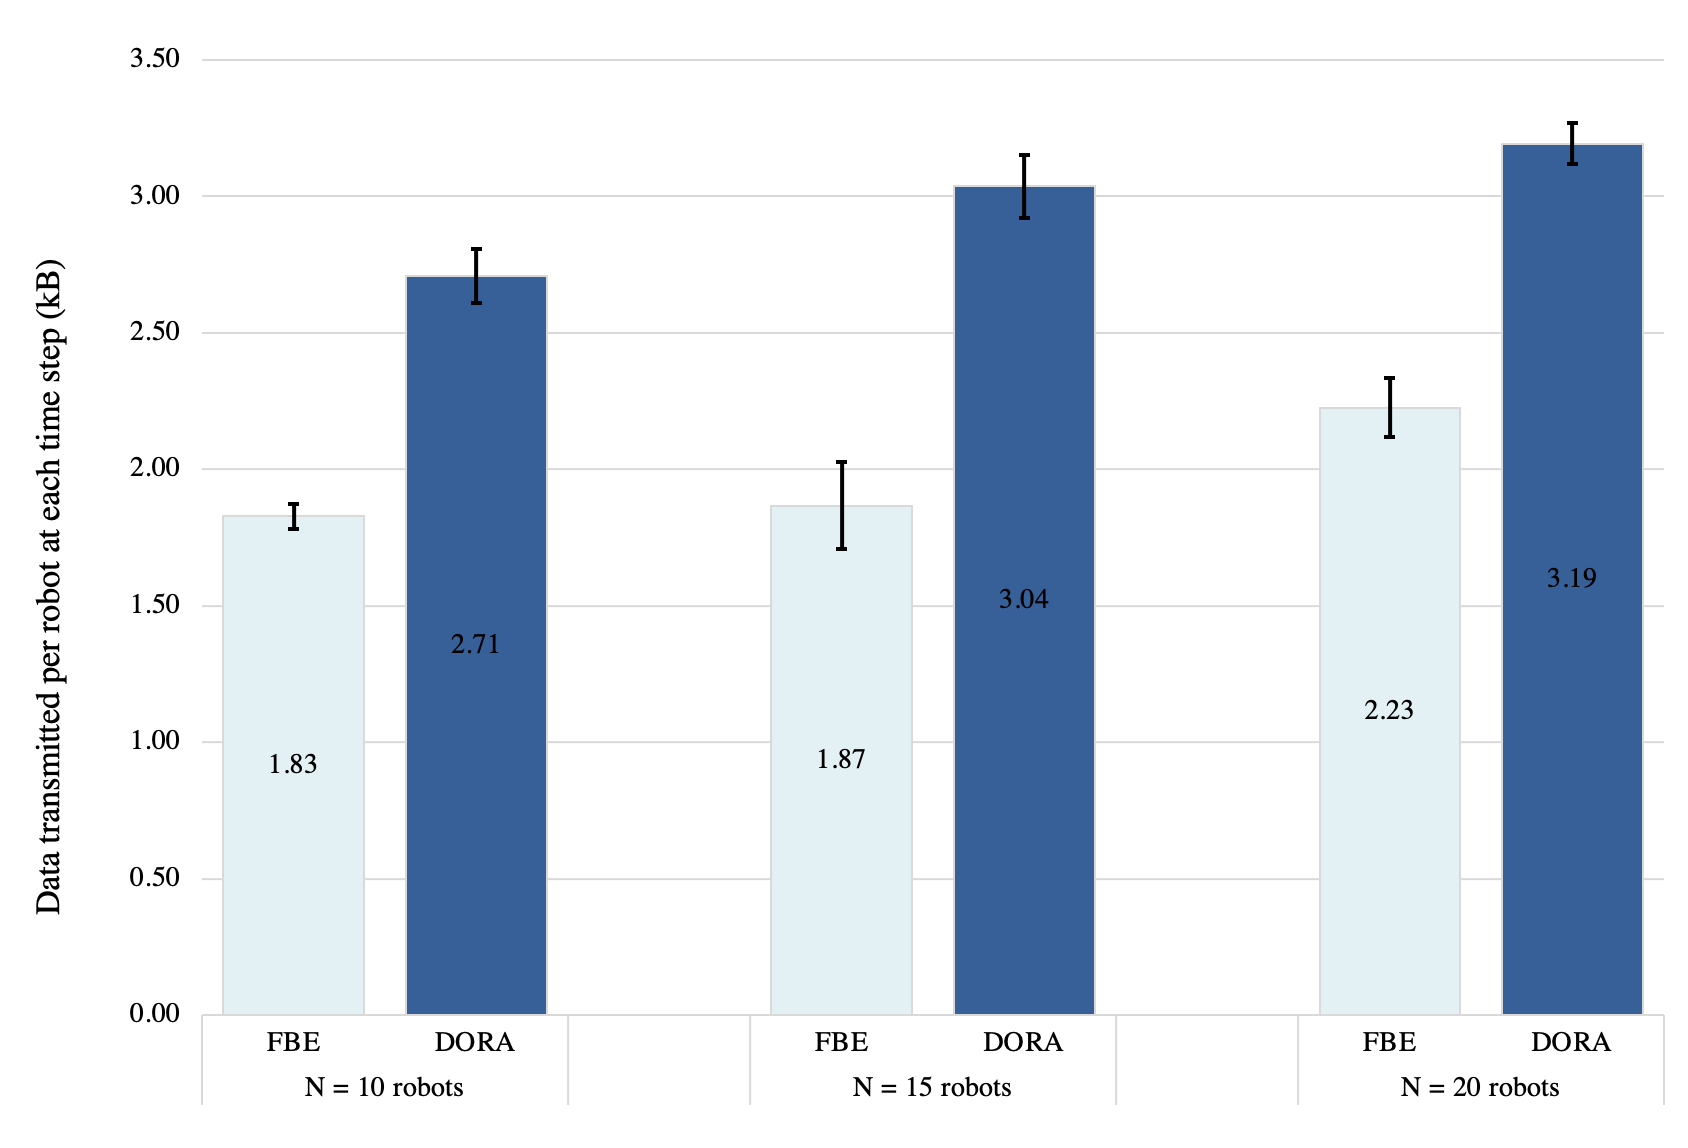
\includegraphics[width=1\columnwidth]{images/communication.png}
    \caption{Communication costs for DORA-Explorer and FBE}
    \label{results:communicationCosts}
\end{figure}

Results from Fig. \ref{results:parameters} show the performance of DORA-Explorer with varying ratios of risk gain $\alpha$ to exploration gain $\beta$. The experiments were carried with 10 robots. Results show that the number of remaining active robots at the end of the simulation only increases with a higher ratio. This is the expected behaviour as increasing the ratio corresponds to giving more importance to the risk avoidance gain from (\ref{eq:movement}). As for the number of cells explored, the relationship is not monotonic. In our experiments, a ratio $\alpha / \beta = 2$ provided the best result in terms of number of cells explored. For lower ratios, the robotic team is increasingly impacted by failures which in turns worsen the exploration performance. For higher ratios, the robot are too careful and don't explore as much the environment.

\begin{figure}[h]
    \centering
    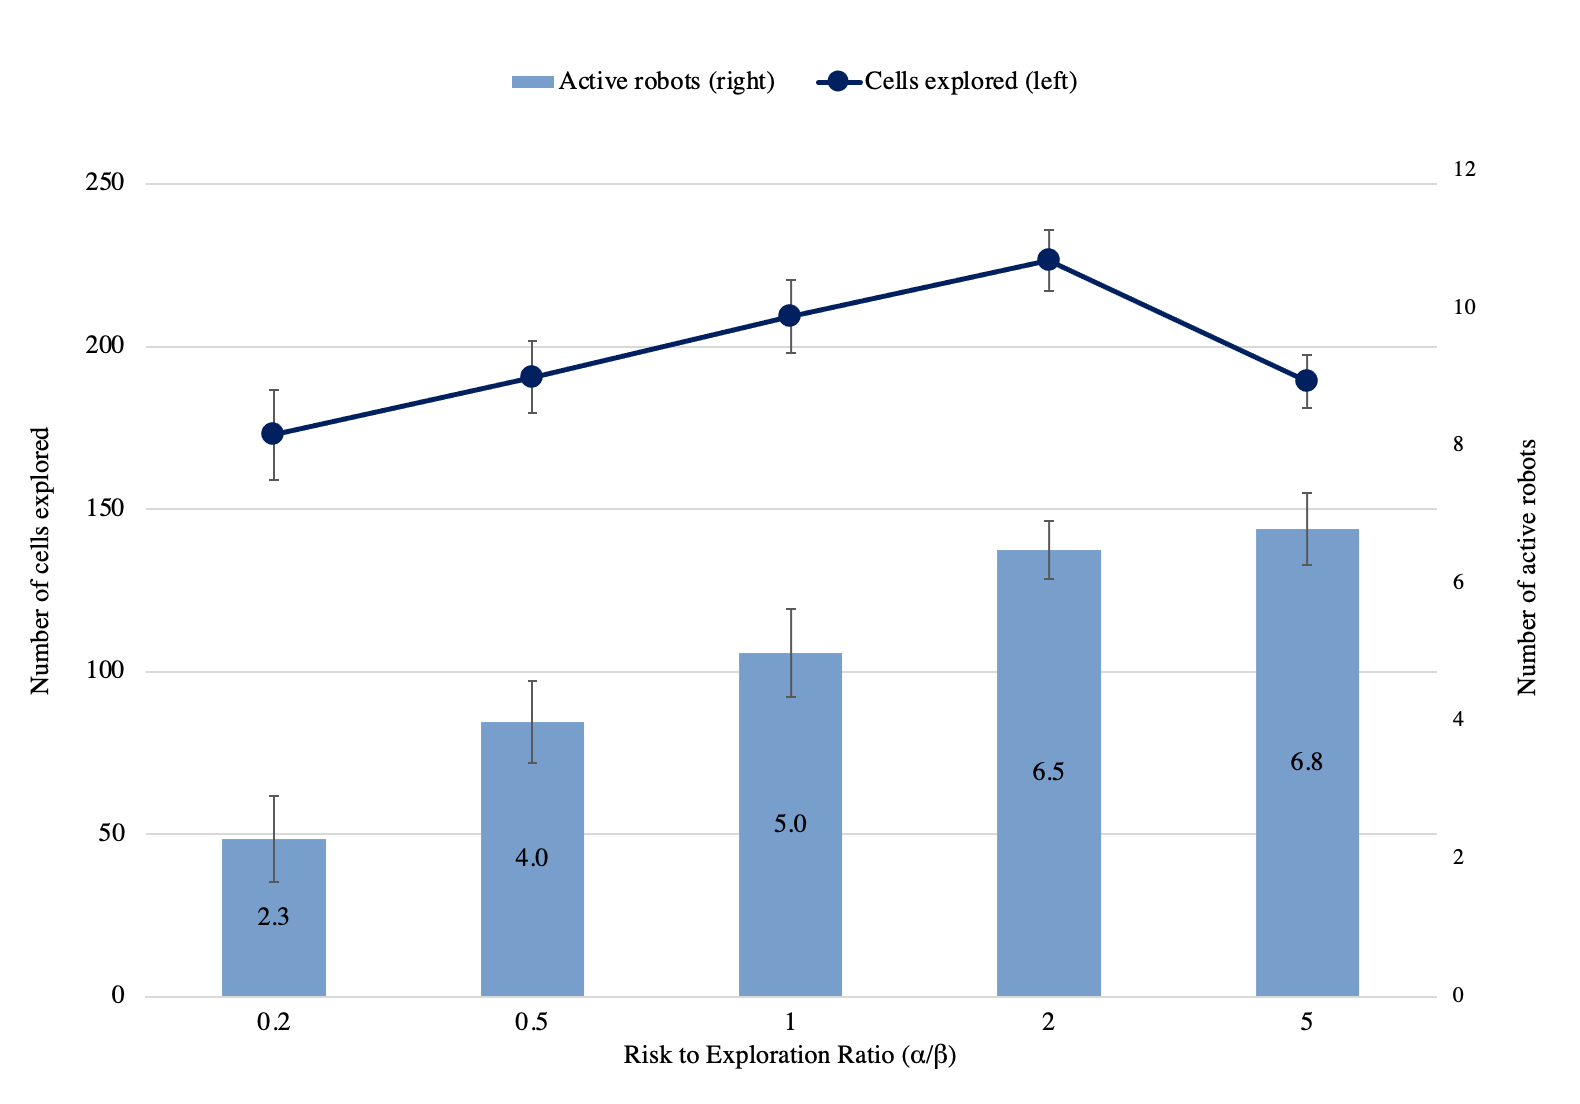
\includegraphics[width=1\columnwidth]{images/parameter.png}
    \caption{Performance of DORA-Explorer with varying ratios of $\alpha/\beta$}
    \label{results:parameters}
\end{figure}


\section{Physical experiments}
\subsection{Experimental setup}
In addition to the extensive simulations conducted in ARGoS, we tested
our system on a team of three physical KheperaIV robots in a 2x2m
environment containing 1 point radiation source. The environment is discretized as a 10x10 grid, meaning that each of
the 100 cells of the grid is 20x20cm large. Because the arena in
which we conducted the experiments was already limited in terms of
space we decided not to add obstacles.
Positioning of the
robots is done using an OptiTrack motion capture system. Radiation sensing is emulated
by an on board controller that reads the distance between the robot
and the radiation source to determine the current radiation
level. Failures are then triggered using equation \eqref{eq:failure}. If a robot fails, it stops moving and stops contributing to the exploration effort. The point
radiation source is located in a corner of the arena and the robots
are initially placed in the three remaining corners. We performed 5 runs over
200 steps of the DORA-Explorer algorithm. Each time step lasts 1s. Again, to assess DORA-Explorer's performance, we compare it to the results obtained by FBE and random
walk algorithms.

% \begin{figure}[h]
%     \centering
%     \captionsetup{belowskip=0pt}
%     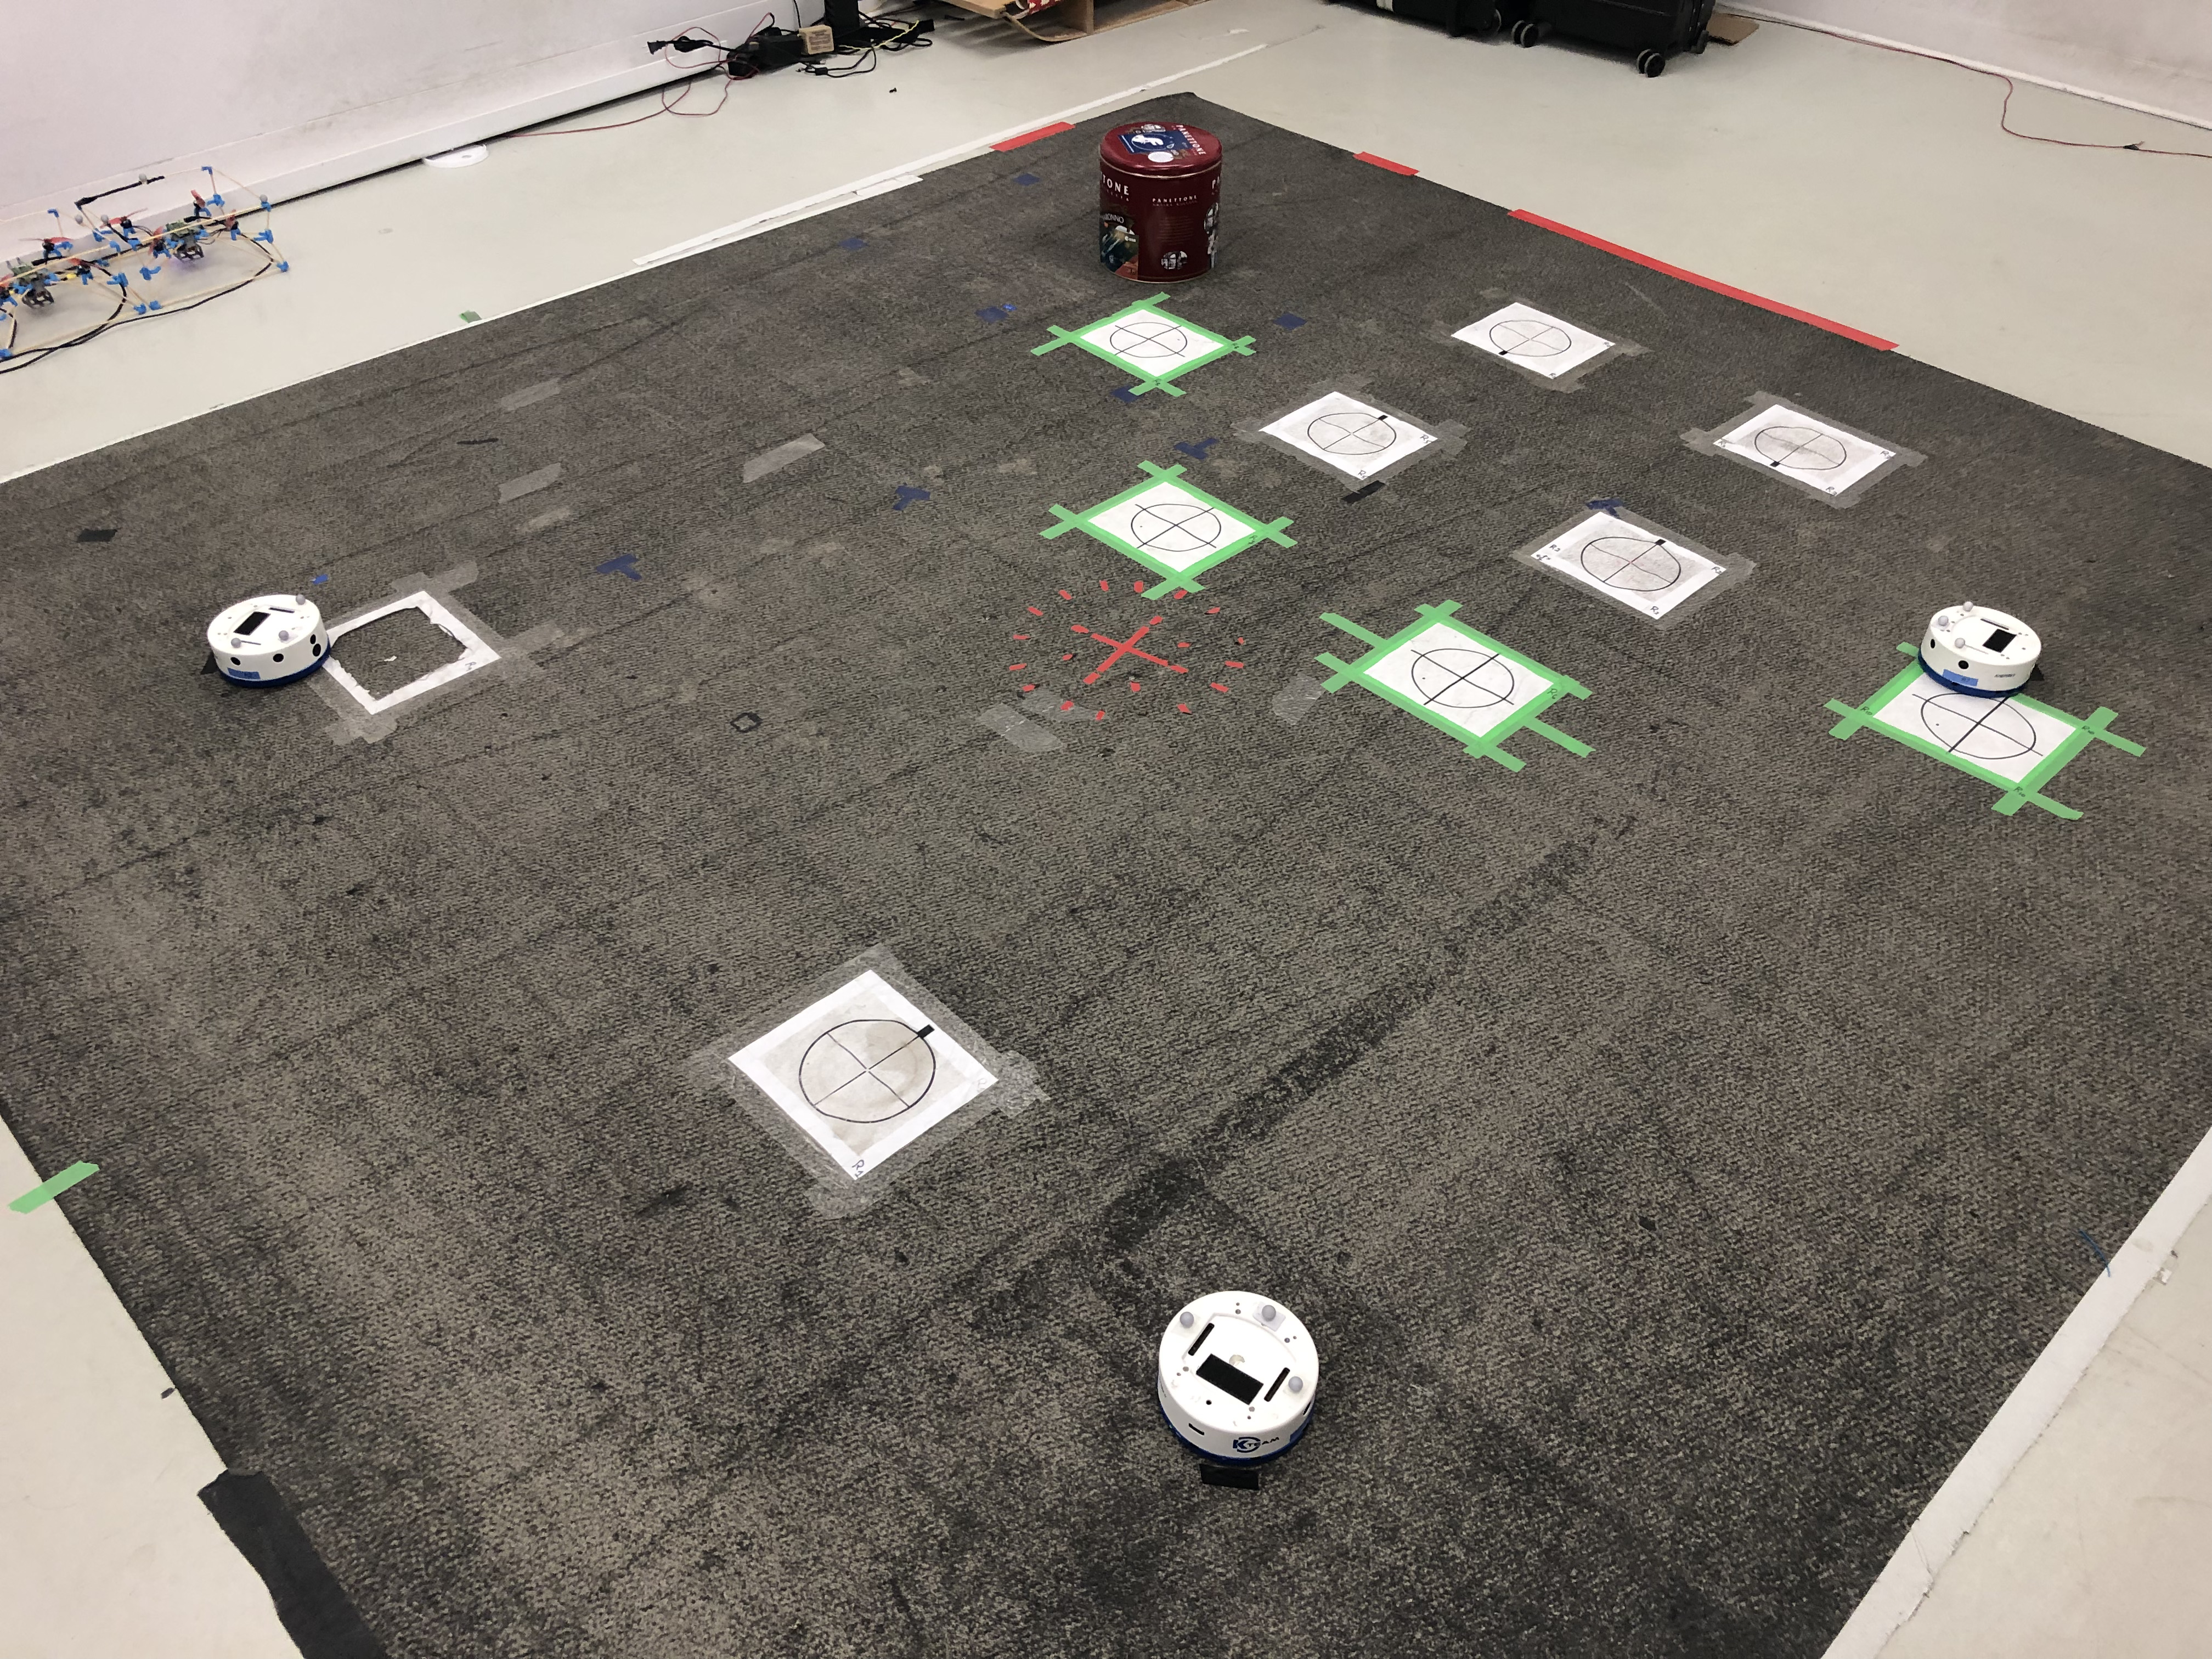
\includegraphics[width=0.65\columnwidth]{images/arena.jpeg}
%     \caption{Experiments on three physical KheperaIV robots. The red canister represents the point radiation source in the environment.}
%     \label{arena}
% \end{figure}


\subsection{Results}
The following results are an average of the 5 runs of each algorithm on physical robots.

\begin{figure}[H]
    \centering
    \captionsetup{belowskip=-5pt}
    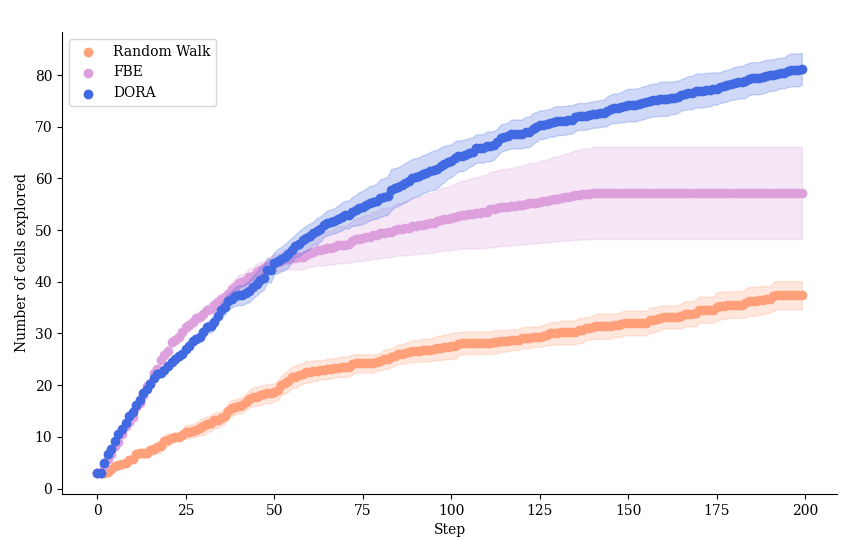
\includegraphics[width=0.82\columnwidth]{images/explored.png}
    \caption{Performance comparison of DORA-Explorer, FBE and random walk for number of explored cells over time on physical robots.}
    \label{results:cells_explored_physical}
\end{figure}

\begin{figure}[H]
    \centering
    \captionsetup{belowskip=-5pt}
    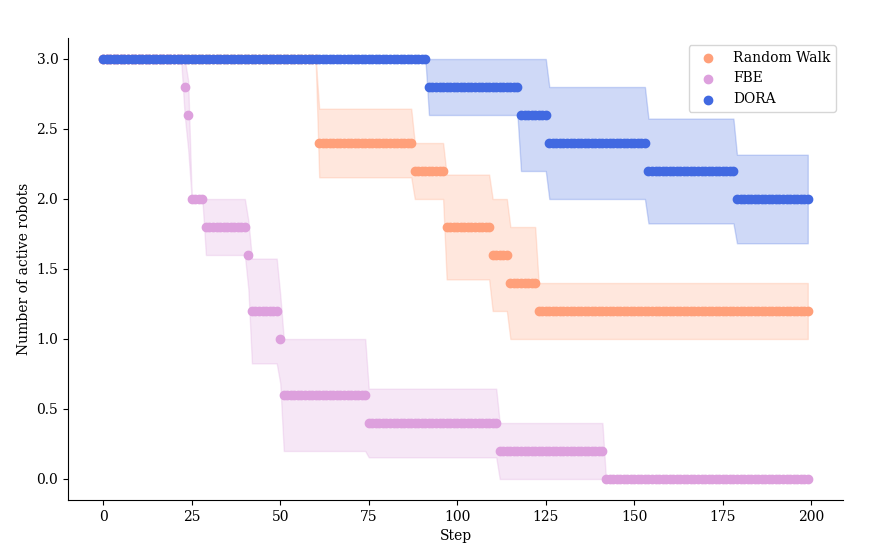
\includegraphics[width=0.82\columnwidth]{images/activerobots.png}
    \caption{Performance comparison of DORA-Explorer, FBE and random walk for number of active robots over time on physical robots.}
    \label{results:active_robots_physical}
\end{figure}

At the beginning of the exploration process, DORA-Explorer and FBE perform
similarly in terms of number of cells explored as shown in
Fig. \ref{results:cells_explored_physical}. The random walk
algorithm's exploration rate is considerably lower which can be
attributed to the fact that some of the cells of the environment are
visited multiple times: robots sometimes come back to positions that
they just had visited since their motion is determined randomly. As
time progresses, DORA-Explorer starts showing better exploration results than
FBE and at the end of the runs DORA-Explorer achieves a considerably better
coverage. Both FBE and DORA-Explorer clearly outperform the random walk
algorithm. In terms of robot failures, DORA-Explorer outperforms both FBE and the random
walk algorithm. This is shown in
Fig. \ref{results:active_robots_physical}, where DORA-Explorer exhibits a
higher level of active robots over time. When using FBE, all three
robots always fail before the end of the experiment. Random walk
shows a level of active robots that is in between DORA-Explorer and FBE. The results show that while DORA-Explorer and FBE initially have similar performances, as time progresses,
DORA-Explorer gets better when compared to FBE. The trend between DORA-Explorer and FBE in the physical experiments is inverted in comparison with the simulations because of the small environment into which the physical experiments were carried. Indeed, the likeliness of getting close of the radiation source was high, and as a result, without risk-awareness, the robots would fail very quickly. Because FBE
experiences a lot of failures, the failed robots stop exploring causing the exploration rate to decrease dramatically. In fact, FBE
always loses all its robots before the end of the experiments. In contrast,
DORA-Explorer keeps most of its robots active throughout the experiment and as a result the exploration rate remains high.


\section{Conclusion}
We presented DORA-Explorer, a novel lightweight risk-aware exploration
algorithm that minimizes the risk to which robots expose themselves in
order to maximize the amount of ground they will be able to cover. We expected that our exploration algorithm, which
leverages DBMs, would greatly outperform non-coordinated solutions,
and this has been the case. Indeed, it succeeded in reducing
considerably the likeliness of robot failures while keeping similar
ground coverage performance compared to other solutions proposed in
the literature. DORA-Explorer also showed good scalability thanks to its low
communication costs and its decentralized nature. It also showed applicability to real world
scenarios through experiments with physical robots. 

Taking inspiration from obstacle avoidance algorithms for the purpose of risk-avoidance could be an interesting future direction. Other future works include allowing DORA-Explorer to become more
or less risk-avoiding depending on the changing needs of the
situation. For example, in a search-and-rescue scenario, an increasing
urgency to rescue victims could motivate the willingness to take more
risks as time progresses. Also, more experiments could be conducted by
testing DORA-Explorer on a larger team of physical robots exploring
larger outdoor environments. Further applications of DORA-Explorer could
include using the generated risk belief map to determine robots'
fitness to store data in distributed storage systems like SwarmMesh
\cite{majcherczykSwarmmesh2020}, with robots assigned to tasks in
dangerous regions being discouraged from storing sensitive
information. Finally, in this work we considered that risk could be sensed by an on-board sensor. However,
in some scenarios, the risk cannot be directly perceived by any
sensors. In these cases, the belief map could instead be constructed using the
previous failures of the agents by assigning risk to areas only where
failures have been detected in the past.
             % Premier thème (Doctorat) ou "Détails de la Solution" (Maîtrise).
\Chapter{RISK-AWARE ROUTING IN ROBOT SWARMS}\label{sec:Theme2}
\noindent\fbox{%
    \parbox{\textwidth}{%
        \textbf{Preface:} In this chapter, the paper \textit{RASS: Risk-Aware Swarm Storage} \cite{arseneault2022rass}, to which I contributed as second author in the course of my master's degree is presented. RASS has been heavily inspired by DORA-Explorer and similarly to the latter, brings risk awareness to a robot swarm algorithm. Specifically, RASS makes the following contribution to the field of swarm robotics: A fully decentralized storing and routing algorithm where the decisions made are based solely on local interactions. The absence of central coordination makes it well suited for robot swarm applications where scalability is at the core of the problem.

        The figures presented in the chapter are taken from the article \cite{arseneault2022rass} with permission from the authors. 
        \\\\
        \textbf{Full Citation:} S Arseneault, D Vielfaure, G Beltrame. "RASS: Risk-Aware Swarm Storage". 2022.  International Conference on Autonomous Agents and Multiagent Systems (AAMAS).
    }%
}\\

\section{Introduction}
The exploration of unknown environments has proven to be more effective using teams of robots instead of a single robotic unit \cite{burgard2005coordinated}. Search and rescue scenarios \cite{kantor2003search} or nuclear inspection and cleanup \cite{schwagerMultirobotControlPolicy2017}, where speed is of the essence, are therefore well suited for multi-robot applications. However, data storage remains a challenge for such systems as the amount of collected information only increases with the number of robots. The unreliable connectivity that these systems typically suffer from \cite{amigoni2017multirobot} inhibits sending collected data items directly to external storage. Robots often need to store locally the data items until a path towards permanent storage becomes available. Additionally, because robots usually have a limited communication range, the data items collected during the mission may need to be routed through multiple robots before reaching the external storage infrastructure. The multi-robot system becomes a temporary storage infrastructure and deciding where to store and send the data items become essential. Routing the data items through the shortest path towards the base station may seem natural, however, because the environment into which the mission is carried is usually uncontrolled, environmental hazards can compromise some of the nodes of the system. For example, routing information through a robot located near a radiation source might cause data corruptions. Avoiding such nodes of the system can effectively increase the reliability of the system; thus risk should be considered when storing and routing data items. We propose a fully decentralized Risk-Aware Swarm Storage (RASS) system that actively routes data items towards a base station while avoiding dangerous nodes of the system. The algorithm relies solely on local interaction to determine which nodes are the fittest for storing information and works in both static and dynamic topologies.


\section{System model}
We consider a multi-robot system exploring an unknown environment in a fully decentralized fashion. The agents of the system, denoted as $a_i \in A$, are assumed to have limited storage capacities and communication capabilities. While exploring the environment, robots keep acquiring new data and try to convey the information to a base station for permanent storage. Because of their limited communication range $R$, robots may not be able to directly send data items to the base station. They might instead need to route the information through multiple robots before reaching the base station. Finally, point radiation sources $S$ with intensities $I_j\sim\mathcal{U}(0, 1)$ are randomly distributed in the environment.   

\subsection{Risk Modelling}
We assume the radiation sources to be the cause of data corruptions on nearby robots \cite{sharp1996radiation,messenger1986effects}. Figure \ref{risk_level_rass} shows an example of risk estimates held by robots based on their respective locations. The closer they are to the radiation sources, the higher the risk level will be. We assume the robots to be able to sense the radiation level associated with their current position using an on-board sensor.

\begin{figure}[htbp]
	\centering
    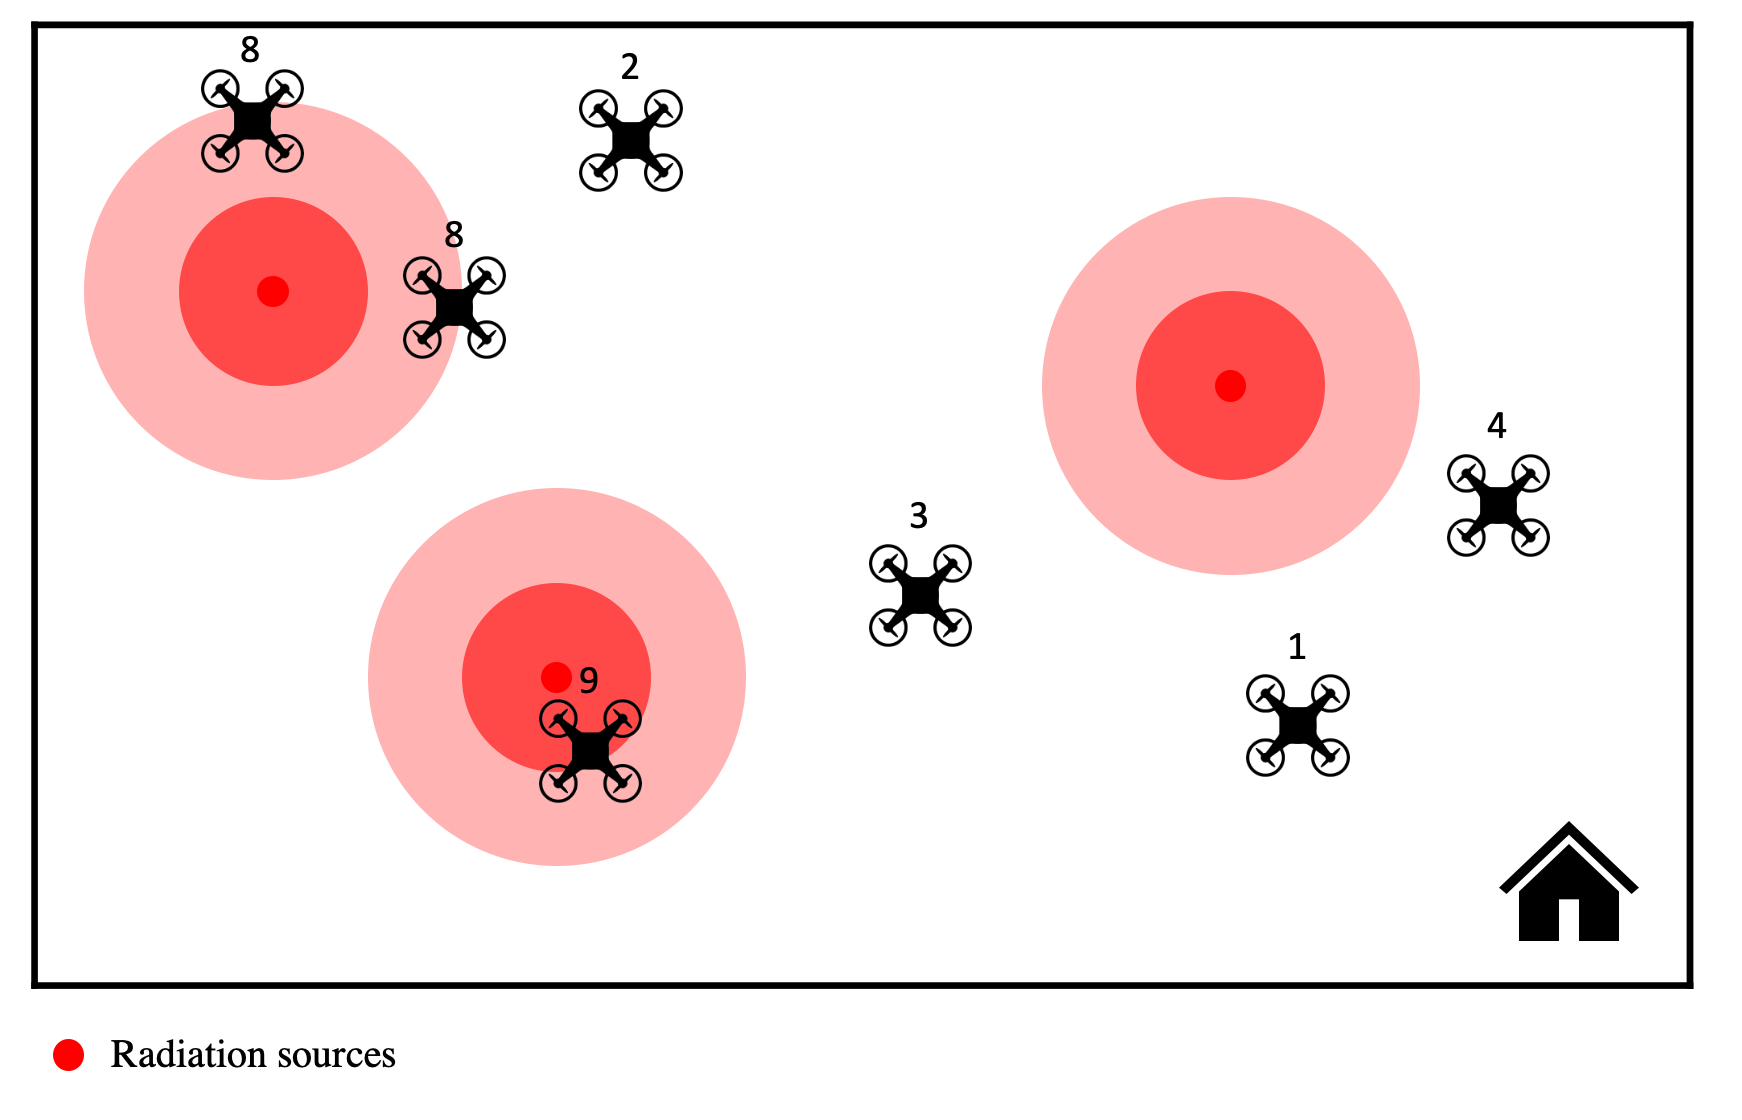
\includegraphics[width=0.75\columnwidth]{images/risk_rass.png}
    \caption{An example of risk levels (from 0 to 10) measured by robots}
    \label{risk_level_rass}
\end{figure}

The total radiation level perceived by a robot $a_i$ at position $\bm{x}_i \in E$ is given by:

\begin{equation}
    r(\bm{x}_i) = b + \sum_{\bm{s_j} \in S} \frac{I_{\bm{s_j}}}{1 + \lambda\rho(\bm{x}_i)^2}
    \label{eq:radiationRASS}
\end{equation}

The radiation level decays exponentially with the Euclidean distance $\rho(\bm{x}_i)$ between the position of the point radiation source $\bm{s}_j$ and the robot $\bm{x}_i$. $\lambda$ is used as a decay rate parameter and Gaussian measurement noise is added to the readings of the on-board sensor. 

We assume that the radiation sources affect the robots independently and therefore, the probability of data items to become corrupted is given by:

\begin{equation}
    \mathbb{P}(c_i = 1 | S) \sim \mathcal{B}(r(\bm{x}_i)) = 1 - \prod_{\bm{s_j} \in S} 1 - \mathbb{P}(c_i = 1 | \bm{s}_j)
    \label{eq:failureRASS}
\end{equation}


\subsection{Potential-Based Percolation}

RASS is built upon the assumption that nodes of the system exposed to higher levels of radiation should be used less for storing and routing data items. Indeed, because radiation is assumed to cause data corruptions, avoiding dangerous locations of the system should offer better reliability results and effectively reduce the number of lost data items. Additionally, to alleviate the memory usage of the robots of the system, percolating data items towards a base station for permanent storage should be encouraged. From this, and taking inspiration from \cite{majcherczykSwarmmesh2020}, we define a fitness policy that indicates how "fit" an agent is for storing data items. The fitness of an agent is given by:

\begin{equation}
        \phi_i =
        \left\{ 
        \begin{array}{ll}
            \frac{1}{\alpha h_i + \beta r({\bm{x}_i})} &\text{if } m_i > 0 \\
            0 &\text{otherwise}
        \end{array} \right.
        \label{equation:fitness}
\end{equation}

where $\alpha$ and $\beta$ are respectively the routing and risk control gains, $m_i$ is the available memory of agent $a_i$,  $r_i$ is the risk given by eq. \ref{eq:radiationRASS} and $h_i$ is the minimum hop count to the base station. An example of a minimum hop count gradient for a robot swarm is presented in figure \ref{hop_count_rass}. 

\begin{figure}[htbp]
	\centering
    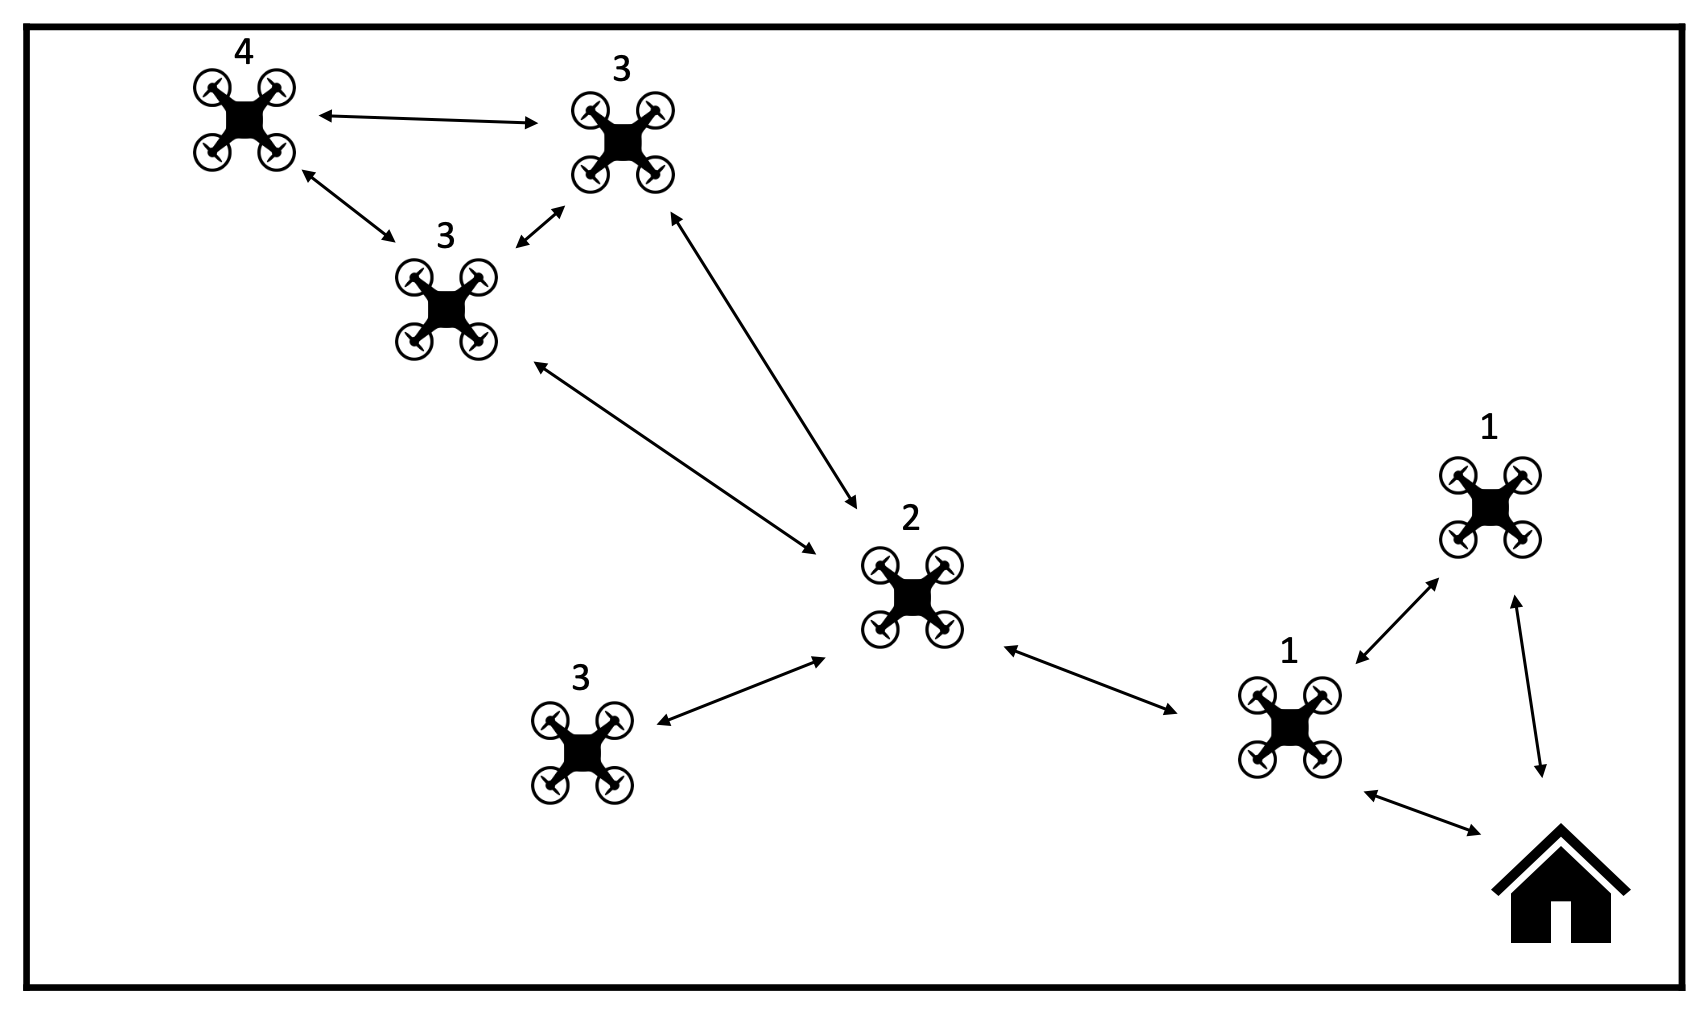
\includegraphics[width=0.75\columnwidth]{images/hop_count.png}
    \caption{An example of hop count distance to base station}
    \label{hop_count_rass}
\end{figure}

When a node becomes unfit to store data items, it will simply evict items to its fittest neighbour:

\begin{equation}
    T\phi_i < \max_{j \in \mathcal{N}} \phi_j
\end{equation}

$\mathcal{N}$ is the set of neighbours of agent $a_i$ and $T$ is a fitness threshold that ensures that data items are routed only when a neighbour is significantly better for storing them. 

Because of the hop count gain included in the fitness policy, data items will tend to passively percolate towards the base station. Indeed, for similar levels of risk, nodes located closer to the base station should have higher fitness. RASS' execution loop is summarized in algorithm~\ref{alg:rass}. Because of its fully decentralized nature, all the robots of the swarm execute the same code.

\begin{algorithm}[htbp]
\small
\SetAlgoLined
\DontPrintSemicolon
    \While{Running}{
        $get\_hop\_count()$\;
        $get\_risk\_measurement()$\;
        $update\_fitness()$\;
        \;
        \If{not $is\_fit()$ and $|\mathcal{N}| > 0$}{
            $evict\_data()$\;
        }
        \;
    }
 \caption{RASS Execution Loop}
 \label{alg:rass}
\end{algorithm}

\section{Simulations}

To assess the validity of our system, we tested RASS through simulations in the physics-based simulator ARGoS \cite{Pinciroli:SI2012}. The agents used
in the simulation are KheperaIV robots \cite{kteam2021kheperaiv} and RASS' implementation is done using the Buzz programming language from \cite{pinciroliBuzz2016}.

To thoroughly assess RASS' performance, four different robot topologies were studied:

\begin{itemize}
    \item Grid like pattern (static topology) as shown in figure \ref{argos:grid}
    \item Scale-free pattern (static topology) as shown in figure \ref{argos:scale-free}
    \item Lennard-Jones potential interactions (dynamic topology) as shown in figure \ref{argos:lennard-jones}
    \item Random search motions (dynamic topology) as shown in figure \ref{argos:random-walk}
\end{itemize}

\begin{figure}[htbp]
	\centering
    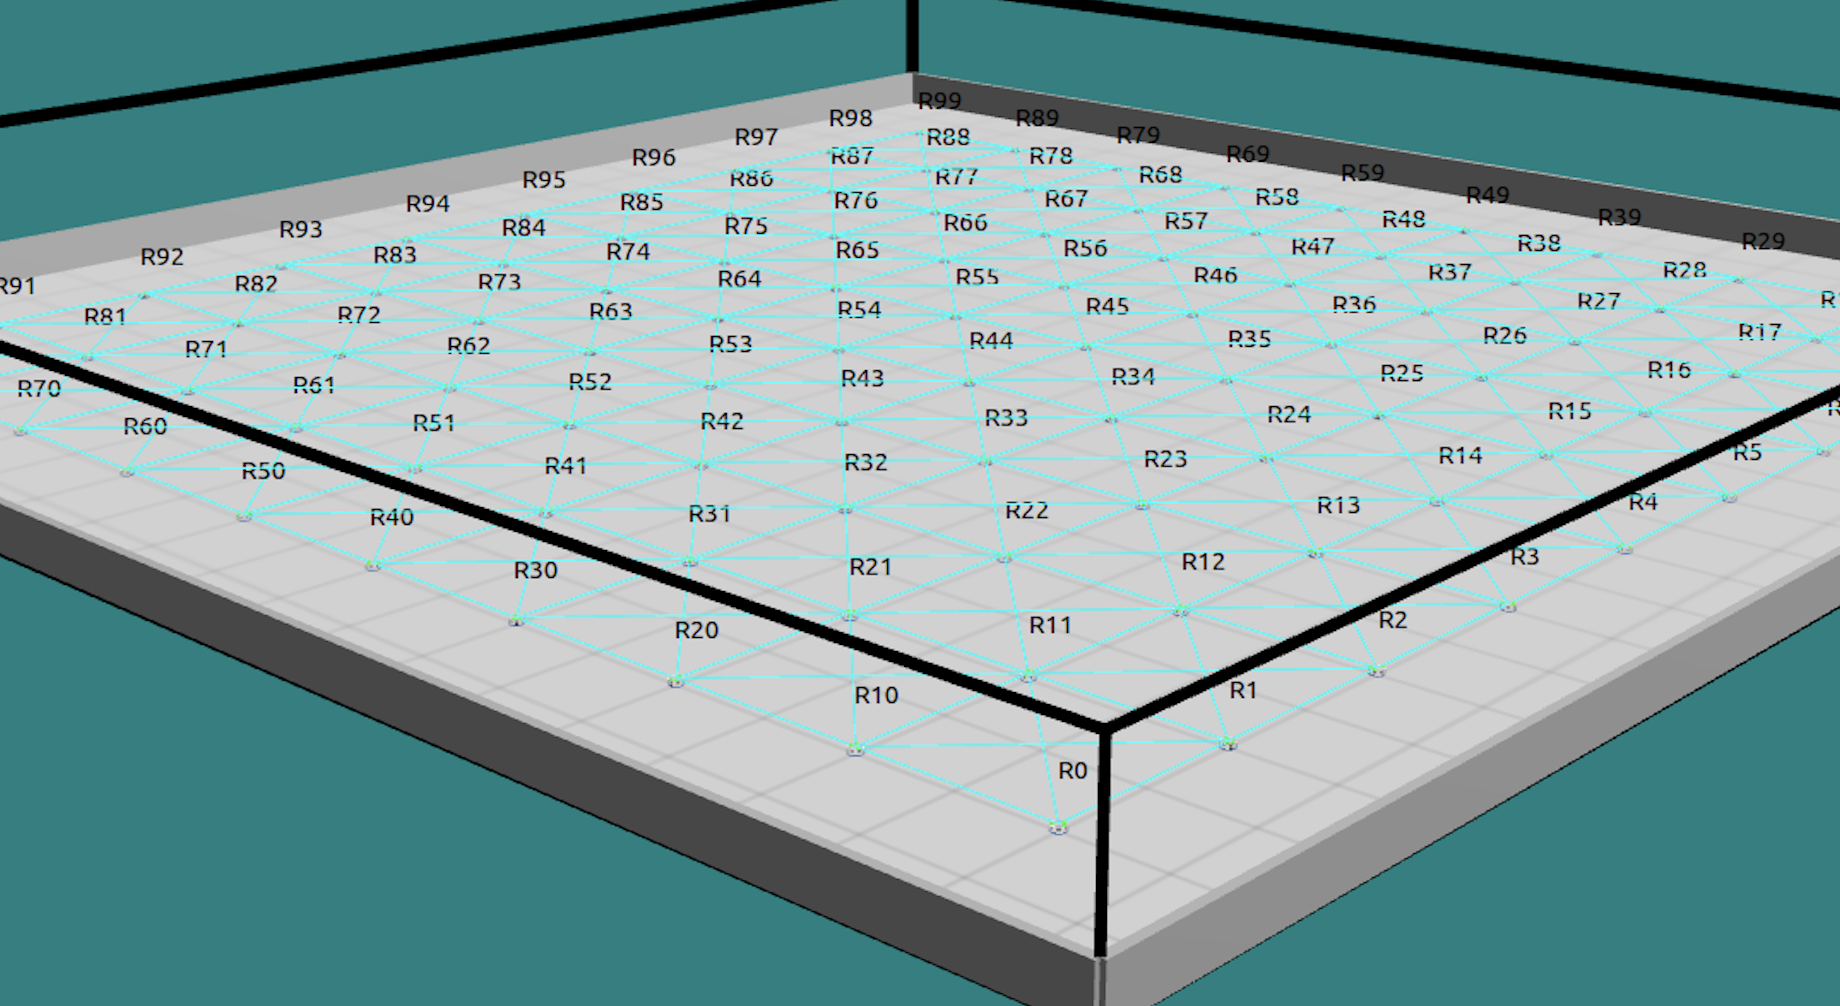
\includegraphics[width=\columnwidth]{images/argos_grid_link.png}
    \caption[Grid formation in ARGoS]{100 KheperaIV robots in 20m x 20m  ARGoS simulated environment distributed in a grid-like pattern.}
    \label{argos:grid}
\end{figure}

\begin{figure}[htbp]
	\centering
    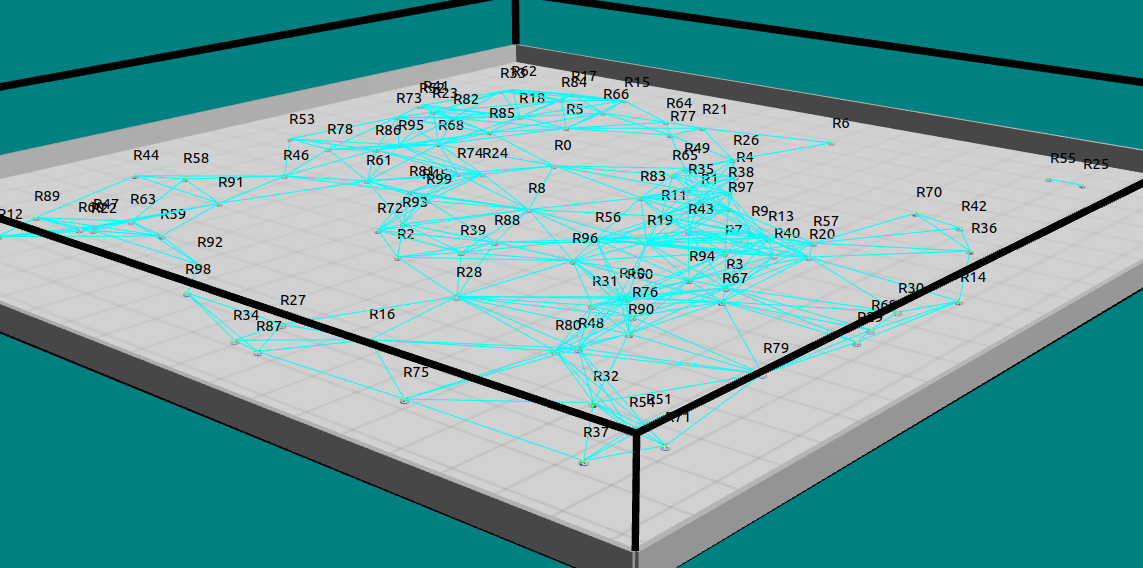
\includegraphics[width=\columnwidth]{images/argos_scale_free.png}
    \caption[Scale-free formation in ARGoS]{100 KheperaIV robots in 20m x 20m  ARGoS simulated environment distributed in a scale-free pattern.}
    \label{argos:scale-free}
\end{figure}

\begin{figure}[htbp]
	\centering
    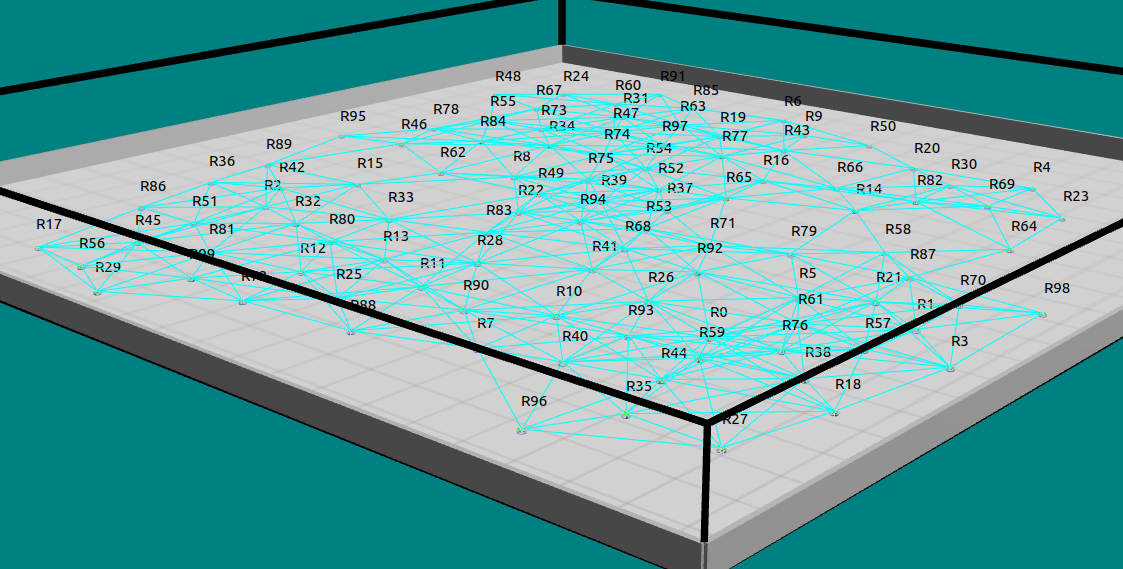
\includegraphics[width=\columnwidth]{images/argos_lennard.png}
    \caption[Lennard-Jones potential formation in ARGoS]{100 KheperaIV robots in 20m x 20m  ARGoS simulated environment in a dynamic topology obtained through Lennard-Jones potential interactions.}
    \label{argos:lennard-jones}
\end{figure}

\begin{figure}[H]
	\centering
    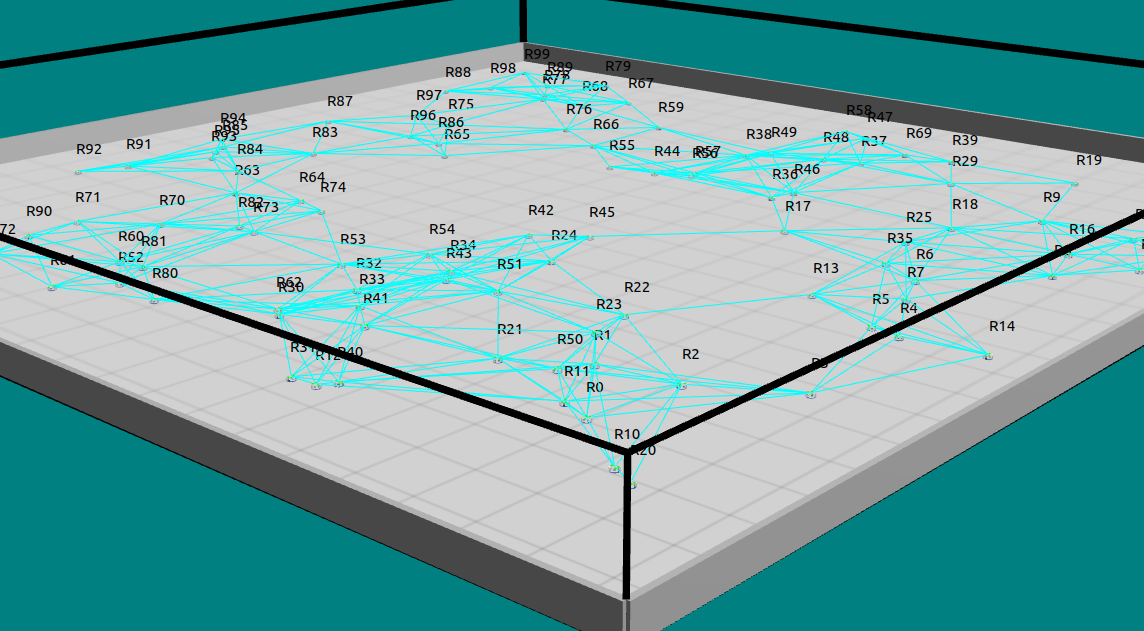
\includegraphics[width=\columnwidth]{images/argos_random.png}
    \caption[Random formation in ARGoS]{100 KheperaIV robots in 20m x 20m  ARGoS simulated environment in a dynamic topology obtained through random walk motions.}
    \label{argos:random-walk}
\end{figure}

We deploy N = 100 robots with a communication radius $R$ = 3 meters in a 20m x 20m environment containing a set of 3 randomly distributed radiation sources. The base station's storage capacity is assumed to be infinite and is located in one of the corners of the environment. To bring our simulations closer to real-world scenarios, we added bandwidth restrictions to the amount of data robots can possibly exchange. In our simulations, the maximal number of data items that could be exchanged between two neighbouring robots was 10 items every time step. Data items were generated at a fixed interval by all robots in the system. The storage capacity of robots was set to 50 data items. For our simulations, we used $\alpha = 10$ and $beta = 1$ for Eq. \ref{equation:fitness}. This choice was justified by the fact that the risk $r({x_i})$ was bounded by [0,1] while the hop-count value $h_i$ was not. In our simulations, $h_i$ was usually upper-bounded by 10. Therefore, choosing of value of $\alpha = 10$ gave the two parameters a similar importance when determining the fitness in Eq. \ref{equation:fitness}. Two benchmark algorithms were used to assess RASS' performance:

\begin{itemize}
    \item A routing algorithm based on hop count 
    \item The virtual stigmergy from \cite{pinciroliTuple2016}
\end{itemize}

The hop-count based algorithm enables comparison with a commonly used routing mechanism meant to yield fast transfer speeds. The virtual stigmergy was chosen to showcase the benefit of percolating data towards a base station.

The results obtained in the simulations for the different topologies are presented in Fig. \ref{results:staticTopology}, \ref{results:staticTopologyScale}, \ref{results:dynamicTopologyLennard} and \ref{results:dynamicTopologyRandom} as well as in table \ref{table:speed}. They show that RASS persistently outperforms the hop-count based algorithm and the virtual stigmergy in terms of reliability across all four topologies. Indeed, the percentage of retained data for RASS is usually between 80\% and 100\%, meaning that no more than 20\% of generated data items during the experiments are lost due to corruption. On the other hand, the hop-count based algorithm offers reliability results ranging from 50\% to 80\% and is therefore more affected by the radiation sources of the environment. Finally, the virtual stigmergy offers low reliability results as the storage capacity of the agents is quickly saturated and new data items cannot be stored any more. In terms of transfer speeds, results show that the fastest routing mechanism is the hop-count based algorithm. In average, RASS is 54.9\% slower than the hop-count based algorithm, in other words, it takes 54.9\% more steps for data items to reach the base station using RASS. This is not surprising as the hop-count based algorithm always takes the fastest route to the base station, without considering the risk associated with it. In opposition, RASS takes the route that optimizes both speed and safety. RASS offers better reliability results at the cost of slower transfer speeds.  

\begin{figure}[htbp]
    \centering
    \subfigure[]
        {
        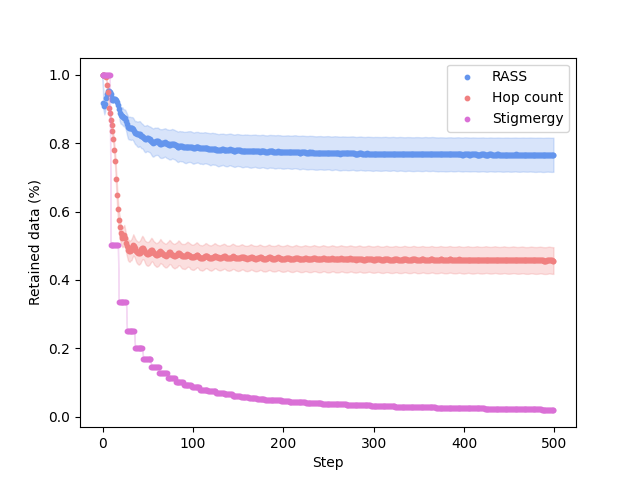
\includegraphics[width=0.75\textwidth]{images/grid_reliability.png}
        \label{results:grid_100_reliability}
        }
    \subfigure[]
        {
        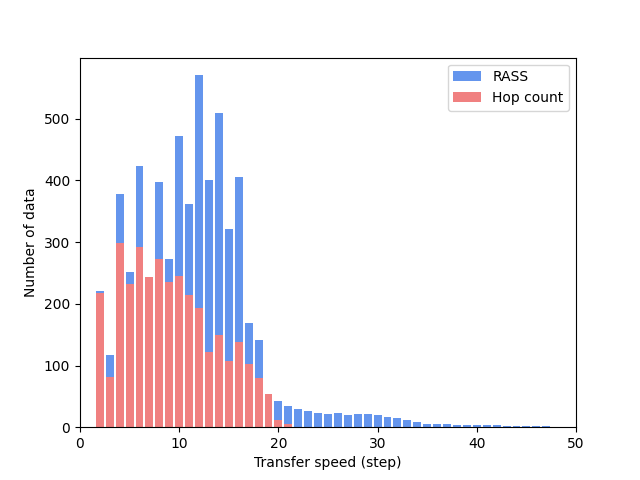
\includegraphics[width=0.75\textwidth]{images/grid_speed.png}
        \label{results:grid_100_speed}
        }
    \caption{(a) Reliability over time (b) Distribution of transfer speeds. Performance comparison of RASS, hop count and stigmergy in a static grid-like topology.}
    \label{results:staticTopology}
    \vspace{-2mm}
\end{figure}

\begin{figure}[htbp]
    \centering
    \subfigure[]
        {
        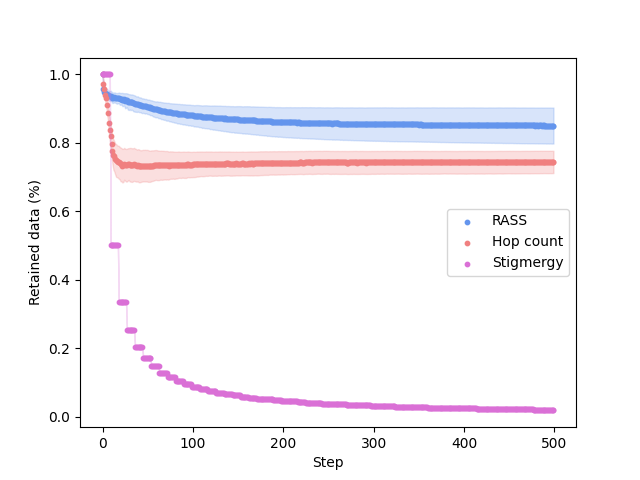
\includegraphics[width=0.75\textwidth]{images/scale_reliability.png}
        \label{results:scale_100_reliability}
        }
    \subfigure[]
        {
        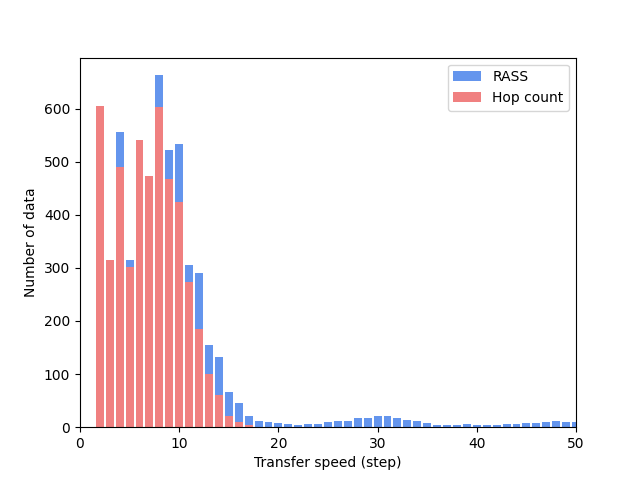
\includegraphics[width=0.75\textwidth]{images/scale_speed.png}
        \label{results:scale_100_speed}
        }
    \caption{(a) Reliability over time (b) Distribution of transfer speeds. Performance comparison of RASS, hop count and stigmergy in a static Scale Free topology.}
    \label{results:staticTopologyScale}
    \vspace{-2mm}
\end{figure}

\begin{figure}[htbp]
    \centering
    \subfigure[]
        {
        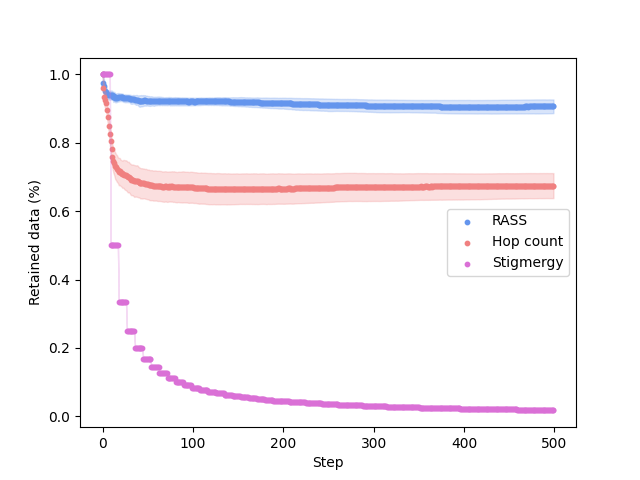
\includegraphics[width=0.75\textwidth]{images/lennard_reliability.png}
        \label{results:lennard_100_reliability}
        }
    \subfigure[]
        {
        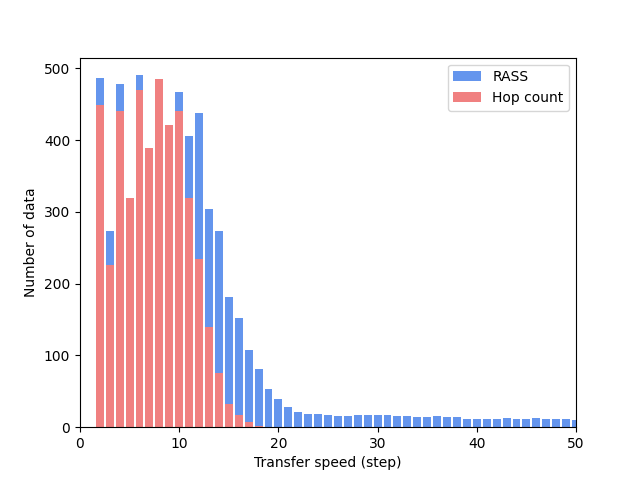
\includegraphics[width=0.75\textwidth]{images/lennard_speed.png}
        \label{results:lennard_100_speed}
        }
    \caption{(a) Reliability over time (b) Distribution of transfer speeds. Performance comparison of RASS, hop count and stigmergy in a dynamic Lennard-Jones topology.}
    \label{results:dynamicTopologyLennard}
    \vspace{-2mm}
\end{figure}

\begin{figure}[htbp]
    \centering
    \subfigure[]
        {
        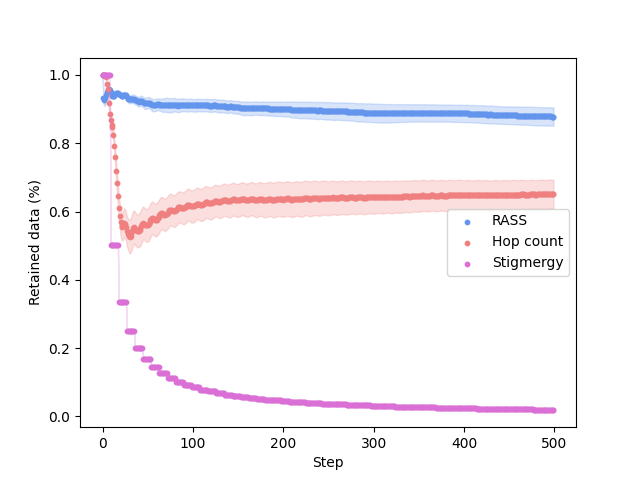
\includegraphics[width=0.75\textwidth]{images/random_reliability.png}
        \label{results:random_100_reliability}
        }
    \subfigure[]
        {
        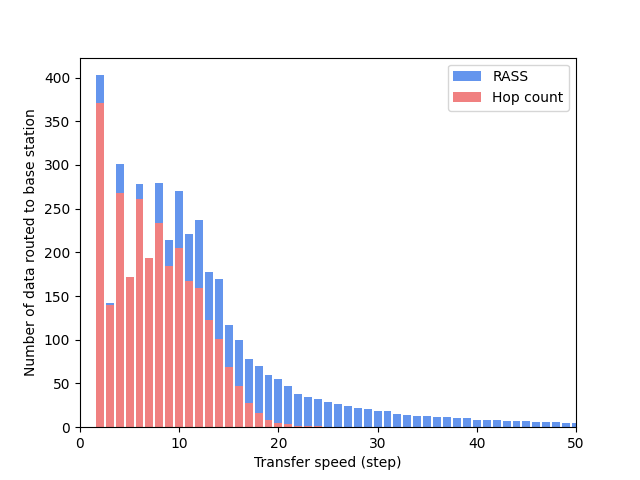
\includegraphics[width=0.75\textwidth]{images/random_speed.png}
        \label{results:random_100_speed}
        }
    \caption{(a) Reliability over time (b) Distribution of transfer speeds. Performance comparison of RASS, hop count and stigmergy in a dynamic random search topology.}
    \label{results:dynamicTopologyRandom}
    \vspace{-2mm}
\end{figure}

% \begin{figure*}
%     \centering
%     \begin{subfigure}{0.8\textwidth}
%         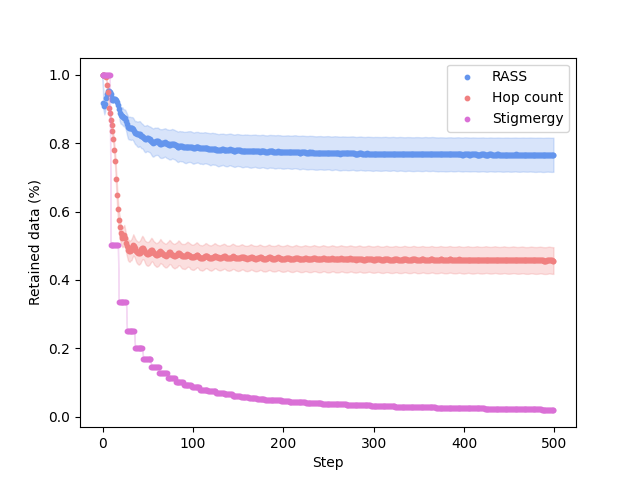
\includegraphics[width=\textwidth]{images/grid_reliability.png}
%         \caption{Reliability over time}
%         \label{results:grid_100_reliability}
%     \end{subfigure}
%     \begin{subfigure}{0.8\textwidth}
%         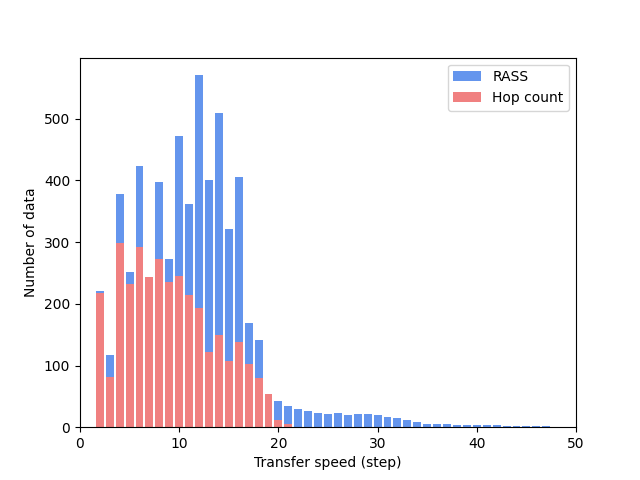
\includegraphics[width=\textwidth]{images/grid_speed.png}
%         \caption{Distribution of transfer speeds}
%         \label{results:grid_100_speed}
%     \end{subfigure}
%     \caption{Performance comparison of RASS, hop count and stigmergy in a static grid-like topology.}
%     \label{results:staticTopology}
%     \vspace{-2mm}
% \end{figure*}

% \begin{figure*}
%     \centering
%     \begin{subfigure}{0.8\textwidth}
%         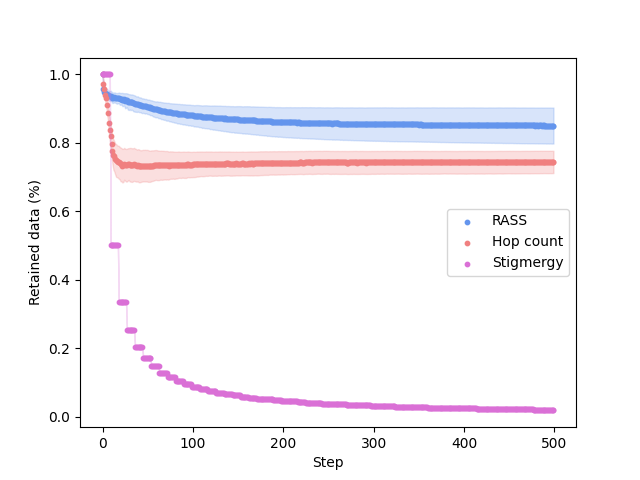
\includegraphics[width=\textwidth]{images/scale_reliability.png}
%         \caption{Reliability over time}
%         \label{results:scale_100_reliability}
%     \end{subfigure}
%     \begin{subfigure}{0.8\textwidth}
%         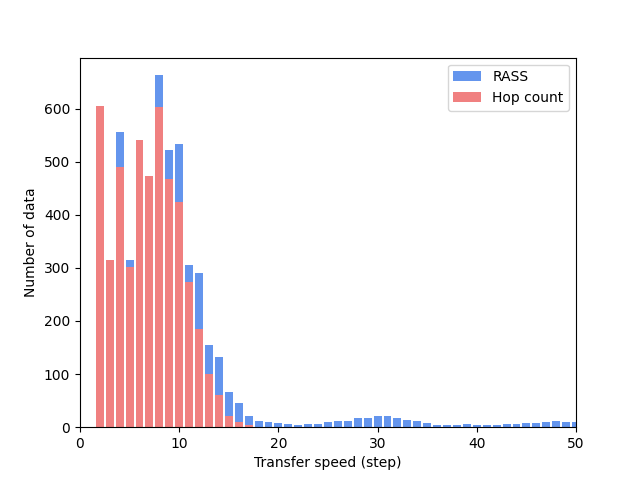
\includegraphics[width=\textwidth]{images/scale_speed.png}
%         \caption{Distribution of transfer speeds}
%         \label{results:scale_100_speed}
%     \end{subfigure}
%     \caption{Performance comparison of RASS, hop count and stigmergy in a static Scale Free topology.}
%     \label{results:staticTopologyScale}
%     \vspace{-2mm}
% \end{figure*}

% \begin{figure*}
%     \centering
%     \begin{subfigure}{0.8\textwidth}
%         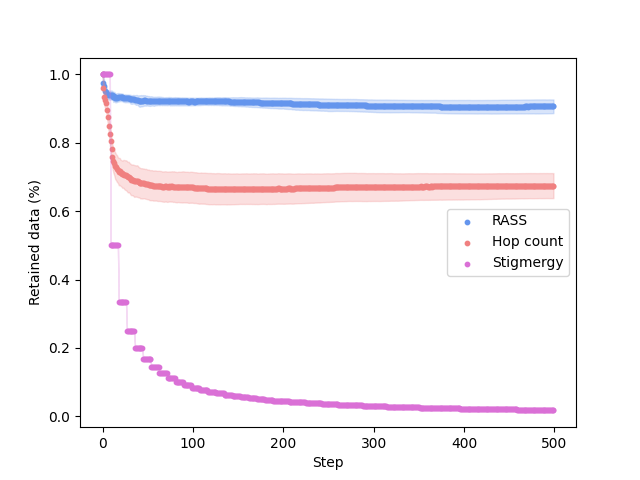
\includegraphics[width=\textwidth]{images/lennard_reliability.png}
%         \caption{Reliability over time}
%         \label{results:lennard_100_reliability}
%     \end{subfigure}
%     \begin{subfigure}{0.8\textwidth}
%         \includegraphics[width=\textwidth]{images/lennard_speed.png}
%         \caption{Distribution of transfer speeds}
%         \label{results:lennard_100_speed}
%     \end{subfigure}
%     \caption{Performance comparison of RASS, hop count and stigmergy in a dynamic Lennard-Jones topology.}
%     \label{results:dynamicTopologyLennard}
%     \vspace{-2mm}
% \end{figure*}

% \begin{figure*}
%     \centering
%     \begin{subfigure}{0.8\textwidth}
%         \includegraphics[width=\textwidth]{images/random_reliability.png}
%         \caption{Reliability over time}
%         \label{results:random_100_reliability}
%     \end{subfigure}
%     \begin{subfigure}{0.8\textwidth}
%         \includegraphics[width=\textwidth]{images/random_speed.png}
%         \caption{Distribution of transfer speeds}
%         \label{results:random_100_speed}
%     \end{subfigure}
%     \caption{Performance comparison of RASS, hop count and stigmergy in a dynamic random search topology.}
%     \label{results:dynamicTopologyRandom}
%     \vspace{-2mm}
% \end{figure*}

\begin{table}[htpb]
\centering
\caption{Average transfer speed and average individual memory usage with different topologies}
\label{table:speed}
\def\arraystretch{1.5}
\setlength{\tabcolsep}{8pt}
\begin{tabular}{llcc}
\hline
\multicolumn{1}{c}{\textit{\textbf{Topology}}} &
  \multicolumn{1}{c}{\textit{\textbf{Algorithm}}} &
  \textit{\textbf{\begin{tabular}[c]{@{}c@{}}Transfer speed (hops)\end{tabular}}} \\ \hline

\multirow{3}{4cm}{\textbf{Grid-like}}    & RASS      & 11.45  \\ \cline{2-3} 
                                         & Hop-Count & 9.11   \\ \cline{2-3} 
                                         & Stigmergy & N.A.  \\ \hline
\multirow{3}{4cm}{\textbf{Scale-Free}}   & RASS      & 11.44    \\ \cline{2-3} 
                                         & Hop-Count & 6.85     \\ \cline{2-3} 
                                         & Stigmergy & N.A.   \\ \hline
\multirow{3}{4cm}{\textbf{Lennard-Jones}}& RASS      & 12.51    \\ \cline{2-3} 
                                         & Hop-Count & 7.32     \\ \cline{2-3} 
                                         & Stigmergy & N.A.   \\ \hline
\multirow{3}{4cm}{\textbf{Random Search}}& RASS      & 12.68    \\ \cline{2-3} 
                                         & Hop-Count & 7.76    \\ \cline{2-3} 
                                         & Stigmergy & N.A.  \\ \hline
\end{tabular}
\end{table}


\section{Physical experiments}

To assess its real-world applicability, we also tested RASS with a swarm of 5 physical robots using a static topology illustrated in fig. \ref{cogniflyExperiment1} and fig. \ref{cogniflyExperiment2}. 

\begin{figure}[htbp]
	\centering
    \includegraphics[width=0.7\columnwidth]{images/physical-topology.png}
    \caption{Topology of the 3x3m environment with 4 drones, a base station and a radiation source used in the physical experiments.}
    \label{cogniflyExperiment1}
\end{figure}

\begin{figure}[htbp]
	\centering
    \includegraphics[width=0.64\columnwidth]{images/cognifly.jpg}
    \caption{Picture of the 3x3m environment with 4 drones, a base station and a radiation source used in the physical experiments.}
    \label{cogniflyExperiment2}
\end{figure}

The goal was showing that the algorithm was easily transferable to physical robots and that it behaves the ways it is intended to. In this particular topology, one route is clearer safer than the other. We expect RASS to choose the safest one even if it is not necessarily the shortest towards the base station. We performed 3 runs of the RASS algorithm and compared its performance with the hop-count based algorithm. Results are presented in fig. \ref{results:physicalRelaibility}.

\begin{figure}[htbp]
	\centering
    \includegraphics[width=0.90\columnwidth]{images/reliability.png}
    \caption{Evolution of reliability over time on the physical experiments}
    \label{results:physicalRelaibility}
\end{figure}


Again, results show that RASS offers better reliability results than the hop-count based algorithm. RASS' percentage of retained data is about 75\%, what was expected in the particular topology. Indeed, one of the four robots is located on the radiation source and therefore looses almost all its data items due to corruption. The other three robots are able to route their data items using the safe route. On the other hand, the hop-count based algorithm looses a bit more than 50\% of the data items as the two possible routes towards the base station as taken analogously, regardless of the risk. It is true that very few conclusions can be drawn by the physical experiments as the swarm size is very limited and the topology chosen arbitrarily. However, the main motivation was showing that the algorithm, as it is, can be easily implemented on physical robots and can run the way it is intended to. Of course, further physical experiments, with a greater number of robots and more realistic topologies, will need to be carried to assess RASS' performance in real-world scenarios.

\section{Conclusion}

We presented RASS, a fully decentralized risk-aware storing and routing algorithm. By leveraging a fitness policy based on both hop count and risk, RASS is able to choose the appropriate agents through which to route data items towards the base station. Results from our experiments show that RASS consistently outperforms the hop-count based algorithm in terms of reliability across different topologies, both static and dynamic. RASS also performed well in physical experiments where the main motivation was showing that the algorithm, as it is, can be easily implemented on physical robots and can run the way it is intended to.

Additional experiments on larger swarms of robots and in more diverse scenarios will be necessary to assess RASS' performance in real world missions. Also, some additional work includes understanding the impact of the communication network assumptions on the performance of RASS. For example, a network where there exists only a few routes towards the base station and where one is clearly safer than the other is, of course, well suited for our algorithm. On the other hand, the value of RASS should decrease in well-connected networks where the radiation sources are only located at the periphery of the network (far from the base station). Indeed, in this particular scenario, because data naturally moves away from the risk, RASS' risk awareness shouldn't improve noticeably the network's reliability.


             % Second thème (Doctorat) ou "Résultats théoriques et expérimentaux" (Maîtrise).

% \Chapter{DORA: Distributed Online Risk-Aware Explorer}\label{sec:Theme1}
 

% \section{Abstract}
% Exploration of unknown environments is an important challenge in the field of robotics. While a single robot can achieve this task alone, evidence suggests it could be accomplished more efficiently by groups of robots, with advantages in terms of terrain coverage as well as robustness to failures. Exploration can be guided through belief maps, which provide probabilistic information about which part of the terrain is interesting to explore (either based on risk management or reward). This process can be centrally coordinated by building a collective belief map on a common server. However, relying on a central processing station creates a communication bottleneck and single point of failure for the system. In this paper, we present Distributed Online Risk-Aware (DORA) Explorer, an exploration system that leverages decentralized information sharing to update a common risk belief map. DORA-Explorer allows a group of robots to explore an unknown environment discretized as a 2D grid with obstacles, with high coverage while minimizing exposure to risk, effectively reducing robot failures.

% \section{Introduction}

% The exploration of unknown environments is at the core of numerous
% robotic applications from search-and-rescue operations
% \cite{matos2016multiple} to space
% missions~\cite{fong2005interaction}. The problem has been mostly
% studied in single robot setups, but the ability to perform exploration
% with teams of robots opens the door to even more ambitious
% applications, because with proper coordination, the time required to
% explore a given environment should decrease proportionally to the
% number of robots~\cite{burgard2005coordinated}. Therefore, multi-robot
% exploration is an attractive solution to many time-critical
% applications such as search-and-rescue operations or planetary
% exploration. Moreover, multi-robot teams are usually resilient to some
% amount of robot
% failures~\cite{ramachandran2019resilience,wehbe2021probabilistic,winfield2006safety}. However,
% robot failures are still undesirable as they can affect team
% performance and should therefore be avoided, which is the main
% motivation for this work, in which we present a risk-aware exploration
% algorithm for multi-robot systems: Distributed Online Risk-Aware
% (DORA) Explorer.

% Multi-robot systems come with their own sets of constraints and
% challenges: among those, coordination and communication are the most
% relevant to the exploration problem. Without coordination, the robots
% will inevitably explore overlapping parts of the environment, leading
% to little gains in terms of efficiency compared to single-robot
% solutions. While the coordination could be optimally orchestrated from
% a central computing station, such a solution would require a perfect
% connectivity maintenance with each robot and a high communication
% bandwidth since the robots would need to send their observations and
% receive their commands. This motivates the need for a decentralized
% exploration algorithm relying only on local computation onboard the
% robots and communication with their neighbours. To the best of our knowledge, there exists no risk-aware collaborative
% exploration algorithm that relies solely on local or shared
% information. Therefore, in this paper, we make the following
% contribution to the field of multi-robot exploration: \textit{A
%   decentralized exploration algorithm leveraging distributed belief
%   maps (DBMs) to maximize coverage and decrease robot failure
%   probability using risk-awareness.} To
% evaluate this system, we test it on the specific problem of
% \emph{hazard mapping} in a 2D world discretized as a grid, in which a
% multi-robot team simultaneously explores a dangerous environment and
% collaborates to avoid hazardous locations as well as obstacles. We validate our approach in a physics-based simulator, ARGoS
% \cite{Pinciroli:SI2012}, in which we define a grid-based environment
% with multiple radiation sources. We then test it on physical
% robots. In our experiments, the belief of each cell models the
% likelihood of robot failure at that point in space due to ionizing
% radiation. It is worth noting that the risk of failure could originate
% from any other danger type, such as fire, rough terrain, etc.

% \section{Related Work and Background}
% Distributed sensing and information sharing is not trivial, especially considering
% the challenges of consistency and partial connectivity among the
% robotic teams~\cite{amigoni2017multirobot,otte2018emergent}. The virtual stigmergy
% presented in \cite{pinciroliTuple2016} and implemented in the Buzz
% programming language \cite{pinciroliBuzz2016} achieves consensus among
% a group of robots using Conflict-free Replicated Data Types (CRDTs),
% represented as key-value pairs shared and replicated among the swarm members. This sort of shared data structure is
% particularly relevant for belief maps, since it is easy to assign a
% unique key to each cell based on its location.  In the virtual
% stigmergy, data is shared on writing and reading the CRDT, with the
% additional updates on read improving the robustness to temporary
% disconnections and message drops. This solution differs from
% distributed hash tables, which require a complete view of the system
% at every point in time. Essentially, information updates are propagated throughout the swarm using the stigmergy whenever it is possible. In this sense, it offers high availability while settling for eventual data consistency. Other distributed data storage approaches such
% as SwarmMesh \cite{majcherczykSwarmmesh2020} store data in different
% locations based on a fitness function instead of replicating them on
% all robots. This allows the storage of more data with less
% communication, but robots are less likely to have access to the latest
% values.

% Belief maps are a simple yet powerful tool for robotic exploration
% because they can represent an environment with a 2D cell grid. They
% are a generalization of occupancy maps: instead of storing only one
% bit per cell to indicate the presence of an obstacle/danger, they
% store obstacle/danger likelihoods and offer significant improvements
% for exploration \cite{stachnissMappingExplorationMobile2003}. In the
% field of multi-robot exploration, early techniques leveraging belief
% maps date back as far as twenty years
% \cite{kobayashiSharingExploringInformation2002,kobayashiDeterminationExplorationTarget2003},
% but they rely on a fixed grid size and are tested only with two
% robots. More recent works also leverage belief maps for multi-robot
% exploration. For example,
% in~\cite{indelmanCooperativeMultirobotBelief2018}, the robots consider
% both the current beliefs and the expected beliefs from future
% observations to coordinate their exploration. Grid maps and belief
% maps are also widely used to train deep reinforcement learning
% exploration policies
% \cite{hanGridWiseControlMultiAgent,panovGridPathPlanning2018}, but they often rely on a trial and error process which may select actions leading to failures \cite{garciaSafeExplorationState2012,andersenSafeReinforcementlearningIndustrial2020}.

% To provide more insight into our claim that there are no risk-aware collaborative exploration strategies in  the literature, it should be noted that risk-awareness has indeed been used in some swarm systems to improve robustness. For example, several path planners based on Markov Decision Processes \cite{undurti2010online,thiebaux2016rao,xiao2020robot} take into account risk and have useful definitions of it. Another interesting idea for risk awareness is proposed in \cite{ono2008efficient,vitus2011feedback}, where a "risk budget" is allocated to their agents, allowing them to optimize a balance between risk and reward to guide robots. However, these systems assume a knowledge of the global state of the environment, which is unavailable when exploring unknown environments. Furthermore, most are only applied to single-robot systems. In SPIDER \cite{hunt2020spider}, multiple agents are tasked with chain formation in dangerous environments. They adapt to varying levels of risk to be resilient to significant failures and member losses. However, their task is significantly different from DORA Explorer's objectives.

% Many distributed exploration strategies maximizing the amount of
% covered terrain have been proposed. The first approaches to stand out
% in this regard are Voronoi-based coverage control
% techniques~\cite{luo2019voronoi,santos2019decentralized}. A second
% method covers time-varying domains, in which points in the
% covered region can become more or less interesting to explore,
% therefore prompting a change in the coverage function
% \cite{santos2019decentralized,xu2019multi}. Another method to optimize
% coverage is Frontier-Based Exploration (FBE)
% \cite{yamauchi1998frontier} of which many variations have been
% developed, such as those based on Particle Swarm Optimization
% \cite{wang2011frontier} or the Wavefront Frontier Detector
% \cite{topiwala2018frontier}. However, none of these strategies take
% risk into account. Therefore, the
% exploration strategy implemented in this paper takes inspiration of
% the multi-robot control algorithm presented in
% \cite{dames2012decentralized,schwagerMultirobotControlPolicy2017}
% which maximizes the information gain during exploration in the
% presence of unknown hazards. However, this optimal algorithm has a
% very high computational complexity and could benefit from approximations.


% \section{System Model}
% DORA-Explorer builds on the previously mentioned approaches and addresses some of their shortcomings, namely by leveraging risk awareness to provide better efficiency when exploring hazardous environments which are not constrained to fixed sizes. Reducing the
% likelihood of robot failures is of high importance as failures lead to
% poor exploration performance. Indeed, if robots experiencing complete
% failures are not replaced, individual failures lead to lower numbers
% of robots carrying the exploration task resulting in a decrease of the exploration rate. By keeping robots operational, our
% risk-aware exploration algorithm enables the exploration of the
% environment with the contribution of all the team members. We model the 2D environment as cells forming a grid
% represented as $E \subset \mathbb{Z}^2$. The team of robots is denoted
% as the collection of agents $a_i \in A$.

% % \begin{figure*}[h]
% %     \centering
% %     % \begin{subfigure}{0.40\textwidth}
% %     %      \centering
% %     %      \includegraphics[width=\textwidth]{images/risk_aware_a.png}
% %     %      \caption{}
% %     %      \label{risk_aware_a}
% %     % \end{subfigure}
% %     % \hfill
    
    
% %     \begin{subfigure}{0.30\textwidth}
% %          \centering
% %          \includegraphics[width=\textwidth]{images/risk_aware_b.png}
% %          \caption{}
% %          \label{risk_aware_b}
% %     \end{subfigure}
% %     \hfill
% %     \begin{subfigure}{0.30\textwidth}
% %          \centering
% %          \includegraphics[width=\textwidth]{images/risk_aware_c.png}
% %          \caption{}
% %          \label{risk_aware_c}
% %     \end{subfigure}
% %     \hfill
% %     \begin{subfigure}{0.30\textwidth}
% %          \centering
% %          \includegraphics[width=\textwidth]{images/risk_aware_d.png}
% %          \caption{}
% %          \label{risk_aware_d}
% %     \end{subfigure}
% %         \caption{Risk aware exploration intuition. Fig. \ref{risk_aware_b}: Robots start exploring a hazardous environment. When a new cell is explored, the sensed radiation is used to update the DBM. Fig. \ref{risk_aware_c}: The cells have been mostly covered by the robots. Fig. \ref{risk_aware_d}: Only cells believed to be too dangerous remain unexplored.}
% %     \label{risk_aware}
% % \end{figure*}


% \subsection{Risk Modelling}
% Without loss of generality, we model risk considering point radiation
% sources, denoted by the set $S$. The intensity of each radiation
% source is given by $I_j\sim\mathcal{U}(0, 1)$. Each source's position
% is denoted by $\bm{s}_j \in E$. Given a robot $a_i$'s discrete
% position $\bm{x}_i \in E$, the perceived radiation level by that robot coming from radiation source $\bm{s}_j$ is given by:

% \begin{equation}
%     r_{\bm{s}_j}(\bm{x}_i) = \frac{I_j}{1 + \lambda\rho^2}
%     \label{eq:radiation}
% \end{equation}

% which decays as the distance $\rho$ between $\bm{s}_j$ and $\bm{x}_i$
% increases, and $\lambda$ is a decay constant. Measurement noise is
% accounted for in the form of a Gaussian background radiation
% $b \sim \mathcal{N}(0, 0.05)$. The total radiation perceived by a robot is:

% \begin{equation}
%     r(\bm{x}_i) = b + \sum_{\bm{s}_j \in S} r_{\bm{s}_j}(\bm{x}_i)
% \end{equation}

% Robots are only able to sense the radiation level associated with
% their current position using an onboard sensor. They do not hold any
% knowledge of where the radiations sources are located in the
% environment. For the following definitions, it should be noted that
% $r_{s_j}: E \rightarrow [0, 1]$.  Let
% the event of robot $a_i$ failing be $f_i=1$, the probability of such a
% failure due to an individual source of radiation follows a Bernoulli
% distribution:
% $\mathbb{P}(f_i = 1 | \bm{s}_j) \sim
% \mathcal{B}(r_{\bm{s}_j}(\bm{x}_i))$. We assume that the sources of
% radiation affect the robots independently, so the probability of a
% robot failing due to the combined effect of all radiation sources is:

% \begin{equation}
%     \mathbb{P}(f_i = 1 | S) = 1 - \prod_{\bm{s_j} \in S} (1 - \mathbb{P}(f_i = 1 | \bm{s}_j))
%     \label{eq:failure}
% \end{equation}

% \subsection{Information Modelling}
% The objective of exploring an unknown dynamic environment is to gain
% information about it. Moreover, this information should be as up to
% date as possible. Therefore, it is unlikely that visiting a recently
% explored cell will yield any significant gain as the information
% should not have changed drastically. Conversely, exploring areas
% visited long ago should yield a greater information gain, and
% unvisited areas should provide the highest information gain. The last
% time of exploration $t_\epsilon$ by robot $a_i$ of a cell at position
% $\bm{x}_i$ can be represented by the scalar field
% $\epsilon(\bm{x}_i) = t_\epsilon$. Let $u_i=1$ be the event of robot
% $a_i$ finding useful information in a cell and
% $\Delta t = t-t_\epsilon$ the time elapsed since the cell was last
% visited, with $t$ being the current time. Then, the probability of
% \textit{not} finding useful information
% $\mathbb{P}(u_i=0 | f_i=0, \Delta t)$ can be modelled as an
% exponential distribution with the following probability density
% function:

% \begin{equation}
%     f(\Delta t;\omega) = \omega e^{-\omega\Delta t}
%     \label{eq:information}
% \end{equation}

% where $\omega$ is the rate parameter of the distribution. In words,
% the longer the cell has not been visited, the higher the chance
% something has changed and consequently the lower the chance of not
% finding useful information. It follows that the probability of finding
% useful information if the robot is operational can be expressed as:

% \begin{equation}
%     \mathbb{P}(u_i=1 | f_i=0, \Delta t) = 1 - \mathbb{P}(u_i=0 | f_i=0, \Delta t)
%     \label{eq:usefulInformation}
% \end{equation}

% Intuitively, no information can be acquired by failed robots, which
% can be expressed as:

% \begin{equation}
%     \mathbb{P}(u_i=1 | f_i=1) = 0
%     \label{eq:informationFailure}
% \end{equation}

% \subsection{Distributed Belief Map}
% To implement a DBM, we use the virtual
% stigmergy~\cite{pinciroliTuple2016} from the
% Buzz~\cite{pinciroliBuzz2016} programming language. Because
% $r(\bm{x}_i)$ and $\epsilon(\bm{x}_i)$ are both scalar fields, they
% lend themselves particularly well to being stored in a CRDT at a low
% cost. At each time step, the robots store their values of
% $r(\bm{x}_i)$ and $\epsilon(\bm{x}_i)$ in their respective
% stigmergies.  The inputs to both fields are used as keys in the distributed belief map (more precisely, a concatenation of $\bm{x}_{i;x}$ and $\bm{x}_{i;y}$). This
% means that the cost of storing the information for a given time step
% is very low, especially as the keys consist of a few characters and
% the values are floating point numbers. Storing the information into
% the DBM via the virtual stigmergy allows robots to share their
% observations as it is accessible by every robot in the system. Thus, a
% robot visiting a cell for the first time could still have information from
% which to compute a good control policy if this cell was previously
% visited by another robot. In the event of a collision in the stigmergy
% (when robots write to the same key in the same $t$), the robot making the latest observation updates the table and the corresponding entry is shared back to the other robots. When a robot writes to a key already present
% in the stigmergy (from a previous time step), the new data is merged
% with an average and the result is propagated. A running average was used to update the belief map because of the noisy readings. The stigmergies do not directly store probabilities
% and thus cannot be strictly considered as belief maps
% \cite{kobayashiSharingExploringInformation2002}.  However,
% $r(\bm{x}_i)$ and $\epsilon(\bm{x}_i)$ always vary in the same
% directions as $\mathbb{P}(f_i = 1 | S)$ and
% $\mathbb{P}(u_i=1 | f_i=0, \Delta t)$ respectively, so they can be
% used to formulate a control law based on the optimization of these
% probability functions.


% \subsection{Control Law}
% We assume that robots can be controlled through a position-based
% control law. The best control policy should attempt to minimize
% probability of failure and to maximize the information gain. While the
% directions achieving these individual objectives might be at odds in
% the short term, they are in fact complementary in the long term
% because no information can be gained if a robot failed, as defined by
% \eqref{eq:informationFailure}, which means that avoiding danger
% implicitly leads to more opportunities of gaining information
% \cite{schwagerMultirobotControlPolicy2017}.

% \begin{figure}[h]
% 	\centering
%     \includegraphics[width=0.90\columnwidth]{images/Moore.png}
%     \caption{$\bm{x}_i$'s neighborhood. $\bm{n}_{i,0} = (-1, 1)$ is neighbor 0's offset from $\bm{x}_i$.}
%     \label{neighborhood}
% \end{figure}

% For a robot at a given position $\bm{x}_i$, the directions where the
% risk is minimized and the information gain is maximized are
% respectively $\bm{\nabla}r(\bm{x}_i)$ and
% $\bm{\nabla}\epsilon(\bm{x}_i)$, also denoted as $\bm{\nabla}_{r;i}$
% and $\bm{\nabla}_{\epsilon;i}$. Calculating these globally at every
% time step is too computationally expensive
% \cite{dames2012decentralized,schwagerMultirobotControlPolicy2017}. Instead,
% we compute them locally in a Moore neighborhood $\nu$ centered on
% $\bm{x}_i$ as shown in Fig. \ref{neighborhood} where each neighboring
% cell $\bm{n}_{i,j} \in \nu$ is a vector in $\mathbb{Z}^2$ representing
% an offset from $\bm{x}_i$. We then have:

% \begin{equation}
%     \bm{\nabla}_{r;i} = \sum_{\bm{n}_j \in \nu}\frac{\partial r}{\partial \bm{n}_{i,j}} \bm{\hat{n}}_{i,j} \text{ , with } \frac{\partial r}{\partial \bm{n}_{i,j}} = r(\bm{x}_i) - r(\bm{n}_{i,j})
%     \label{eq:gradient_risk}
% \end{equation}

% \begin{equation}
%     \bm{\nabla}_{\epsilon;i} = \sum_{\bm{n}_j \in \nu}\frac{\partial \epsilon}{\partial \bm{n}_{i,j}} \bm{\hat{n}}_{i,j} \text{ , with } \frac{\partial \epsilon}{\partial \bm{n}_{i,j}} = \epsilon(\bm{x}_i) - \epsilon(\bm{n}_{i,j})
%     \label{eq:gradient_exploration}
% \end{equation}

% % \begin{equation}
% %     \frac{\partial r}{\partial \bm{n}_{i,j}} = r(\bm{x}_i) - r(\bm{n}_{i,j})
% %     \label{eq:neighbor}
% % \end{equation}

% % \begin{equation}
% %     \bm{\nabla}_{r;i} = \sum_{\bm{n}_j \in \nu}\frac{\partial r}{\partial \bm{n}_{i,j}} \bm{\hat{n}}_{i,j}
% %     \label{eq:gradient}
% % \end{equation}

% % \begin{equation}
% %     \frac{\partial \epsilon}{\partial \bm{n}_{i,j}} = \epsilon(\bm{x}_i) - \epsilon(\bm{n}_{i,j})
% %     \label{eq:neighbor}
% % \end{equation}

% % \begin{equation}
% %     \bm{\nabla}_{\epsilon;i} = \sum_{\bm{n}_j \in \nu}\frac{\partial \epsilon}{\partial \bm{n}_{i,j}} \bm{\hat{n}}_{i,j}
% %     \label{eq:gradient}
% % \end{equation}

% where $\bm{\hat{n}}$ is the unit form of $\bm{n}$. Neighboring cells that have never been visited before are simply ignored when determining the gradients. If none of the neighboring cells have been explored yet, or if the computed direction is null, the robot simply moves forward until it's able to compute a meaningful direction. The movement vector $\bm{m}_i \in \mathbb{R}^2$ for the next time step
% gives a good approximation for short term trajectory planning and is given by:

% \begin{equation}
%     \bm{m}_i = \alpha\bm{\nabla}_{r;i} + \beta\bm{\nabla}_{\epsilon;i} + \gamma\bm{o}_i
%     \label{eq:movement}
% \end{equation}

% where $\alpha, \beta, \gamma$ are respectively the risk avoidance,
% exploration and obstacle avoidance control gains. The parameters can
% be adjusted arbitrarily; setting them to zero removes the effect
% of the corresponding control law. The obstacle avoidance vector was
% included to insure robustness and is taken from
% \cite{shahriari2018lightweight}. With $\bm{\hat{m}_i}$ being the
% normalized vector movement and $k$ a speed constant, the control law
% for an agent $a_i$ at time step $t$ is expressed as:

% \begin{equation}
%     \bm{x}_i^{t+1} = \bm{x}_i^t + k \bm{\hat{m}}_i^t
%     \label{eq:control}
% \end{equation}

% A constant search speed enables a fair comparison with the baselines detailed in section \ref{experimentSetup} as the exploration capabilities of the robots remain the same across the algorithms.

% \subsection{Implementation}
% The DBMs and the control law previously described are combined to create the behavior of an agent. At every
% time step, the information from the DBMs is used to determine the
% agent's next movement. The DBMs are then updated with the new
% information gained. Global exploration efficiency emerges through the
% exchange of information through the stigmergies, but no explicit
% coordination is required otherwise. Unlike FBE algorithms, DORA-Explorer never
% stops exploring the environment even if all cells are covered, as
% information could be gained by visiting "old" cells. If
% $\|\bm{\hat{m}}_i\|$ is too small, the agents move forward to avoid
% stagnation.

% \begin{algorithm}
% \small
% \SetAlgoLined
% \DontPrintSemicolon
%  $\bm{x} \leftarrow random\_coordinates$\;
%  \While{True}{
%   $\nabla_r, \nabla_e \longleftarrow (0, 0), (0, 0)$\;
%   \;
%   \For{$n \in \nu$}{
%     $\nabla_r \leftarrow \nabla_r + (r\_stig[\bm{x}] - r\_stig[\bm{n}]) \cdot normalize(\bm{n})$\;
%     $\nabla_e \leftarrow \nabla_e + (e\_stig[\bm{x}] - e\_stig[\bm{n}]) \cdot normalize(\bm{n})$\;
%   }
%   \;
%   $\bm{m} \leftarrow \alpha \cdot \nabla_r + \beta \cdot \nabla_e + \gamma \cdot compute\_avoidance(sensors)$\;
%   $\bm{x} \leftarrow \bm{x} + k \cdot normalize(\bm{m})$\;
%   $r\_stig[\bm{x}], e\_stig[\bm{x}] \leftarrow get\_radiation(), time()$\;
%  }
%  \caption{DORA Execution Loop}
%  \label{alg:dora}
% \end{algorithm}


% % \begin{figure*}
% %      \centering
% %      \begin{subfigure}{0.30\textwidth}
% %          \centering
% %          \includegraphics[width=\textwidth]{images/risk_aware_b.png}
% %          \caption{}
% %          \label{risk_unaware_a}
% %      \end{subfigure}
% %      \begin{subfigure}{0.30\textwidth}
% %          \centering
% %          \includegraphics[width=\textwidth]{images/risk_unaware_a.png}
% %          \caption{}
% %          \label{risk_unaware_b}
% %      \end{subfigure}
% %         \caption{Exploration without risk awareness. Fig. \ref{risk_unaware_a}: Robots start exploring but are unable to sense environmental radiation. The only driving force of the algorithm is exploring new cells. Fig. \ref{risk_unaware_b}: Robots fail because they do not discriminate between safe and dangerous cells. Exploration is carried out fewer robots. Exploration efficiency drastically decreases and large areas of the environment remain uncovered.}
% %         \label{risk_unaware}
% % \end{figure*}

% % \begin{figure*}[h]
% %     \centering
% %     % \begin{subfigure}{0.40\textwidth}
% %     %      \centering
% %     %      \includegraphics[width=\textwidth]{images/risk_aware_a.png}
% %     %      \caption{}
% %     %      \label{risk_aware_a}
% %     % \end{subfigure}
% %     % \hfill
% %     \begin{subfigure}{0.30\textwidth}
% %          \centering
% %          \includegraphics[width=\textwidth]{images/risk_aware_b.png}
% %          \caption{}
% %          \label{risk_aware_b}
% %     \end{subfigure}
% %     \hfill
% %     \begin{subfigure}{0.30\textwidth}
% %          \centering
% %          \includegraphics[width=\textwidth]{images/risk_aware_c.png}
% %          \caption{}
% %          \label{risk_aware_c}
% %     \end{subfigure}
% %     \hfill
% %     \begin{subfigure}{0.30\textwidth}
% %          \centering
% %          \includegraphics[width=\textwidth]{images/risk_aware_d.png}
% %          \caption{}
% %          \label{risk_aware_d}
% %     \end{subfigure}
% %         \caption{Risk aware exploration intuition. Fig. \ref{risk_aware_b}: Robots are dispatched in a hazardous environment and start exploring. When a new cell is explored by a robot, the sensed radiation is used to update the DBM. Fig. \ref{risk_aware_c}: The environment has been largely covered by the robots. Fig. \ref{risk_aware_d}: Only the cells believed to be too dangerous remain unexplored.}
% %     \label{risk_aware}
% % \end{figure*}

% \subsection{Scalability}
% \label{subsec:scalability}
% To achieve scalability to a high number of agents and to large
% environments, DORA-Explorer must have low communication and computational costs. Lowering the communication costs associated
% with sharing the DBM can be done by using the virtual
% stigmergy, which is designed to limit information exchange to read or
% write operations only on the requested data. Because DORA-Explorer relies
% solely on local information, the data transfer cost $D(A, \nu, E)$ for
% an agent at a given time step is independent from the total number of
% agents in $A$ and from the size of the environment $E$. For a
% neighboring cell $\bm{n}_{i,j} \in \nu$, 2 stigmergy read operations
% are needed per time step: one each to read $r(\bm{n}_{i,j})$ and
% $\epsilon(\bm{n}_{i,j})$. In the same time step, the agent updates
% $r(\bm{x}_i)$ and $\epsilon(\bm{x}_i)$ after it has moved to a new
% location, which requires 2 stigmergy write operations. Each stigmergy
% access requires only a few tens of bytes of data transfer for the key
% and value. This mostly constant data quantity is represented as $d$,
% we have $D(A, \nu, E) = 2d(|\nu| + 1)$. Similarly, the computational
% cost $C(A, \nu, E)$ for the same agent at the same time step is kept
% very low because of the reliance on local information only. Each time
% step requires to compute 2 gradients, and referring to
% \eqref{eq:gradient_risk}, \eqref{eq:gradient_exploration}, \eqref{eq:movement} and
% \eqref{eq:control} we have that $C(A, \nu, E) = 12|\nu|+7$. The costs
% related to $\bm{o}_i$ have been excluded from this analysis as
% obstacle avoidance is not a critical part of DORA-Explorer. The step-wise communication
% and computational costs for an agent are thus
% both bounded by:

% \begin{equation}
%     D(A, \nu, E) \text{ and } C(A, \nu, E) \in \Theta(|\nu|)
%     \label{eq:costs}
% \end{equation}

% Such low costs mean that DORA-Explorer should scale well to a large number of
% robots and should enable real time computation for even very limited computational platforms.


% \section{Simulations}
% \subsection{Experimental setup}
% \label{experimentSetup}

% We tested our system through simulations in ARGoS
% \cite{Pinciroli:SI2012}, which is an open-source physics-based
% simulation environment designed for robotic swarms. The agents we used
% in the simulation are KheperaIV robots
% \cite{kteam2021kheperaiv}. These are small round robots (140mm of
% diameter) equipped with 8 infrared proximity sensors spread evenly
% around their frame to perform obstacle avoidance. The
% agents are programmed in Buzz to facilitate swarm
% management and interaction.

% \begin{figure}[h]
% 	\centering
%     \includegraphics[width=0.95\columnwidth]{images/argos.png}
%     \caption{$400 \text{m}^2$ environment in the ARGoS simulator with 20 KheperaIV robots. Cylinders are radiation sources and boxes are random obstacles.}
%     \label{argos}
% \end{figure}

% We deployed a set of N = \{10, 15, 20\} robots in a simulated
% environment of 20x20m with set of 2 radiation sources. The environment is discretized into 400 cells, where each cell of the grid is 1x1m large. The robots'
% initial positions are chosen randomly. We arbitrarily set $\lambda$ from
% \eqref{eq:radiation} to be 5 as it was providing an adequate decay speed in relation with the size of our environment: The robots would generally fail in a 3m radius around the radiation sources. The speed constant $k$ from \eqref{eq:control} is set to
% $20$ to match the maximal speed of the KheperaIV robots. Because no information gain can be achieved by a failed robot as
% seen in \eqref{eq:informationFailure}, failure must be avoided. This
% leads to choosing $\alpha >= \beta$ in \eqref{eq:control}. For our
% experiments, we set $\alpha=2, \beta=1$ and $\gamma=1$. The robots are
% all given a random initial orientation. Radiation sensing is emulated
% by an ARGoS controller reading the randomly generated radiation
% sources. Failures are randomly triggered by using \eqref{eq:failure}:
% if $f_i=1$, the robot stops exploring. We added 5 randomly distributed
% 0.8m x 0.8m obstacles to each simulation run to verify the robot's ability to
% perform exploration even in cluttered environments.



% We performed 50 simulation runs over 300 steps of the DORA-Explorer
% algorithm. Each time step lasts 0.8s. To assess DORA-Explorer's performance, we compare it to the results
% obtained by a random walk algorithm and by a FBE algorithm. The
% latter's key principle is to assign one of three states (explored,
% frontier, unexplored) to the cells constituting the environment and to
% coordinate the robots to explore the regions near the frontier,
% thereby expanding them and eventually achieving full map coverage. To
% implement it, we adapted the algorithm from
% \cite{yamauchi1998frontier} by having the robots share an exploration
% map through a virtual stigmergy. The comparison with frontier exploration is
% particularly relevant because it allows us to gain insights on our
% algorithm performance in terms of terrain coverage compared to an
% algorithm which was specifically designed to maximize this
% objective. We also compare DORA-Explorer with a random walk algorithm as a
% baseline it absolutely needs to outperform. These two baselines are
% commonly used for the exploration of unknown environments in the field
% of swarm robotics. They do not take risk into account, but to the best
% of our knowledge, no other existing swarm exploration strategy does. To address this issue, we could have modified the baselines to take risk into account, but chose against it. Adding risk thresholds for movement could be considered. However, because of the randomness, determining the optimal threshold for this value might be hard to do. Additionally, if the robots find themselves in radiation hotspots, they might remain stuck in these locations because all surrounding cells will a have similar/equal risk which is too high to allow movement, resulting in fatal stagnation. Obstacle avoidance algorithms could have also been adapted to a risk avoidance context and serve as a baseline for DORA-Explorer. However, taking account of varying levels of risk would have been challenging. Again, it is hard to determine the threshold on risk level after which a cell should be considered as containing an obstacle.

% % For the FBE method, a possibility would have been to treat radiation sources as obstacles and use an obstacle avoidance mechanism to stay away from them.
% % However, there are two issues with this. First, these algorithms mostly focus on avoiding one obstacle at a time (the closest one), and therefore do not consider the effect of combined obstacles. This would not make sense anyway: two obstacles cannot be at the same location, while radiation sources can have a combined effect in one location. Second, these algorithms usually detect the presence of an obstacle in a binary way and are thus ill-suited for the presence of a gradual risk.

% The \nth{1} metric used to assess the validity of our approach is the
% number of robots which remain active (not failed) over time. This is
% perhaps the most important metric because it shows how well DORA-Explorer
% performs in terms of risk avoidance, i.e. its main objective. The
% \nth{2} metric used to evaluate the algorithms is the total number of
% cells explored by the swarm. This allows us to evaluate how well our
% algorithm performs in its objective of maximizing information gain and
% to verify that avoiding risk does not impact too much the exploration
% performance. The \nth{3} metric we studied is the communication costs of
% the algorithms, measured in KB of data transmitted per robot at
% each time step. We included this in our analysis to examine if
% the algorithms can scale to large number of robots. We also ran simulations to study the impact of the parameters $\alpha$ and $\beta$ from (\ref{eq:movement}). 

% \subsection{Results}

% \begin{figure}
%     \centering
%     \begin{subfigure}{0.48\textwidth}
%         \includegraphics[width=\textwidth]{images/explored_10.png}
%         \caption{N=10 robots}
%         \label{results:explored10}
%     \end{subfigure}
%     \begin{subfigure}{0.48\textwidth}
%         \includegraphics[width=\textwidth]{images/explored_15.png}
%         \caption{N=15 robots}
%         \label{results:explored15}
%     \end{subfigure}
%     \begin{subfigure}{0.48\textwidth}
%         \includegraphics[width=\textwidth]{images/explored_20.png}
%         \caption{N=20 robots}
%         \label{results:explored20}
%     \end{subfigure}
%     \caption{Performance comparison of DORA-Explorer, FBE and random walk for number of explored cells over time.}
    
% \end{figure}

    


% \begin{figure}
%     \centering
%     \begin{subfigure}{0.48\textwidth}
%         \includegraphics[width=\textwidth]{images/activerobots_10.png}
%         \caption{N=10 robots}
%         \label{results:failures10}
%     \end{subfigure}
%     \begin{subfigure}{0.48\textwidth}
%         \includegraphics[width=\textwidth]{images/activerobots_15.png}
%         \caption{N=15 robots}
%         \label{results:failures15}
%     \end{subfigure}
%     \begin{subfigure}{0.48\textwidth}
%         \includegraphics[width=\textwidth]{images/activerobots_20.png}
%         \caption{N=20 robots}
%         \label{results:failures20}
%     \end{subfigure}
%     \caption{Performance comparison of DORA-Explorer, FBE and random walk for number of active robots over time.}
% \end{figure}

% \begin{figure*}
%     \centering
%     \begin{subfigure}{0.48\textwidth}
%         \includegraphics[width=\textwidth]{images/heatmap_random.png}
%         \caption{Random walk}
%         \label{results:beliefrandom}
%     \end{subfigure}
%     \begin{subfigure}{0.48\textwidth}
%         \includegraphics[width=\textwidth]{images/heatmap_frontier.png}
%         \caption{FBE}
%         \label{results:belieffrontier}
%     \end{subfigure}
%     \begin{subfigure}{0.48\textwidth}
%         \includegraphics[width=\textwidth]{images/heatmap_dora.png}
%         \caption{DORA-Explorer}
%         \label{results:beliefdora}
%     \end{subfigure}
%     \caption{Radiation belief maps of the 20m x 20m environment for each exploration algorithm of one specific simulation. Blank cells are unvisited areas, red stars are the point radiation sources and grey squares are the randomly generated obstacles.}
%     \label{results:belief}
% \end{figure*}

% The following results are an average of the 50 simulation runs of each algorithm. At the beginning of the exploration process, DORA-Explorer and the baselines
% perform similarly in terms of number of cells explored as shown in
% Fig. \ref{results:explored10}, \ref{results:explored15} and
% \ref{results:explored20}. As time progresses in the same figures, FBE
% achieves a slightly higher exploration coverage than DORA-Explorer, but this
% gap in performance decreases as the number of robots increases. This
% is an expected result, because DORA-Explorer's main goal is not to achieve
% maximal coverage at all costs, unlike FBE. Both FBE and DORA-Explorer clearly
% outperform the random walk algorithm. The other trend is that adding
% more robots to the swarm results in faster exploration, with a higher
% number of cells being explored for all three algorithms after 300
% steps. This shows that DORA-Explorer scales well to large number of robots, and even gains in performance when swarm size increases, which is in line
% with the benefits associated with swarm algorithms. In terms of avoiding failures, DORA-Explorer unsurprisingly outperforms both
% FBE and the random walk, as it is its main purpose. This is shown in
% Fig. \ref{results:failures10}, \ref{results:failures15} and
% \ref{results:failures20}, where DORA-Explorer exhibits a higher level of active
% robots over time, with this difference only increasing with larger
% swarm sizes. For all values of N, there are few
% survivors for FBE, and random walks perform only slightly better, while DORA-Explorer keeps most robots alive, achieving its objective.

% Fig. \ref{results:belief} shows the DBMs obtained at the end of an
% arbitrarily selected simulation where N = 20 for each algorithm.  In
% other words, it represents which cells were explored by each algorithm
% and the sensed radiation intensity associated with them for one specific run. The random
% walk covered much fewer cells than DORA-Explorer and FBE, which both covered
% roughly the same areas of the map, with the same sections remaining
% unexplored. However, these areas remained unvisited for different
% reasons. For FBE, the parts of the environment close to the radiation
% sources remained uncovered because its agents failed when approaching
% them. In contrast, DORA-Explorer did not explore these cells because it
% \textit{avoided them}. Again, DORA-Explorer achieves very similar coverage than
% FBE but does so with less robot failures. In this particular
% simulation, DORA-Explorer finished with 18 active robots, random walk finished
% with 7, and FBE with none. 

% The results from Fig. \ref{results:communicationCosts} show the amount
% of data transferred by individual agents at each time step by both
% algorithms. We excluded the random walk algorithm from this figure as
% it does not require any coordination or communication between its
% agents. DORA-Explorer transmits more data than FBE, which was expected because
% the former shares information through two DBMs, while the latter uses
% only one. In section \ref{subsec:scalability}, we predicted that the
% amount of data transmitted at each time step would only depend on the
% size of the neighborhood used, and this is confirmed by
% Fig. \ref{results:communicationCosts}, where it remains roughly
% constant for different number of agents. The small increase in data
% transmission with increasing number of robots can be attributed to
% packet collision. Overall, the amount of required data transfer is
% small in comparison with the capacities of the KheperaIV robots which
% communicate with the 802.11 b/g WiFi protocol. 

% \begin{figure}[h]
%     \centering
%     \includegraphics[width=1\columnwidth]{images/communication.png}
%     \caption{Communication costs for DORA-Explorer and FBE}
%     \label{results:communicationCosts}
% \end{figure}

% Results from Fig. \ref{results:parameters} show the performance of DORA-Explorer with varying ratios of risk gain $\alpha$ to exploration gain $\beta$. The experiments were carried with 10 robots. Results show that the number of remaining active robots at the end of the simulation only increases with a higher ratio. This is the expected behaviour as increasing the ratio corresponds to giving more importance to the risk avoidance control law from (\ref{eq:movement}). As for the number of cells explored, the relationship is not monotonic. In our experimental setup, a ratio $\alpha / \beta = 2$ provided the best result in terms of number of cells explored. For lower ratios, the robotic team is increasingly impacted by failures which in turns worsen the exploration performance. For higher ratios, the robot are too careful and don't explore as much the environment. Choosing an adequate risk to exploration ratio is therefore important and its value will depend of the specific scenario in which the algorithm is used. 


% \begin{figure}[h]
%     \centering
%     \includegraphics[width=1\columnwidth]{images/parameters.png}
%     \caption{Performance of DORA-Explorer with varying ratios of $\alpha/\beta$}
%     \label{results:parameters}
% \end{figure}

% \section{Physical experiments}
% \subsection{Experimental setup}
% In addition to the extensive simulations conducted in ARGoS, we tested
% our system on a team of three physical KheperaIV robots in a 2x2m
% environment containing 1 point radiation source. We only used one radiation source because of the small size of the environment. The environment is discretized as a 10x10 grid, meaning that each of
% the 100 cells of the grid is 20x20cm large. Because the arena in
% which we conducted the experiments was already limited in terms of
% space we decided not to add obstacles.
% Positioning of the
% robots is done using an OptiTrack motion capture system. For outdoor
% applications where the environment is bigger, positioning of the
% robots could instead be achieved by GPS. Radiation sensing is emulated
% by an on board controller that reads the distance between the robot
% and the radiation source to determine the current radiation
% level. Failures are then triggered using equation \eqref{eq:failure},
% in other words the higher the radiation level, the higher the
% probability of failure. If a robot fails, it stops moving and as a
% result stops contributing to the exploration effort. The point
% radiation source is located in a corner of the arena and the robots
% are initially placed in the three remaining corners. The robots'
% initial orientations are chosen randomly.  We performed 5 runs over
% 200 steps of the DORA-Explorer algorithm. Each time step lasts 1s. Again, to assess DORA-Explorer's
% performance, we compare it to the results obtained by FBE and random
% walk algorithms.

%  \begin{figure}[h]
%      \centering
%      \captionsetup{belowskip=0pt}
%      \includegraphics[width=0.65\columnwidth]{images/arena.jpeg}
%      \caption{Experiments on three physical KheperaIV robots. The red canister represents the point radiation source in the environment.}
%      \label{arena}
%  \end{figure}


% \subsection{Results}
% The following results are an average of the 5 runs of each algorithm on physical robots. 

% \begin{figure}[]
%     \centering
%     \captionsetup{belowskip=-1pt}
%     \includegraphics[width=0.80\columnwidth]{images/explored_real.png}
%     \caption{Performance comparison of DORA-Explorer, FBE and random walk for number of explored cells over time on physical robots.}
%     \label{results:cells_explored_physical}
% \end{figure}

% \begin{figure}[]
%     \centering
%     \captionsetup{belowskip=-1pt}
%     \includegraphics[width=0.80\columnwidth]{images/activerobots_real.png}
%     \caption{Performance comparison of DORA-Explorer, FBE and random walk for number of active robots over time on physical robots.}
%     \label{results:active_robots_physical}
% \end{figure}

% At the beginning of the exploration process, DORA-Explorer and FBE perform
% similarly in terms of number of cells explored as shown in
% Fig. \ref{results:cells_explored_physical}. The random walk
% algorithm's exploration rate is considerably lower which can be
% attributed to the fact that some of the cells of the environment are
% visited multiple times: robots sometimes come back to positions that
% they just had visited since their motion is determined randomly. As
% time progresses, DORA-Explorer starts showing better exploration results than
% FBE and at the end of the runs DORA-Explorer achieves a considerably better
% coverage. Both FBE and DORA-Explorer clearly outperform the random walk
% algorithm. In terms of robot failures, DORA-Explorer outperforms both FBE and the random
% walk algorithm. This is shown in
% Fig. \ref{results:active_robots_physical}, where DORA-Explorer exhibits a
% higher level of active robots over time. When using FBE, all three
% robots always fail before the end of the 200 steps run. Random walk
% shows a level of active robots that is in between DORA-Explorer and FBE. The results show that while DORA-Explorer and FBE initially have similar performances, as time progresses,
% DORA-Explorer gets better when compared to FBE. The trend between DORA-Explorer and FBE in the physical experiments is inverted in comparison with the simulations because of the small environment into which the physical experiments were carried. Because the environment was small, the likeliness of getting close of the radiation source was high, and as a result, without risk-awareness, the robots would fail very quickly. Because FBE
% experiences a lot of failures, the failed robots stop exploring and, as
% a result, the exploration rate decreases dramatically. In fact, FBE
% always loses all its robots before the end of the experiments, hence
% the robotic team completely stops discovering new cells. In contrast,
% DORA-Explorer keeps most of its robots active throughout the experiment and
% since the workforce does not decrease to exploration rate remains
% high.

% \section{Conclusion}
% We presented DORA-Explorer, a novel lightweight risk-aware exploration
% algorithm that minimizes the risk to which robots expose themselves in
% order to maximize the amount of ground they will be able to cover
% without failing. We expected that our exploration algorithm, which
% leverages DBMs, would greatly outperform non-coordinated solutions,
% and this has been the case. Indeed, it succeeded in reducing
% considerably the likeliness of robot failures while keeping similar
% ground coverage performance compared to other solutions proposed in
% the literature. DORA-Explorer also showed good scalability thanks to its low
% communication costs. It also showed applicability to real world
% scenarios through experiments with physical robots. 

% Taking inspiration from obstacle avoidance algorithms for the purpose of risk-avoidance could be an interesting future work. Other future works include allowing DORA-Explorer to become more
% or less risk-avoiding depending on the changing needs of the
% situation. For example, in a search-and-rescue scenario, an increasing
% urgency to rescue victims could motivate the willingness to take more
% risks as time progresses. Also, more experiments could be conducted by
% testing DORA-Explorer on a larger team of physical robots exploring
% larger outdoor environments. Further applications of DORA-Explorer could
% include using the generated risk belief map to determine robots'
% fitness to store data in distributed storage systems like SwarmMesh
% \cite{majcherczykSwarmmesh2020}, with robots assigned to tasks in
% dangerous regions being discouraged from storing sensitive
% information. Finally, in this work we considered that risk could be sensed by an on-board sensor. However,
% in some scenarios, the risk cannot be directly perceived by any
% sensors. In these cases, the belief map could instead be constructed using the
% previous failures of the agents by assigning risk to areas only where
% failures have been detected in the past.             % Troisième thème (Doctorat) ou effacez ce fichier si vous êtes à la Maîtrise.
\Chapter{GENERAL DISCUSSION}\label{sec:discussion}
In this chapter, a general discussion regarding the results obtained during the master's degree in regard to the objectives defined in section \ref{sec:objectifs} will be presented. We will highlight the main contributions of the work and its importance in the swarm robotics community. First, a discussion on DORA-Explorer will be held, followed by one on RASS. 

\section{Risk-Aware Exploration}
As a reminder, the main objective of the research was bringing risk awareness to swarm algorithms intended for exploration missions of hazardous environments.

Specific to DORA-Explorer, the research objectives were the following:

\begin{enumerate}
    \item Reduce failure rate compared to other state-of-the-art algorithms;
    \item Achieve comparable terrain coverage compared to other state-of-the-art algorithms;
    \item Respect swarm robotics design principles from section \ref{sec:designprinciples};
    \item Test real-world applicability with experiments on physical robots;
\end{enumerate}

The algorithm DORA-Explorer \ref{sec:Theme1} indeed managed to reduce significantly the rate of failures of a swarm exploring a hazardous environment. The results obtained and presented in section \ref{experimentSetup} clearly show that DORA-Explorer exhibit a higher tolerance to faults in the presence of risk when compared with a random walk and FBE algorithms. Additionally, the exploration rate of DORA-Explorer is considerably higher than the one of the random walk algorithm and is on par with the FBE, a state-of-the-art exploration algorithm. DORA-Explorer respects the design principles of swarm robotics: The algorithm runs in a fully decentralized fashion with no central coordination and without predefined roles. All the robots are initialized equally and they share information through the virtual stigmergy \cite{pinciroliTuple2016}, a mechanism built into the Buzz programming language \cite{pinciroliBuzz2016} and specifically designed for robot swarms. The behaviors of the agents are achieved through local interactions, namely the virtual stigmergy, and doesn't require a high computational platform to be executed. Finally, DORA-Explorer was tested on a swarm on three physical robots which showed its real-world applicability. 

\section{Risk-Aware storage and routing}
Specific to DORA-Explorer, the research objectives were the following:

\begin{enumerate}
    \item Reduce data corruption rate compared to other state-of-the-art algorithms;
    \item Achieve comparable transfer speed compared to other state-of-the-art algorithms;
    \item Respect swarm robotics design principles from section \ref{sec:designprinciples};
    \item Test real-world applicability with experiments on physical robots;
\end{enumerate}

Similarly to DORA-Explorer, RASS met its research objectives by offering a decentralized risk-aware storing and routing algorithm that effectively reduces the likelihood of data corruption in the system. Indeed, when compared with a standard hop-count based algorithm results show that RASS always outperforms its counterpart in the presence of risk. However, the higher reliability comes at the cost of slower transfer speeds, RASS takes on average 54\% more time to send data items for permanent storage. Fortunately, it is possible to tune the importance of transfer speed by increasing the weight of the routing gain $\alpha$ in equation \ref{equation:fitness}, giving flexibility to the operator of the swarm system to decide the desired behavior from RASS. Again, all swarm robotics design principles are respected and experiments were carried on physical robots to validate the real-world applicability of the algorithm. Overall, both DORA-Explorer and RASS were proven to be valuable assets for robot swarms exploring hazardous environments. Of course, more experiments with larger real-world swarm systems will need to be carried to corroborate the results obtained in simulation with greater swarms.
 
\Chapter{CONCLUSION}\label{sec:Conclusion}
The work presented in the thesis aimed at improving the robustness of swarm robotic systems in the presence of risk. Results show that by introducing a conscience of risk in the algorithms developed, a better tolerance to danger was achieved by the swarm in comparison with our benchmarks. The thesis presented two risk-aware swarm algorithms used for the exploration of unknown environments:

\begin{itemize}
    \item DORA-Explorer: Distributed Online Risk-Aware Explorer
    \item RASS: Risk-Aware Swarm Storage
\end{itemize}

Both algorithms achieved convincing results and are a contribution to risk tolerance in the field of swarm robotics. 

\section{Summary of Works}
We first presented DORA-Explorer, a risk-aware exploration
algorithm that minimizes the risk to which robots expose themselves in
order to maximize the amount of ground they will be able to cover. Leveraging distributed belief maps, DORA-Explorer greatly outperformed our benchmark algorithms in terms of exposure to risk. Results showed that our solution considerably reduces the likeliness of robot failures while keeping similar ground coverage performance compared to other solutions proposed in
the literature. DORA-Explorer also showed good scalability thanks to its low
communication costs and its fully decentralized nature. It also showed applicability to real-world scenarios through experiments with physical robots. 

Then, RASS, a fully decentralized risk-aware storing and routing algorithm, was presented. It leverages a fitness policy based on hop-count and risk to choose the fittest agents through which to route data items towards the base station. Our experiments showed that RASS consistently outperforms a hop-count based algorithm in terms of reliability across different topologies, both static and dynamic. RASS was also tested with physical robots and again showed convincing results. The physical experiments proved that the algorithm can easily be used on real world missions and will run the way it is intended to.

\section{Limitations}\label{sec:Limitations}
In DORA-Explorer, simulations with varying ratios of risk gain $\alpha$ to exploration gain $\beta$ were conducted and showed that they have an impact on the performance of the algorithm. In our simulations, a ratio of $\alpha / \beta = 2$ provided the best results. Luckily, because we had a simulated environment, we could easily test with different values and choose the best one. However, testing with different values may not always be feasible and as a result, determining the right set of parameters for the algorithm to perform optimally is not completely solved.

Additionally, the physical experiments performed to assess the real-world applicability of DORA-Explorer and RASS were carried on very small robot swarms. For DORA-Explorer, only three KheperaIV robots were used and for RASS five CogniFlies. Consequently, the scalability of the algorithms remains untested on real hardware. 

\section{Future Research}

Specifically for DORA-Explorer, taking inspiration from obstacle avoidance algorithms could be an interesting future research direction. We could, in DORA-Explorer's distributed belief maps, model the risk associated with the cells as a probability of containing an obstacle. Using state-of-the-art obstacle avoidance algorithms, we could potentially avoid dangerous regions of the environment the same way you would avoid obstacles in the environment. However, some challenges remain in that regard. Risk is considered to be gradual, in opposition, obstacles are punctual. Obstacle avoidance algorithms try to guarantee to avoidance of obstacles. On the other hand, DORA-Explorer does not guarantee the avoidance of risk but instead tries to minimize exposure to it. Therefore, using obstacle avoidance algorithms would most certainly require some design changes.  

Specifically for RASS, some additional work includes understanding the impact of the communication network assumptions on the performance of RASS. For example, a network where there exists only a few routes towards the base station and where one is clearly safer than the other is, of course, well suited for our algorithm. On the other hand, the value of RASS should decrease in well-connected networks where the radiation sources are only located at the periphery of the network. Indeed, in this particular scenario, because data naturally moves away from the risk, RASS' risk-awareness shouldn't improve noticeably the network's reliability. Additional experiments with different network topologies would be an interesting future research direction and could provide insights on which topologies RASS is particularly valuable.

For both algorithms, additional experiments on real outdoor missions and with actual risk would be useful in determining their value. In both our simulations and physical experiments, risk in the environment was simulated and took the form of radiation. It would be worth testing the algorithms with real danger and confirm that the results are in line with what was seen in our simulations. However, we are aware that such experiments are costly and difficult to realize.

Finally, another potential future research direction would be to tackle the creation of the distributed belief map in a scenario where risk cannot be sensed by a sensor. Indeed, in both DORA-Explorer and RASS risk was modelled as point radiation sources that, we suppose, could by sensed by robots with an on-board sensor. However, in some scenario risk cannot be directly sensed. In that case, building the distributed belief map becomes problematic. A potential way to solve this would be the use fault detection methods to identify the hazardous locations of the environment. By knowing where failures have happened in the past, greater risk could be associated with regions where failures seem to happen more frequently. 

         % Conclusion.
%\backmatter
\ifthenelse{\equal{\Langue}{english}}{
	\renewcommand\bibname{REFERENCES}
	\bibliography{Document}
	\bibliographystyle{IEEEtran}			% Bibliography style. 
}{
	\renewcommand\bibname{RÉFÉRENCES}
	\bibliography{Document}
	\bibliographystyle{IEEEtran-francais}    % Style de la bibliographie. 
}
%
% \ifthenelse{\equal{\AnnexesPresentes}{O}}{
% 	\appendix%
% 	\newcommand{\Annexe}[1]{\annexe{#1}\setcounter{figure}{0}\setcounter{table}{0}\setcounter{footnote}{0}}%
% 	%%
%%  Annexes
%%
%%  Note: Ne pas modifier la ligne ci-dessous. / Do not modify the following line.
\ifthenelse{\equal{\Langue}{english}}{
	\addcontentsline{toc}{compteur}{APPENDICES}
}{
	\addcontentsline{toc}{compteur}{ANNEXES}
}
%%
%%
%%  Toutes les annexes doivent être inclues dans ce document
%%  les unes à la suite des autres.
%%  All annexes must be included in this document one after the other.
\Annexe{DORA-Explorer: Execution loop}
\label{annexe: execution_loop}

\begin{algorithm}[htbp]
\small
\SetAlgoLined
\DontPrintSemicolon
 $\bm{x} \leftarrow random\_coordinates$\;
 \While{True}{
  $\nabla_r, \nabla_e \longleftarrow (0, 0), (0, 0)$\;
  \;
  \For{$n \in \nu$}{
    $\nabla_r \leftarrow \nabla_r + (r\_stig[\bm{x}] - r\_stig[\bm{n}]) \cdot normalize(\bm{n})$\;
    $\nabla_e \leftarrow \nabla_e + (e\_stig[\bm{x}] - e\_stig[\bm{n}]) \cdot normalize(\bm{n})$\;
  }
  \;
  $\bm{m} \leftarrow \alpha \cdot \nabla_r + \beta \cdot \nabla_e + \gamma \cdot compute\_avoidance(sensors)$\;
  $\bm{x} \leftarrow \bm{x} + k \cdot normalize(\bm{m})$\;
  $r\_stig[\bm{x}], e\_stig[\bm{x}] \leftarrow get\_radiation(), time()$\;
 }
 \caption{DORA Execution Loop}
 \label{alg:dora}
\end{algorithm}


\Annexe{DORA-Explorer: Risk-aware exploration}
\label{annexe: intuition}
\begin{figure*}[htbp]
    \centering
    \subfigure[]
         {
         \centering
         \includegraphics[width=0.47\textwidth]{images/risk_aware_b.png}
         \label{risk_aware_b}
         }
    \hfill
    \subfigure[]
    {
         \centering
         \includegraphics[width=0.47\textwidth]{images/risk_aware_c.png}
         \label{risk_aware_c}
         }
    \hfill
    \subfigure[]{
         \centering
         \includegraphics[width=0.47\textwidth]{images/risk_aware_d.png}
         \label{risk_aware_d}}
        \caption{Risk aware exploration intuition. Fig. \ref{risk_aware_b}: Robots start exploring a hazardous environment. When a new cell is explored, the sensed radiation is used to update the DBM. Fig. \ref{risk_aware_c}: The cells have been mostly covered by the robots. Fig. \ref{risk_aware_d}: Only cells believed to be too dangerous remain unexplored.}
    \label{risk_aware}
\end{figure*}

\Annexe{DORA-Explorer: ARGoS simulated environment}
\label{annexe: argos}

\begin{figure}[htbp]
	\centering
    \includegraphics[width=\columnwidth]{images/argos.png}
    \caption{$400 \text{m}^2$ environment in the ARGoS simulator with 20 KheperaIV robots. Cylinders are radiation sources and boxes are random obstacles.}
    \label{argos}
\end{figure}

\Annexe{DORA-Explorer: Results over time}
\label{annexe: results}

\begin{figure}[htbp]
	\centering
    \includegraphics[width=0.53\columnwidth]{images/explored_10.png}
    \caption{Performance comparison of DORA, FBE and random walk for number of explored cells over time, with N=10 robots.}
    \label{results:explored10}
\end{figure}

\begin{figure}[htbp]
	\centering
    \includegraphics[width=0.53\columnwidth]{images/explored_15.png}
    \caption{Performance comparison of DORA, FBE and random walk for number of explored cells over time, with N=15 robots.}
    \label{results:explored15}
\end{figure}

\begin{figure}[htbp]
	\centering
    \includegraphics[width=0.53\columnwidth]{images/explored_20.png}
    \caption{Performance comparison of DORA, FBE and random walk for number of explored cells over time, with N=20 robots.}
    \label{results:explored20}
\end{figure}

\begin{figure}[htbp]
	\centering
    \includegraphics[width=0.53\columnwidth]{images/activerobots_10.png}
    \caption{Performance comparison of DORA, FBE and random walk for number of active robots over time, with N=10 robots.}
    \label{results:failures10}
\end{figure}

\begin{figure}[htbp]
	\centering
    \includegraphics[width=0.53\columnwidth]{images/activerobots_15.png}
    \caption{Performance comparison of DORA, FBE and random walk for number of active robots over time, with N=15 robots.}
    \label{results:failures15}
\end{figure}

\begin{figure}[htbp]
	\centering
    \includegraphics[width=0.53\columnwidth]{images/activerobots_20.png}
    \caption{Performance comparison of DORA, FBE and random walk for number of active robots over time, with N=20 robots.}
    \label{results:failures20}
\end{figure}

\Annexe{DORA-Explorer: Physical experiments}
\label{annexe: physical}
\begin{figure}[htbp]
    \centering
    \captionsetup{belowskip=-20pt}
    \includegraphics[width=0.99\columnwidth]{images/arena.jpeg}
    \caption{Experiments on three physical KheperaIV robots. The red canister represents the point radiation source in the environment.}
    \label{arena}
\end{figure}}
{}
\end{document}
